\documentclass[twoside]{book}

% Packages required by doxygen
\usepackage{fixltx2e}
\usepackage{calc}
\usepackage{doxygen}
\usepackage[export]{adjustbox} % also loads graphicx
\usepackage{graphicx}
\usepackage[utf8]{inputenc}
\usepackage{makeidx}
\usepackage{multicol}
\usepackage{multirow}
\PassOptionsToPackage{warn}{textcomp}
\usepackage{textcomp}
\usepackage[nointegrals]{wasysym}
\usepackage[table]{xcolor}

% Font selection
\usepackage[T1]{fontenc}
\usepackage[scaled=.90]{helvet}
\usepackage{courier}
\usepackage{amssymb}
\usepackage{sectsty}
\renewcommand{\familydefault}{\sfdefault}
\allsectionsfont{%
  \fontseries{bc}\selectfont%
  \color{darkgray}%
}
\renewcommand{\DoxyLabelFont}{%
  \fontseries{bc}\selectfont%
  \color{darkgray}%
}
\newcommand{\+}{\discretionary{\mbox{\scriptsize$\hookleftarrow$}}{}{}}

% Page & text layout
\usepackage{geometry}
\geometry{%
  a4paper,%
  top=2.5cm,%
  bottom=2.5cm,%
  left=2.5cm,%
  right=2.5cm%
}
\tolerance=750
\hfuzz=15pt
\hbadness=750
\setlength{\emergencystretch}{15pt}
\setlength{\parindent}{0cm}
\setlength{\parskip}{3ex plus 2ex minus 2ex}
\makeatletter
\renewcommand{\paragraph}{%
  \@startsection{paragraph}{4}{0ex}{-1.0ex}{1.0ex}{%
    \normalfont\normalsize\bfseries\SS@parafont%
  }%
}
\renewcommand{\subparagraph}{%
  \@startsection{subparagraph}{5}{0ex}{-1.0ex}{1.0ex}{%
    \normalfont\normalsize\bfseries\SS@subparafont%
  }%
}
\makeatother

% Headers & footers
\usepackage{fancyhdr}
\pagestyle{fancyplain}
\fancyhead[LE]{\fancyplain{}{\bfseries\thepage}}
\fancyhead[CE]{\fancyplain{}{}}
\fancyhead[RE]{\fancyplain{}{\bfseries\leftmark}}
\fancyhead[LO]{\fancyplain{}{\bfseries\rightmark}}
\fancyhead[CO]{\fancyplain{}{}}
\fancyhead[RO]{\fancyplain{}{\bfseries\thepage}}
\fancyfoot[LE]{\fancyplain{}{}}
\fancyfoot[CE]{\fancyplain{}{}}
\fancyfoot[RE]{\fancyplain{}{\bfseries\scriptsize Generated by Doxygen }}
\fancyfoot[LO]{\fancyplain{}{\bfseries\scriptsize Generated by Doxygen }}
\fancyfoot[CO]{\fancyplain{}{}}
\fancyfoot[RO]{\fancyplain{}{}}
\renewcommand{\footrulewidth}{0.4pt}
\renewcommand{\chaptermark}[1]{%
  \markboth{#1}{}%
}
\renewcommand{\sectionmark}[1]{%
  \markright{\thesection\ #1}%
}

% Indices & bibliography
\usepackage{natbib}
\usepackage[titles]{tocloft}
\setcounter{tocdepth}{3}
\setcounter{secnumdepth}{5}
\makeindex

% Hyperlinks (required, but should be loaded last)
\usepackage{ifpdf}
\ifpdf
  \usepackage[pdftex,pagebackref=true]{hyperref}
\else
  \usepackage[ps2pdf,pagebackref=true]{hyperref}
\fi
\hypersetup{%
  colorlinks=true,%
  linkcolor=blue,%
  citecolor=blue,%
  unicode%
}

% Custom commands
\newcommand{\clearemptydoublepage}{%
  \newpage{\pagestyle{empty}\cleardoublepage}%
}

\usepackage{caption}
\captionsetup{labelsep=space,justification=centering,font={bf},singlelinecheck=off,skip=4pt,position=top}

%===== C O N T E N T S =====

\begin{document}

% Titlepage & ToC
\hypersetup{pageanchor=false,
             bookmarksnumbered=true,
             pdfencoding=unicode
            }
\pagenumbering{alph}
\begin{titlepage}
\vspace*{7cm}
\begin{center}%
{\Large cryptsdc \\[1ex]\large 1.\+0 }\\
\vspace*{1cm}
{\large Generated by Doxygen 1.8.13}\\
\end{center}
\end{titlepage}
\clearemptydoublepage
\pagenumbering{roman}
\tableofcontents
\clearemptydoublepage
\pagenumbering{arabic}
\hypersetup{pageanchor=true}

%--- Begin generated contents ---
\chapter{Hierarchical Index}
\section{Class Hierarchy}
This inheritance list is sorted roughly, but not completely, alphabetically\+:\begin{DoxyCompactList}
\item \contentsline{section}{Decipher$<$ C, P $>$}{\pageref{classDecipher}}{}
\begin{DoxyCompactList}
\item \contentsline{section}{H\+O\+M\+Decipher$<$ C, P $>$}{\pageref{classHOMDecipher}}{}
\end{DoxyCompactList}
\item \contentsline{section}{Decipher$<$ N\+TL\+:\+:vec\+\_\+\+Z\+Z\+\_\+p, N\+TL\+:\+:ZZ $>$}{\pageref{classDecipher}}{}
\begin{DoxyCompactList}
\item \contentsline{section}{H\+O\+M\+Decipher$<$ N\+TL\+:\+:vec\+\_\+\+Z\+Z\+\_\+p, N\+TL\+:\+:ZZ $>$}{\pageref{classHOMDecipher}}{}
\begin{DoxyCompactList}
\item \contentsline{section}{H\+E2\+Decipher}{\pageref{classHE2Decipher}}{}
\begin{DoxyCompactList}
\item \contentsline{section}{H\+E2\+Decrypter}{\pageref{classHE2Decrypter}}{}
\item \contentsline{section}{H\+E2\+N\+Decrypter}{\pageref{classHE2NDecrypter}}{}
\end{DoxyCompactList}
\end{DoxyCompactList}
\end{DoxyCompactList}
\item \contentsline{section}{Decipher$<$ N\+TL\+:\+:ZZ, N\+TL\+:\+:ZZ $>$}{\pageref{classDecipher}}{}
\begin{DoxyCompactList}
\item \contentsline{section}{G\+A\+C\+D\+Decrypter}{\pageref{classGACDDecrypter}}{}
\end{DoxyCompactList}
\item \contentsline{section}{Decipher$<$ N\+TL\+:\+:Z\+Z\+\_\+p, N\+TL\+:\+:ZZ $>$}{\pageref{classDecipher}}{}
\begin{DoxyCompactList}
\item \contentsline{section}{H\+O\+M\+Decipher$<$ N\+TL\+:\+:Z\+Z\+\_\+p, N\+TL\+:\+:ZZ $>$}{\pageref{classHOMDecipher}}{}
\begin{DoxyCompactList}
\item \contentsline{section}{H\+E1\+Decrypter}{\pageref{classHE1Decrypter}}{}
\item \contentsline{section}{H\+E1\+N\+Decrypter}{\pageref{classHE1NDecrypter}}{}
\end{DoxyCompactList}
\end{DoxyCompactList}
\item \contentsline{section}{Decipher$<$ N\+TL\+:\+:Z\+ZX, N\+TL\+:\+:Z\+ZX $>$}{\pageref{classDecipher}}{}
\begin{DoxyCompactList}
\item \contentsline{section}{Poly\+A\+C\+D\+Decrypter}{\pageref{classPolyACDDecrypter}}{}
\end{DoxyCompactList}
\item \contentsline{section}{Decipher$<$ std\+:\+:string, std\+:\+:string $>$}{\pageref{classDecipher}}{}
\begin{DoxyCompactList}
\item \contentsline{section}{D\+E\+T\+Decrypter}{\pageref{classDETDecrypter}}{}
\item \contentsline{section}{S\+S\+E\+Decrypter}{\pageref{classSSEDecrypter}}{}
\end{DoxyCompactList}
\item \contentsline{section}{Encipher$<$ C, P $>$}{\pageref{classEncipher}}{}
\begin{DoxyCompactList}
\item \contentsline{section}{H\+O\+M\+Encipher$<$ C, P $>$}{\pageref{classHOMEncipher}}{}
\end{DoxyCompactList}
\item \contentsline{section}{Encipher$<$ N\+TL\+:\+:vec\+\_\+\+Z\+Z\+\_\+p, N\+TL\+:\+:ZZ $>$}{\pageref{classEncipher}}{}
\begin{DoxyCompactList}
\item \contentsline{section}{H\+O\+M\+Encipher$<$ N\+TL\+:\+:vec\+\_\+\+Z\+Z\+\_\+p, N\+TL\+:\+:ZZ $>$}{\pageref{classHOMEncipher}}{}
\begin{DoxyCompactList}
\item \contentsline{section}{H\+E2\+Encipher}{\pageref{classHE2Encipher}}{}
\begin{DoxyCompactList}
\item \contentsline{section}{H\+E2\+Encrypter}{\pageref{classHE2Encrypter}}{}
\item \contentsline{section}{H\+E2\+N\+Encrypter}{\pageref{classHE2NEncrypter}}{}
\end{DoxyCompactList}
\end{DoxyCompactList}
\end{DoxyCompactList}
\item \contentsline{section}{Encipher$<$ N\+TL\+:\+:ZZ, N\+TL\+:\+:ZZ $>$}{\pageref{classEncipher}}{}
\begin{DoxyCompactList}
\item \contentsline{section}{G\+A\+C\+D\+Encrypter}{\pageref{classGACDEncrypter}}{}
\end{DoxyCompactList}
\item \contentsline{section}{Encipher$<$ N\+TL\+:\+:Z\+Z\+\_\+p, N\+TL\+:\+:ZZ $>$}{\pageref{classEncipher}}{}
\begin{DoxyCompactList}
\item \contentsline{section}{H\+O\+M\+Encipher$<$ N\+TL\+:\+:Z\+Z\+\_\+p, N\+TL\+:\+:ZZ $>$}{\pageref{classHOMEncipher}}{}
\begin{DoxyCompactList}
\item \contentsline{section}{H\+E1\+Encipher}{\pageref{classHE1Encipher}}{}
\begin{DoxyCompactList}
\item \contentsline{section}{H\+E1\+Encrypter}{\pageref{classHE1Encrypter}}{}
\item \contentsline{section}{H\+E1\+N\+Encrypter}{\pageref{classHE1NEncrypter}}{}
\end{DoxyCompactList}
\end{DoxyCompactList}
\end{DoxyCompactList}
\item \contentsline{section}{Encipher$<$ N\+TL\+:\+:Z\+ZX, N\+TL\+:\+:Z\+ZX $>$}{\pageref{classEncipher}}{}
\begin{DoxyCompactList}
\item \contentsline{section}{Poly\+A\+C\+D\+Encrypter}{\pageref{classPolyACDEncrypter}}{}
\end{DoxyCompactList}
\item \contentsline{section}{Encipher$<$ std\+:\+:string, std\+:\+:string $>$}{\pageref{classEncipher}}{}
\begin{DoxyCompactList}
\item \contentsline{section}{D\+E\+T\+Encrypter}{\pageref{classDETEncrypter}}{}
\item \contentsline{section}{S\+S\+E\+Encrypter}{\pageref{classSSEEncrypter}}{}
\end{DoxyCompactList}
\item \contentsline{section}{Q\+T\+Isaac$<$ A\+L\+P\+HA, T $>$}{\pageref{classQTIsaac}}{}
\item \contentsline{section}{Q\+T\+Isaac$<$ A\+L\+P\+HA, T $>$\+:\+:randctx}{\pageref{structQTIsaac_1_1randctx}}{}
\item \contentsline{section}{Random}{\pageref{classRandom}}{}
\end{DoxyCompactList}

\chapter{Class Index}
\section{Class List}
Here are the classes, structs, unions and interfaces with brief descriptions\+:\begin{DoxyCompactList}
\item\contentsline{section}{\hyperlink{classDecipher}{Decipher$<$ C, P $>$} }{\pageref{classDecipher}}{}
\item\contentsline{section}{\hyperlink{classDETDecrypter}{D\+E\+T\+Decrypter} }{\pageref{classDETDecrypter}}{}
\item\contentsline{section}{\hyperlink{classDETEncrypter}{D\+E\+T\+Encrypter} }{\pageref{classDETEncrypter}}{}
\item\contentsline{section}{\hyperlink{classEncipher}{Encipher$<$ C, P $>$} }{\pageref{classEncipher}}{}
\item\contentsline{section}{\hyperlink{classGACDDecrypter}{G\+A\+C\+D\+Decrypter} }{\pageref{classGACDDecrypter}}{}
\item\contentsline{section}{\hyperlink{classGACDEncrypter}{G\+A\+C\+D\+Encrypter} }{\pageref{classGACDEncrypter}}{}
\item\contentsline{section}{\hyperlink{classHE1Decrypter}{H\+E1\+Decrypter} }{\pageref{classHE1Decrypter}}{}
\item\contentsline{section}{\hyperlink{classHE1Encipher}{H\+E1\+Encipher} }{\pageref{classHE1Encipher}}{}
\item\contentsline{section}{\hyperlink{classHE1Encrypter}{H\+E1\+Encrypter} }{\pageref{classHE1Encrypter}}{}
\item\contentsline{section}{\hyperlink{classHE1NDecrypter}{H\+E1\+N\+Decrypter} }{\pageref{classHE1NDecrypter}}{}
\item\contentsline{section}{\hyperlink{classHE1NEncrypter}{H\+E1\+N\+Encrypter} }{\pageref{classHE1NEncrypter}}{}
\item\contentsline{section}{\hyperlink{classHE2Decipher}{H\+E2\+Decipher} }{\pageref{classHE2Decipher}}{}
\item\contentsline{section}{\hyperlink{classHE2Decrypter}{H\+E2\+Decrypter} }{\pageref{classHE2Decrypter}}{}
\item\contentsline{section}{\hyperlink{classHE2Encipher}{H\+E2\+Encipher} }{\pageref{classHE2Encipher}}{}
\item\contentsline{section}{\hyperlink{classHE2Encrypter}{H\+E2\+Encrypter} }{\pageref{classHE2Encrypter}}{}
\item\contentsline{section}{\hyperlink{classHE2NDecrypter}{H\+E2\+N\+Decrypter} }{\pageref{classHE2NDecrypter}}{}
\item\contentsline{section}{\hyperlink{classHE2NEncrypter}{H\+E2\+N\+Encrypter} }{\pageref{classHE2NEncrypter}}{}
\item\contentsline{section}{\hyperlink{classHOMDecipher}{H\+O\+M\+Decipher$<$ C, P $>$} }{\pageref{classHOMDecipher}}{}
\item\contentsline{section}{\hyperlink{classHOMEncipher}{H\+O\+M\+Encipher$<$ C, P $>$} }{\pageref{classHOMEncipher}}{}
\item\contentsline{section}{\hyperlink{classPolyACDDecrypter}{Poly\+A\+C\+D\+Decrypter} }{\pageref{classPolyACDDecrypter}}{}
\item\contentsline{section}{\hyperlink{classPolyACDEncrypter}{Poly\+A\+C\+D\+Encrypter} }{\pageref{classPolyACDEncrypter}}{}
\item\contentsline{section}{\hyperlink{classQTIsaac}{Q\+T\+Isaac$<$ A\+L\+P\+H\+A, T $>$} }{\pageref{classQTIsaac}}{}
\item\contentsline{section}{\hyperlink{structQTIsaac_1_1randctx}{Q\+T\+Isaac$<$ A\+L\+P\+H\+A, T $>$\+::randctx} }{\pageref{structQTIsaac_1_1randctx}}{}
\item\contentsline{section}{\hyperlink{classRandom}{Random} }{\pageref{classRandom}}{}
\item\contentsline{section}{\hyperlink{classSSEDecrypter}{S\+S\+E\+Decrypter} }{\pageref{classSSEDecrypter}}{}
\item\contentsline{section}{\hyperlink{classSSEEncrypter}{S\+S\+E\+Encrypter} }{\pageref{classSSEEncrypter}}{}
\end{DoxyCompactList}

\chapter{File Index}
\section{File List}
Here is a list of all files with brief descriptions\+:\begin{DoxyCompactList}
\item\contentsline{section}{include/\hyperlink{Decipher_8hpp}{Decipher.\+hpp} }{\pageref{Decipher_8hpp}}{}
\item\contentsline{section}{include/\hyperlink{DETDecrypter_8h}{D\+E\+T\+Decrypter.\+h} }{\pageref{DETDecrypter_8h}}{}
\item\contentsline{section}{include/\hyperlink{DETEncrypter_8h}{D\+E\+T\+Encrypter.\+h} }{\pageref{DETEncrypter_8h}}{}
\item\contentsline{section}{include/\hyperlink{Encipher_8hpp}{Encipher.\+hpp} }{\pageref{Encipher_8hpp}}{}
\item\contentsline{section}{include/\hyperlink{GACDDecrypter_8h}{G\+A\+C\+D\+Decrypter.\+h} }{\pageref{GACDDecrypter_8h}}{}
\item\contentsline{section}{include/\hyperlink{GACDEncrypter_8h}{G\+A\+C\+D\+Encrypter.\+h} }{\pageref{GACDEncrypter_8h}}{}
\item\contentsline{section}{include/\hyperlink{HE1Decrypter_8h}{H\+E1\+Decrypter.\+h} }{\pageref{HE1Decrypter_8h}}{}
\item\contentsline{section}{include/\hyperlink{HE1Encipher_8h}{H\+E1\+Encipher.\+h} }{\pageref{HE1Encipher_8h}}{}
\item\contentsline{section}{include/\hyperlink{HE1Encrypter_8h}{H\+E1\+Encrypter.\+h} }{\pageref{HE1Encrypter_8h}}{}
\item\contentsline{section}{include/\hyperlink{HE1NDecrypter_8h}{H\+E1\+N\+Decrypter.\+h} }{\pageref{HE1NDecrypter_8h}}{}
\item\contentsline{section}{include/\hyperlink{HE1NEncrypter_8h}{H\+E1\+N\+Encrypter.\+h} }{\pageref{HE1NEncrypter_8h}}{}
\item\contentsline{section}{include/\hyperlink{HE2Decipher_8h}{H\+E2\+Decipher.\+h} }{\pageref{HE2Decipher_8h}}{}
\item\contentsline{section}{include/\hyperlink{HE2Decrypter_8h}{H\+E2\+Decrypter.\+h} }{\pageref{HE2Decrypter_8h}}{}
\item\contentsline{section}{include/\hyperlink{HE2Encipher_8h}{H\+E2\+Encipher.\+h} }{\pageref{HE2Encipher_8h}}{}
\item\contentsline{section}{include/\hyperlink{HE2Encrypter_8h}{H\+E2\+Encrypter.\+h} }{\pageref{HE2Encrypter_8h}}{}
\item\contentsline{section}{include/\hyperlink{HE2NDecrypter_8h}{H\+E2\+N\+Decrypter.\+h} }{\pageref{HE2NDecrypter_8h}}{}
\item\contentsline{section}{include/\hyperlink{HE2NEncrypter_8h}{H\+E2\+N\+Encrypter.\+h} }{\pageref{HE2NEncrypter_8h}}{}
\item\contentsline{section}{include/\hyperlink{HOMDecipher_8hpp}{H\+O\+M\+Decipher.\+hpp} }{\pageref{HOMDecipher_8hpp}}{}
\item\contentsline{section}{include/\hyperlink{HOMEncipher_8hpp}{H\+O\+M\+Encipher.\+hpp} }{\pageref{HOMEncipher_8hpp}}{}
\item\contentsline{section}{include/\hyperlink{isaac_8hpp}{isaac.\+hpp} }{\pageref{isaac_8hpp}}{}
\item\contentsline{section}{include/\hyperlink{PolyACDDecrypter_8h}{Poly\+A\+C\+D\+Decrypter.\+h} }{\pageref{PolyACDDecrypter_8h}}{}
\item\contentsline{section}{include/\hyperlink{PolyACDEncrypter_8h}{Poly\+A\+C\+D\+Encrypter.\+h} }{\pageref{PolyACDEncrypter_8h}}{}
\item\contentsline{section}{include/\hyperlink{Random_8h}{Random.\+h} }{\pageref{Random_8h}}{}
\item\contentsline{section}{include/\hyperlink{SSEDecrypter_8h}{S\+S\+E\+Decrypter.\+h} }{\pageref{SSEDecrypter_8h}}{}
\item\contentsline{section}{include/\hyperlink{SSEEncrypter_8h}{S\+S\+E\+Encrypter.\+h} }{\pageref{SSEEncrypter_8h}}{}
\item\contentsline{section}{src/\hyperlink{DETDecrypter_8cpp}{D\+E\+T\+Decrypter.\+cpp} }{\pageref{DETDecrypter_8cpp}}{}
\item\contentsline{section}{src/\hyperlink{DETEncrypter_8cpp}{D\+E\+T\+Encrypter.\+cpp} }{\pageref{DETEncrypter_8cpp}}{}
\item\contentsline{section}{src/\hyperlink{GACDDecrypter_8cpp}{G\+A\+C\+D\+Decrypter.\+cpp} }{\pageref{GACDDecrypter_8cpp}}{}
\item\contentsline{section}{src/\hyperlink{GACDEncrypter_8cpp}{G\+A\+C\+D\+Encrypter.\+cpp} }{\pageref{GACDEncrypter_8cpp}}{}
\item\contentsline{section}{src/\hyperlink{HE1Decrypter_8cpp}{H\+E1\+Decrypter.\+cpp} }{\pageref{HE1Decrypter_8cpp}}{}
\item\contentsline{section}{src/\hyperlink{HE1Encipher_8cpp}{H\+E1\+Encipher.\+cpp} }{\pageref{HE1Encipher_8cpp}}{}
\item\contentsline{section}{src/\hyperlink{HE1Encrypter_8cpp}{H\+E1\+Encrypter.\+cpp} }{\pageref{HE1Encrypter_8cpp}}{}
\item\contentsline{section}{src/\hyperlink{HE1NDecrypter_8cpp}{H\+E1\+N\+Decrypter.\+cpp} }{\pageref{HE1NDecrypter_8cpp}}{}
\item\contentsline{section}{src/\hyperlink{HE1NEncrypter_8cpp}{H\+E1\+N\+Encrypter.\+cpp} }{\pageref{HE1NEncrypter_8cpp}}{}
\item\contentsline{section}{src/\hyperlink{HE2Decipher_8cpp}{H\+E2\+Decipher.\+cpp} }{\pageref{HE2Decipher_8cpp}}{}
\item\contentsline{section}{src/\hyperlink{HE2Decrypter_8cpp}{H\+E2\+Decrypter.\+cpp} }{\pageref{HE2Decrypter_8cpp}}{}
\item\contentsline{section}{src/\hyperlink{HE2Encipher_8cpp}{H\+E2\+Encipher.\+cpp} }{\pageref{HE2Encipher_8cpp}}{}
\item\contentsline{section}{src/\hyperlink{HE2Encrypter_8cpp}{H\+E2\+Encrypter.\+cpp} }{\pageref{HE2Encrypter_8cpp}}{}
\item\contentsline{section}{src/\hyperlink{HE2NDecrypter_8cpp}{H\+E2\+N\+Decrypter.\+cpp} }{\pageref{HE2NDecrypter_8cpp}}{}
\item\contentsline{section}{src/\hyperlink{HE2NEncrypter_8cpp}{H\+E2\+N\+Encrypter.\+cpp} }{\pageref{HE2NEncrypter_8cpp}}{}
\item\contentsline{section}{src/\hyperlink{PolyACDDecrypter_8cpp}{Poly\+A\+C\+D\+Decrypter.\+cpp} }{\pageref{PolyACDDecrypter_8cpp}}{}
\item\contentsline{section}{src/\hyperlink{PolyACDEncrypter_8cpp}{Poly\+A\+C\+D\+Encrypter.\+cpp} }{\pageref{PolyACDEncrypter_8cpp}}{}
\item\contentsline{section}{src/\hyperlink{Random_8cpp}{Random.\+cpp} }{\pageref{Random_8cpp}}{}
\item\contentsline{section}{src/\hyperlink{SSEDecrypter_8cpp}{S\+S\+E\+Decrypter.\+cpp} }{\pageref{SSEDecrypter_8cpp}}{}
\item\contentsline{section}{src/\hyperlink{SSEEncrypter_8cpp}{S\+S\+E\+Encrypter.\+cpp} }{\pageref{SSEEncrypter_8cpp}}{}
\end{DoxyCompactList}

\chapter{Class Documentation}
\hypertarget{classDecipher}{}\section{Decipher$<$ C, P $>$ Class Template Reference}
\label{classDecipher}\index{Decipher$<$ C, P $>$@{Decipher$<$ C, P $>$}}


{\ttfamily \#include $<$Decipher.\+hpp$>$}



Inheritance diagram for Decipher$<$ C, P $>$\+:\nopagebreak
\begin{figure}[H]
\begin{center}
\leavevmode
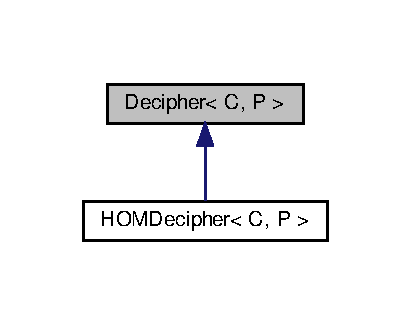
\includegraphics[width=197pt]{classDecipher__inherit__graph}
\end{center}
\end{figure}
\subsection*{Public Member Functions}
\begin{DoxyCompactItemize}
\item 
\hyperlink{classDecipher_a08c3ce832e3884da97f36fcfac6f70db}{Decipher} ()
\item 
virtual \hyperlink{classDecipher_af1489f4e86a28217bdee9cf16d983faf}{$\sim$\+Decipher} ()
\item 
virtual void \hyperlink{classDecipher_a39aea002012130201e12a8fa7d84dda5}{read\+Secrets\+From\+J\+S\+ON} (std\+::string \&string)=0
\item 
virtual P \hyperlink{classDecipher_ac6b8c369eda2d7e17fa90cb594cf41b6}{decrypt} (C \&ciphertext)=0
\end{DoxyCompactItemize}


\subsection{Detailed Description}
\subsubsection*{template$<$typename C, typename P$>$\newline
class Decipher$<$ C, P $>$}

Interface implemented by all deciphering classes in this library 
\begin{DoxyTemplParams}{Template Parameters}
{\em C} & Ciphertext type \\
\hline
{\em P} & Plaintext type \\
\hline
\end{DoxyTemplParams}


\subsection{Constructor \& Destructor Documentation}
\mbox{\Hypertarget{classDecipher_a08c3ce832e3884da97f36fcfac6f70db}\label{classDecipher_a08c3ce832e3884da97f36fcfac6f70db}} 
\index{Decipher@{Decipher}!Decipher@{Decipher}}
\index{Decipher@{Decipher}!Decipher@{Decipher}}
\subsubsection{\texorpdfstring{Decipher()}{Decipher()}}
{\footnotesize\ttfamily template$<$typename C, typename P$>$ \\
\hyperlink{classDecipher}{Decipher}$<$ C, P $>$\+::\hyperlink{classDecipher}{Decipher} (\begin{DoxyParamCaption}{ }\end{DoxyParamCaption})\hspace{0.3cm}{\ttfamily [inline]}}

\mbox{\Hypertarget{classDecipher_af1489f4e86a28217bdee9cf16d983faf}\label{classDecipher_af1489f4e86a28217bdee9cf16d983faf}} 
\index{Decipher@{Decipher}!````~Decipher@{$\sim$\+Decipher}}
\index{````~Decipher@{$\sim$\+Decipher}!Decipher@{Decipher}}
\subsubsection{\texorpdfstring{$\sim$\+Decipher()}{~Decipher()}}
{\footnotesize\ttfamily template$<$typename C, typename P$>$ \\
virtual \hyperlink{classDecipher}{Decipher}$<$ C, P $>$\+::$\sim$\hyperlink{classDecipher}{Decipher} (\begin{DoxyParamCaption}{ }\end{DoxyParamCaption})\hspace{0.3cm}{\ttfamily [inline]}, {\ttfamily [virtual]}}



\subsection{Member Function Documentation}
\mbox{\Hypertarget{classDecipher_ac6b8c369eda2d7e17fa90cb594cf41b6}\label{classDecipher_ac6b8c369eda2d7e17fa90cb594cf41b6}} 
\index{Decipher@{Decipher}!decrypt@{decrypt}}
\index{decrypt@{decrypt}!Decipher@{Decipher}}
\subsubsection{\texorpdfstring{decrypt()}{decrypt()}}
{\footnotesize\ttfamily template$<$typename C, typename P$>$ \\
virtual P \hyperlink{classDecipher}{Decipher}$<$ C, P $>$\+::decrypt (\begin{DoxyParamCaption}\item[{C \&}]{ciphertext }\end{DoxyParamCaption})\hspace{0.3cm}{\ttfamily [pure virtual]}}

Decrypts a ciphertext 
\begin{DoxyParams}{Parameters}
{\em ciphertext} & Ciphertext value \\
\hline
\end{DoxyParams}
\begin{DoxyReturn}{Returns}
Plaintext value 
\end{DoxyReturn}


Implemented in \hyperlink{classSSEDecrypter_afc1522b78aed502f8ca94163fc030ffa}{S\+S\+E\+Decrypter}, \hyperlink{classPolyACDDecrypter_a96626f2c267d9cc4b18ed25cb584d982}{Poly\+A\+C\+D\+Decrypter}, \hyperlink{classDETDecrypter_ac317ce154d64eb1fce4450c2b03a12d9}{D\+E\+T\+Decrypter}, \hyperlink{classHE1NDecrypter_a8e49ff8292a76884f328c566f4d1b646}{H\+E1\+N\+Decrypter}, \hyperlink{classGACDDecrypter_a92f6afd3d0a43dd5538cf6a83398ee33}{G\+A\+C\+D\+Decrypter}, \hyperlink{classHE2NDecrypter_aa92e4ddf62a0f2c4199722983e28b0c9}{H\+E2\+N\+Decrypter}, \hyperlink{classHE1Decrypter_a28cc03e8a37f321b8f805cc04b2e69e0}{H\+E1\+Decrypter}, and \hyperlink{classHE2Decrypter_a766f96cb2277fd3e4af59ca44a32d519}{H\+E2\+Decrypter}.

\mbox{\Hypertarget{classDecipher_a39aea002012130201e12a8fa7d84dda5}\label{classDecipher_a39aea002012130201e12a8fa7d84dda5}} 
\index{Decipher@{Decipher}!read\+Secrets\+From\+J\+S\+ON@{read\+Secrets\+From\+J\+S\+ON}}
\index{read\+Secrets\+From\+J\+S\+ON@{read\+Secrets\+From\+J\+S\+ON}!Decipher@{Decipher}}
\subsubsection{\texorpdfstring{read\+Secrets\+From\+J\+S\+O\+N()}{readSecretsFromJSON()}}
{\footnotesize\ttfamily template$<$typename C, typename P$>$ \\
virtual void \hyperlink{classDecipher}{Decipher}$<$ C, P $>$\+::read\+Secrets\+From\+J\+S\+ON (\begin{DoxyParamCaption}\item[{std\+::string \&}]{string }\end{DoxyParamCaption})\hspace{0.3cm}{\ttfamily [pure virtual]}}

Reads the cipher secrets in from a J\+S\+ON string 
\begin{DoxyParams}{Parameters}
{\em string} & J\+S\+ON string \\
\hline
\end{DoxyParams}


Implemented in \hyperlink{classSSEDecrypter_a1bdc685b8ea9c5bcc2b29f0c9a3ca7bf}{S\+S\+E\+Decrypter}, \hyperlink{classPolyACDDecrypter_a55e7f81c6d8d10e00e072547ac68239a}{Poly\+A\+C\+D\+Decrypter}, \hyperlink{classDETDecrypter_a8e32703400ead9c35a80549b011307d7}{D\+E\+T\+Decrypter}, \hyperlink{classGACDDecrypter_a7634cc069e61c1a3cf2443fed7c2b15f}{G\+A\+C\+D\+Decrypter}, \hyperlink{classHE1NDecrypter_a323f074a37cb4ebfbcfca4b6bdfb6737}{H\+E1\+N\+Decrypter}, \hyperlink{classHE2NDecrypter_a92b463d8e18d2f06d0680528edfd49c4}{H\+E2\+N\+Decrypter}, \hyperlink{classHE1Decrypter_af60ccc6d0afe7555a9d1468ad7047733}{H\+E1\+Decrypter}, and \hyperlink{classHE2Decrypter_a9cf1a6eae2667f6e891237589c4eeda0}{H\+E2\+Decrypter}.



The documentation for this class was generated from the following file\+:\begin{DoxyCompactItemize}
\item 
include/\hyperlink{Decipher_8hpp}{Decipher.\+hpp}\end{DoxyCompactItemize}

\hypertarget{classDETDecrypter}{}\section{D\+E\+T\+Decrypter Class Reference}
\label{classDETDecrypter}\index{D\+E\+T\+Decrypter@{D\+E\+T\+Decrypter}}


{\ttfamily \#include $<$D\+E\+T\+Decrypter.\+h$>$}



Inheritance diagram for D\+E\+T\+Decrypter\+:\nopagebreak
\begin{figure}[H]
\begin{center}
\leavevmode
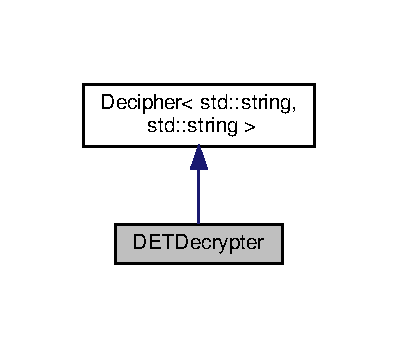
\includegraphics[width=191pt]{classDETDecrypter__inherit__graph}
\end{center}
\end{figure}


Collaboration diagram for D\+E\+T\+Decrypter\+:\nopagebreak
\begin{figure}[H]
\begin{center}
\leavevmode
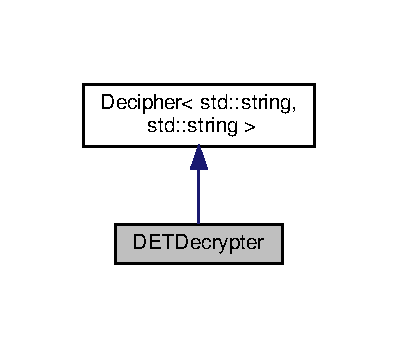
\includegraphics[width=191pt]{classDETDecrypter__coll__graph}
\end{center}
\end{figure}
\subsection*{Public Member Functions}
\begin{DoxyCompactItemize}
\item 
void \hyperlink{classDETDecrypter_a8e32703400ead9c35a80549b011307d7}{read\+Secrets\+From\+J\+S\+ON} (std\+::string \&reader) override
\item 
std\+::string \hyperlink{classDETDecrypter_ac317ce154d64eb1fce4450c2b03a12d9}{decrypt} (std\+::string \&ciphertext) override
\item 
std\+::string \hyperlink{classDETDecrypter_a1a0f8ebde80190b4d28ed071d139fc3a}{decrypt} (Crypto\+P\+P\+::\+Sec\+Byte\+Block \&ciphertext)
\item 
std\+::string \hyperlink{classDETDecrypter_acb1551670a0c4161a362f20c0eed0b3a}{decrypt\+From\+Hex} (std\+::string \&hex\+String)
\item 
void \hyperlink{classDETDecrypter_aef2cdd9235fb7d927ab4992fec6efe78}{set\+Key\+With\+IV} (Crypto\+P\+P\+::\+Sec\+Byte\+Block \&\hyperlink{classDETDecrypter_a44a998e051bc9efc04295b9401ec716e}{key}, Crypto\+P\+P\+::\+Sec\+Byte\+Block \&\hyperlink{classDETDecrypter_a601eb88318e103fd40ad1864f951ab54}{iv})
\item 
void \hyperlink{classDETDecrypter_aea297de1f5c514a5156eabc22c556b3b}{set\+Key\+With\+IV} (std\+::string \&hexkey, std\+::string \&hexiv)
\item 
\hyperlink{classDETDecrypter_af2981aa97e655d370fc77670740b16f2}{D\+E\+T\+Decrypter} ()
\item 
virtual \hyperlink{classDETDecrypter_a2d049175d238e1e657515be9048b6ab3}{$\sim$\+D\+E\+T\+Decrypter} ()
\end{DoxyCompactItemize}
\subsection*{Private Attributes}
\begin{DoxyCompactItemize}
\item 
Crypto\+P\+P\+::\+Sec\+Byte\+Block \hyperlink{classDETDecrypter_a44a998e051bc9efc04295b9401ec716e}{key}
\item 
Crypto\+P\+P\+::\+Sec\+Byte\+Block \hyperlink{classDETDecrypter_a601eb88318e103fd40ad1864f951ab54}{iv}
\item 
Crypto\+P\+P\+::\+C\+B\+C\+\_\+\+Mode$<$ Crypto\+P\+P\+::\+A\+ES $>$\+::Decryption \hyperlink{classDETDecrypter_ab598e2e972f3052d372f37d39aae07cf}{d}
\end{DoxyCompactItemize}


\subsection{Constructor \& Destructor Documentation}
\mbox{\Hypertarget{classDETDecrypter_af2981aa97e655d370fc77670740b16f2}\label{classDETDecrypter_af2981aa97e655d370fc77670740b16f2}} 
\index{D\+E\+T\+Decrypter@{D\+E\+T\+Decrypter}!D\+E\+T\+Decrypter@{D\+E\+T\+Decrypter}}
\index{D\+E\+T\+Decrypter@{D\+E\+T\+Decrypter}!D\+E\+T\+Decrypter@{D\+E\+T\+Decrypter}}
\subsubsection{\texorpdfstring{D\+E\+T\+Decrypter()}{DETDecrypter()}}
{\footnotesize\ttfamily D\+E\+T\+Decrypter\+::\+D\+E\+T\+Decrypter (\begin{DoxyParamCaption}{ }\end{DoxyParamCaption})\hspace{0.3cm}{\ttfamily [inline]}}

\mbox{\Hypertarget{classDETDecrypter_a2d049175d238e1e657515be9048b6ab3}\label{classDETDecrypter_a2d049175d238e1e657515be9048b6ab3}} 
\index{D\+E\+T\+Decrypter@{D\+E\+T\+Decrypter}!````~D\+E\+T\+Decrypter@{$\sim$\+D\+E\+T\+Decrypter}}
\index{````~D\+E\+T\+Decrypter@{$\sim$\+D\+E\+T\+Decrypter}!D\+E\+T\+Decrypter@{D\+E\+T\+Decrypter}}
\subsubsection{\texorpdfstring{$\sim$\+D\+E\+T\+Decrypter()}{~DETDecrypter()}}
{\footnotesize\ttfamily virtual D\+E\+T\+Decrypter\+::$\sim$\+D\+E\+T\+Decrypter (\begin{DoxyParamCaption}{ }\end{DoxyParamCaption})\hspace{0.3cm}{\ttfamily [inline]}, {\ttfamily [virtual]}}



\subsection{Member Function Documentation}
\mbox{\Hypertarget{classDETDecrypter_ac317ce154d64eb1fce4450c2b03a12d9}\label{classDETDecrypter_ac317ce154d64eb1fce4450c2b03a12d9}} 
\index{D\+E\+T\+Decrypter@{D\+E\+T\+Decrypter}!decrypt@{decrypt}}
\index{decrypt@{decrypt}!D\+E\+T\+Decrypter@{D\+E\+T\+Decrypter}}
\subsubsection{\texorpdfstring{decrypt()}{decrypt()}\hspace{0.1cm}{\footnotesize\ttfamily [1/2]}}
{\footnotesize\ttfamily std\+::string D\+E\+T\+Decrypter\+::decrypt (\begin{DoxyParamCaption}\item[{std\+::string \&}]{ciphertext }\end{DoxyParamCaption})\hspace{0.3cm}{\ttfamily [override]}, {\ttfamily [virtual]}}

Decrypts a ciphertext 
\begin{DoxyParams}{Parameters}
{\em ciphertext} & Ciphertext value \\
\hline
\end{DoxyParams}
\begin{DoxyReturn}{Returns}
Plaintext value 
\end{DoxyReturn}


Implements \hyperlink{classDecipher_ac6b8c369eda2d7e17fa90cb594cf41b6}{Decipher$<$ std\+::string, std\+::string $>$}.

\mbox{\Hypertarget{classDETDecrypter_a1a0f8ebde80190b4d28ed071d139fc3a}\label{classDETDecrypter_a1a0f8ebde80190b4d28ed071d139fc3a}} 
\index{D\+E\+T\+Decrypter@{D\+E\+T\+Decrypter}!decrypt@{decrypt}}
\index{decrypt@{decrypt}!D\+E\+T\+Decrypter@{D\+E\+T\+Decrypter}}
\subsubsection{\texorpdfstring{decrypt()}{decrypt()}\hspace{0.1cm}{\footnotesize\ttfamily [2/2]}}
{\footnotesize\ttfamily std\+::string D\+E\+T\+Decrypter\+::decrypt (\begin{DoxyParamCaption}\item[{Crypto\+P\+P\+::\+Sec\+Byte\+Block \&}]{ciphertext }\end{DoxyParamCaption})}

Convenience method to decrypt a byte array 
\begin{DoxyParams}{Parameters}
{\em ciphertext} & byte array \\
\hline
\end{DoxyParams}
\begin{DoxyReturn}{Returns}
plaintext byte string 
\end{DoxyReturn}
\mbox{\Hypertarget{classDETDecrypter_acb1551670a0c4161a362f20c0eed0b3a}\label{classDETDecrypter_acb1551670a0c4161a362f20c0eed0b3a}} 
\index{D\+E\+T\+Decrypter@{D\+E\+T\+Decrypter}!decrypt\+From\+Hex@{decrypt\+From\+Hex}}
\index{decrypt\+From\+Hex@{decrypt\+From\+Hex}!D\+E\+T\+Decrypter@{D\+E\+T\+Decrypter}}
\subsubsection{\texorpdfstring{decrypt\+From\+Hex()}{decryptFromHex()}}
{\footnotesize\ttfamily std\+::string D\+E\+T\+Decrypter\+::decrypt\+From\+Hex (\begin{DoxyParamCaption}\item[{std\+::string \&}]{hex\+String }\end{DoxyParamCaption})}

Convenience method to decrypt a hexadecimal encoded string 
\begin{DoxyParams}{Parameters}
{\em hex\+String} & Hexadecimal encoded string \\
\hline
\end{DoxyParams}
\begin{DoxyReturn}{Returns}
plaintext byte string 
\end{DoxyReturn}
\mbox{\Hypertarget{classDETDecrypter_a8e32703400ead9c35a80549b011307d7}\label{classDETDecrypter_a8e32703400ead9c35a80549b011307d7}} 
\index{D\+E\+T\+Decrypter@{D\+E\+T\+Decrypter}!read\+Secrets\+From\+J\+S\+ON@{read\+Secrets\+From\+J\+S\+ON}}
\index{read\+Secrets\+From\+J\+S\+ON@{read\+Secrets\+From\+J\+S\+ON}!D\+E\+T\+Decrypter@{D\+E\+T\+Decrypter}}
\subsubsection{\texorpdfstring{read\+Secrets\+From\+J\+S\+O\+N()}{readSecretsFromJSON()}}
{\footnotesize\ttfamily void D\+E\+T\+Decrypter\+::read\+Secrets\+From\+J\+S\+ON (\begin{DoxyParamCaption}\item[{std\+::string \&}]{string }\end{DoxyParamCaption})\hspace{0.3cm}{\ttfamily [override]}, {\ttfamily [virtual]}}

Reads the cipher secrets in from a J\+S\+ON string 
\begin{DoxyParams}{Parameters}
{\em string} & J\+S\+ON string \\
\hline
\end{DoxyParams}


Implements \hyperlink{classDecipher_a39aea002012130201e12a8fa7d84dda5}{Decipher$<$ std\+::string, std\+::string $>$}.

\mbox{\Hypertarget{classDETDecrypter_aef2cdd9235fb7d927ab4992fec6efe78}\label{classDETDecrypter_aef2cdd9235fb7d927ab4992fec6efe78}} 
\index{D\+E\+T\+Decrypter@{D\+E\+T\+Decrypter}!set\+Key\+With\+IV@{set\+Key\+With\+IV}}
\index{set\+Key\+With\+IV@{set\+Key\+With\+IV}!D\+E\+T\+Decrypter@{D\+E\+T\+Decrypter}}
\subsubsection{\texorpdfstring{set\+Key\+With\+I\+V()}{setKeyWithIV()}\hspace{0.1cm}{\footnotesize\ttfamily [1/2]}}
{\footnotesize\ttfamily void D\+E\+T\+Decrypter\+::set\+Key\+With\+IV (\begin{DoxyParamCaption}\item[{Crypto\+P\+P\+::\+Sec\+Byte\+Block \&}]{key,  }\item[{Crypto\+P\+P\+::\+Sec\+Byte\+Block \&}]{iv }\end{DoxyParamCaption})}

Accessor to set the A\+ES cipher key and initialisation vector 
\begin{DoxyParams}{Parameters}
{\em key} & A\+ES key (byte array) \\
\hline
{\em iv} & A\+ES initiialisation vector (byte array) \\
\hline
\end{DoxyParams}
\mbox{\Hypertarget{classDETDecrypter_aea297de1f5c514a5156eabc22c556b3b}\label{classDETDecrypter_aea297de1f5c514a5156eabc22c556b3b}} 
\index{D\+E\+T\+Decrypter@{D\+E\+T\+Decrypter}!set\+Key\+With\+IV@{set\+Key\+With\+IV}}
\index{set\+Key\+With\+IV@{set\+Key\+With\+IV}!D\+E\+T\+Decrypter@{D\+E\+T\+Decrypter}}
\subsubsection{\texorpdfstring{set\+Key\+With\+I\+V()}{setKeyWithIV()}\hspace{0.1cm}{\footnotesize\ttfamily [2/2]}}
{\footnotesize\ttfamily void D\+E\+T\+Decrypter\+::set\+Key\+With\+IV (\begin{DoxyParamCaption}\item[{std\+::string \&}]{hexkey,  }\item[{std\+::string \&}]{hexiv }\end{DoxyParamCaption})}

Accessor to set the A\+ES cipher key and initialisation vector 
\begin{DoxyParams}{Parameters}
{\em hexkey} & Hexadecimal encoded A\+ES key \\
\hline
{\em hexiv} & Hexadecimal encoded initialisation vector \\
\hline
\end{DoxyParams}


\subsection{Member Data Documentation}
\mbox{\Hypertarget{classDETDecrypter_ab598e2e972f3052d372f37d39aae07cf}\label{classDETDecrypter_ab598e2e972f3052d372f37d39aae07cf}} 
\index{D\+E\+T\+Decrypter@{D\+E\+T\+Decrypter}!d@{d}}
\index{d@{d}!D\+E\+T\+Decrypter@{D\+E\+T\+Decrypter}}
\subsubsection{\texorpdfstring{d}{d}}
{\footnotesize\ttfamily Crypto\+P\+P\+::\+C\+B\+C\+\_\+\+Mode$<$Crypto\+P\+P\+::\+A\+ES$>$\+::Decryption D\+E\+T\+Decrypter\+::d\hspace{0.3cm}{\ttfamily [private]}}

C\+BC mode A\+ES decryption. \mbox{\Hypertarget{classDETDecrypter_a601eb88318e103fd40ad1864f951ab54}\label{classDETDecrypter_a601eb88318e103fd40ad1864f951ab54}} 
\index{D\+E\+T\+Decrypter@{D\+E\+T\+Decrypter}!iv@{iv}}
\index{iv@{iv}!D\+E\+T\+Decrypter@{D\+E\+T\+Decrypter}}
\subsubsection{\texorpdfstring{iv}{iv}}
{\footnotesize\ttfamily Crypto\+P\+P\+::\+Sec\+Byte\+Block D\+E\+T\+Decrypter\+::iv\hspace{0.3cm}{\ttfamily [private]}}

A\+ES initialisation vector (byte array) \mbox{\Hypertarget{classDETDecrypter_a44a998e051bc9efc04295b9401ec716e}\label{classDETDecrypter_a44a998e051bc9efc04295b9401ec716e}} 
\index{D\+E\+T\+Decrypter@{D\+E\+T\+Decrypter}!key@{key}}
\index{key@{key}!D\+E\+T\+Decrypter@{D\+E\+T\+Decrypter}}
\subsubsection{\texorpdfstring{key}{key}}
{\footnotesize\ttfamily Crypto\+P\+P\+::\+Sec\+Byte\+Block D\+E\+T\+Decrypter\+::key\hspace{0.3cm}{\ttfamily [private]}}

A\+ES key (byte array) 

The documentation for this class was generated from the following files\+:\begin{DoxyCompactItemize}
\item 
include/\hyperlink{DETDecrypter_8h}{D\+E\+T\+Decrypter.\+h}\item 
src/\hyperlink{DETDecrypter_8cpp}{D\+E\+T\+Decrypter.\+cpp}\end{DoxyCompactItemize}

\hypertarget{classDETEncrypter}{}\section{D\+E\+T\+Encrypter Class Reference}
\label{classDETEncrypter}\index{D\+E\+T\+Encrypter@{D\+E\+T\+Encrypter}}


{\ttfamily \#include $<$D\+E\+T\+Encrypter.\+h$>$}



Inheritance diagram for D\+E\+T\+Encrypter\+:\nopagebreak
\begin{figure}[H]
\begin{center}
\leavevmode
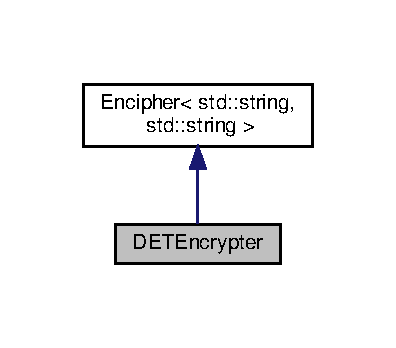
\includegraphics[width=190pt]{classDETEncrypter__inherit__graph}
\end{center}
\end{figure}


Collaboration diagram for D\+E\+T\+Encrypter\+:\nopagebreak
\begin{figure}[H]
\begin{center}
\leavevmode
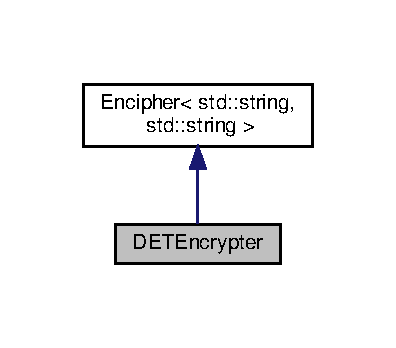
\includegraphics[width=190pt]{classDETEncrypter__coll__graph}
\end{center}
\end{figure}
\subsection*{Public Member Functions}
\begin{DoxyCompactItemize}
\item 
std\+::string \hyperlink{classDETEncrypter_a9d628bff7fe333ece3c39f3827727582}{encrypt} (std\+::string \&plaintext) override
\item 
std\+::string \hyperlink{classDETEncrypter_a0755264964442bb1593cf1ffd0bbe274}{encrypt} (Crypto\+P\+P\+::\+Sec\+Byte\+Block \&plaintext)
\item 
std\+::string \hyperlink{classDETEncrypter_ad688722b05535c623af3c32548af23c9}{encrypt\+To\+Hex} (std\+::string \&plaintext)
\item 
std\+::string \hyperlink{classDETEncrypter_a78128a4a9df72a4199abbd06f6169c48}{encrypt\+To\+Hex} (Crypto\+P\+P\+::\+Sec\+Byte\+Block \&plaintext)
\item 
Crypto\+P\+P\+::\+Sec\+Byte\+Block \hyperlink{classDETEncrypter_aa8b1e2a9a97067e338eaf5f4b6093db9}{get\+Key} ()
\item 
Crypto\+P\+P\+::\+Sec\+Byte\+Block \hyperlink{classDETEncrypter_a78968a6f219de6c9d08989898d954e30}{get\+IV} ()
\item 
std\+::string \hyperlink{classDETEncrypter_a79402704553f39cc751cc60c5ace53df}{get\+Hex\+Encoded\+Key} ()
\item 
std\+::string \hyperlink{classDETEncrypter_adebcf0d8c18e5b994a8f6cc3e29edff6}{get\+Hex\+Encoded\+IV} ()
\item 
std\+::string \hyperlink{classDETEncrypter_a30ffe8f94a95f723e62d0b1a1ed8dc56}{write\+Secrets\+To\+J\+S\+ON} () override
\item 
\hyperlink{classDETEncrypter_a11abdce8bc5cda79b1d3f20b940a99d1}{D\+E\+T\+Encrypter} ()
\item 
virtual \hyperlink{classDETEncrypter_a517bdbe6dfd178ebb66405faa9cfca55}{$\sim$\+D\+E\+T\+Encrypter} ()
\end{DoxyCompactItemize}
\subsection*{Private Attributes}
\begin{DoxyCompactItemize}
\item 
Crypto\+P\+P\+::\+Sec\+Byte\+Block \hyperlink{classDETEncrypter_a698a78e4f1fb49cf02a005ee7bce6a99}{key}
\item 
Crypto\+P\+P\+::\+Sec\+Byte\+Block \hyperlink{classDETEncrypter_a40e99abf751fa9c802b3a4cc9c6796a0}{iv}
\item 
Crypto\+P\+P\+::\+C\+B\+C\+\_\+\+Mode$<$ Crypto\+P\+P\+::\+A\+ES $>$\+::Encryption \hyperlink{classDETEncrypter_a29875af9a8c1df01802d11f0a00f5f90}{e}
\end{DoxyCompactItemize}


\subsection{Constructor \& Destructor Documentation}
\mbox{\Hypertarget{classDETEncrypter_a11abdce8bc5cda79b1d3f20b940a99d1}\label{classDETEncrypter_a11abdce8bc5cda79b1d3f20b940a99d1}} 
\index{D\+E\+T\+Encrypter@{D\+E\+T\+Encrypter}!D\+E\+T\+Encrypter@{D\+E\+T\+Encrypter}}
\index{D\+E\+T\+Encrypter@{D\+E\+T\+Encrypter}!D\+E\+T\+Encrypter@{D\+E\+T\+Encrypter}}
\subsubsection{\texorpdfstring{D\+E\+T\+Encrypter()}{DETEncrypter()}}
{\footnotesize\ttfamily D\+E\+T\+Encrypter\+::\+D\+E\+T\+Encrypter (\begin{DoxyParamCaption}{ }\end{DoxyParamCaption})}

The constructor generates a random 256-\/bit key and initialisation vector. \mbox{\Hypertarget{classDETEncrypter_a517bdbe6dfd178ebb66405faa9cfca55}\label{classDETEncrypter_a517bdbe6dfd178ebb66405faa9cfca55}} 
\index{D\+E\+T\+Encrypter@{D\+E\+T\+Encrypter}!````~D\+E\+T\+Encrypter@{$\sim$\+D\+E\+T\+Encrypter}}
\index{````~D\+E\+T\+Encrypter@{$\sim$\+D\+E\+T\+Encrypter}!D\+E\+T\+Encrypter@{D\+E\+T\+Encrypter}}
\subsubsection{\texorpdfstring{$\sim$\+D\+E\+T\+Encrypter()}{~DETEncrypter()}}
{\footnotesize\ttfamily virtual D\+E\+T\+Encrypter\+::$\sim$\+D\+E\+T\+Encrypter (\begin{DoxyParamCaption}{ }\end{DoxyParamCaption})\hspace{0.3cm}{\ttfamily [inline]}, {\ttfamily [virtual]}}



\subsection{Member Function Documentation}
\mbox{\Hypertarget{classDETEncrypter_a9d628bff7fe333ece3c39f3827727582}\label{classDETEncrypter_a9d628bff7fe333ece3c39f3827727582}} 
\index{D\+E\+T\+Encrypter@{D\+E\+T\+Encrypter}!encrypt@{encrypt}}
\index{encrypt@{encrypt}!D\+E\+T\+Encrypter@{D\+E\+T\+Encrypter}}
\subsubsection{\texorpdfstring{encrypt()}{encrypt()}\hspace{0.1cm}{\footnotesize\ttfamily [1/2]}}
{\footnotesize\ttfamily std\+::string D\+E\+T\+Encrypter\+::encrypt (\begin{DoxyParamCaption}\item[{std\+::string \&}]{plaintext }\end{DoxyParamCaption})\hspace{0.3cm}{\ttfamily [override]}, {\ttfamily [virtual]}}

Encrypt a plaintext 
\begin{DoxyParams}{Parameters}
{\em plaintext} & A plaintext value \\
\hline
\end{DoxyParams}
\begin{DoxyReturn}{Returns}
A ciphertext value 
\end{DoxyReturn}


Implements \hyperlink{classEncipher_aaf8138eb280608bfd03c6eb762ffc010}{Encipher$<$ std\+::string, std\+::string $>$}.

\mbox{\Hypertarget{classDETEncrypter_a0755264964442bb1593cf1ffd0bbe274}\label{classDETEncrypter_a0755264964442bb1593cf1ffd0bbe274}} 
\index{D\+E\+T\+Encrypter@{D\+E\+T\+Encrypter}!encrypt@{encrypt}}
\index{encrypt@{encrypt}!D\+E\+T\+Encrypter@{D\+E\+T\+Encrypter}}
\subsubsection{\texorpdfstring{encrypt()}{encrypt()}\hspace{0.1cm}{\footnotesize\ttfamily [2/2]}}
{\footnotesize\ttfamily std\+::string D\+E\+T\+Encrypter\+::encrypt (\begin{DoxyParamCaption}\item[{Crypto\+P\+P\+::\+Sec\+Byte\+Block \&}]{plaintext }\end{DoxyParamCaption})}

A convenience method to encrypt a byte array 
\begin{DoxyParams}{Parameters}
{\em plaintext} & A byte array \\
\hline
\end{DoxyParams}
\begin{DoxyReturn}{Returns}
A ciphertext as a byte string 
\end{DoxyReturn}
\mbox{\Hypertarget{classDETEncrypter_ad688722b05535c623af3c32548af23c9}\label{classDETEncrypter_ad688722b05535c623af3c32548af23c9}} 
\index{D\+E\+T\+Encrypter@{D\+E\+T\+Encrypter}!encrypt\+To\+Hex@{encrypt\+To\+Hex}}
\index{encrypt\+To\+Hex@{encrypt\+To\+Hex}!D\+E\+T\+Encrypter@{D\+E\+T\+Encrypter}}
\subsubsection{\texorpdfstring{encrypt\+To\+Hex()}{encryptToHex()}\hspace{0.1cm}{\footnotesize\ttfamily [1/2]}}
{\footnotesize\ttfamily std\+::string D\+E\+T\+Encrypter\+::encrypt\+To\+Hex (\begin{DoxyParamCaption}\item[{std\+::string \&}]{plaintext }\end{DoxyParamCaption})}

A convenience method to encrypt to a hexadecimal encoded string 
\begin{DoxyParams}{Parameters}
{\em plaintext} & A (byte) string \\
\hline
\end{DoxyParams}
\begin{DoxyReturn}{Returns}
A hexadecimal encoded string 
\end{DoxyReturn}
\mbox{\Hypertarget{classDETEncrypter_a78128a4a9df72a4199abbd06f6169c48}\label{classDETEncrypter_a78128a4a9df72a4199abbd06f6169c48}} 
\index{D\+E\+T\+Encrypter@{D\+E\+T\+Encrypter}!encrypt\+To\+Hex@{encrypt\+To\+Hex}}
\index{encrypt\+To\+Hex@{encrypt\+To\+Hex}!D\+E\+T\+Encrypter@{D\+E\+T\+Encrypter}}
\subsubsection{\texorpdfstring{encrypt\+To\+Hex()}{encryptToHex()}\hspace{0.1cm}{\footnotesize\ttfamily [2/2]}}
{\footnotesize\ttfamily std\+::string D\+E\+T\+Encrypter\+::encrypt\+To\+Hex (\begin{DoxyParamCaption}\item[{Crypto\+P\+P\+::\+Sec\+Byte\+Block \&}]{plaintext }\end{DoxyParamCaption})}

A convenience method to encrypt a byte array to a hexadecimal encoded string 
\begin{DoxyParams}{Parameters}
{\em plaintext} & A byte array \\
\hline
\end{DoxyParams}
\begin{DoxyReturn}{Returns}
A hexadecimal encoded string 
\end{DoxyReturn}
\mbox{\Hypertarget{classDETEncrypter_adebcf0d8c18e5b994a8f6cc3e29edff6}\label{classDETEncrypter_adebcf0d8c18e5b994a8f6cc3e29edff6}} 
\index{D\+E\+T\+Encrypter@{D\+E\+T\+Encrypter}!get\+Hex\+Encoded\+IV@{get\+Hex\+Encoded\+IV}}
\index{get\+Hex\+Encoded\+IV@{get\+Hex\+Encoded\+IV}!D\+E\+T\+Encrypter@{D\+E\+T\+Encrypter}}
\subsubsection{\texorpdfstring{get\+Hex\+Encoded\+I\+V()}{getHexEncodedIV()}}
{\footnotesize\ttfamily std\+::string D\+E\+T\+Encrypter\+::get\+Hex\+Encoded\+IV (\begin{DoxyParamCaption}{ }\end{DoxyParamCaption})}

Convenience method to get the initialisation vector as a hexadecimal encoded string \begin{DoxyReturn}{Returns}
A hexadecimal encoded string 
\end{DoxyReturn}
\mbox{\Hypertarget{classDETEncrypter_a79402704553f39cc751cc60c5ace53df}\label{classDETEncrypter_a79402704553f39cc751cc60c5ace53df}} 
\index{D\+E\+T\+Encrypter@{D\+E\+T\+Encrypter}!get\+Hex\+Encoded\+Key@{get\+Hex\+Encoded\+Key}}
\index{get\+Hex\+Encoded\+Key@{get\+Hex\+Encoded\+Key}!D\+E\+T\+Encrypter@{D\+E\+T\+Encrypter}}
\subsubsection{\texorpdfstring{get\+Hex\+Encoded\+Key()}{getHexEncodedKey()}}
{\footnotesize\ttfamily std\+::string D\+E\+T\+Encrypter\+::get\+Hex\+Encoded\+Key (\begin{DoxyParamCaption}{ }\end{DoxyParamCaption})}

Convenience method to get the key as a hexadecimal encoded string \begin{DoxyReturn}{Returns}
A hexadecimal encoded string 
\end{DoxyReturn}
\mbox{\Hypertarget{classDETEncrypter_a78968a6f219de6c9d08989898d954e30}\label{classDETEncrypter_a78968a6f219de6c9d08989898d954e30}} 
\index{D\+E\+T\+Encrypter@{D\+E\+T\+Encrypter}!get\+IV@{get\+IV}}
\index{get\+IV@{get\+IV}!D\+E\+T\+Encrypter@{D\+E\+T\+Encrypter}}
\subsubsection{\texorpdfstring{get\+I\+V()}{getIV()}}
{\footnotesize\ttfamily Crypto\+P\+P\+::\+Sec\+Byte\+Block D\+E\+T\+Encrypter\+::get\+IV (\begin{DoxyParamCaption}{ }\end{DoxyParamCaption})}

Returns the C\+BC mode initialisation vector as a byte array \begin{DoxyReturn}{Returns}
Byte array 
\end{DoxyReturn}
\mbox{\Hypertarget{classDETEncrypter_aa8b1e2a9a97067e338eaf5f4b6093db9}\label{classDETEncrypter_aa8b1e2a9a97067e338eaf5f4b6093db9}} 
\index{D\+E\+T\+Encrypter@{D\+E\+T\+Encrypter}!get\+Key@{get\+Key}}
\index{get\+Key@{get\+Key}!D\+E\+T\+Encrypter@{D\+E\+T\+Encrypter}}
\subsubsection{\texorpdfstring{get\+Key()}{getKey()}}
{\footnotesize\ttfamily Crypto\+P\+P\+::\+Sec\+Byte\+Block D\+E\+T\+Encrypter\+::get\+Key (\begin{DoxyParamCaption}{ }\end{DoxyParamCaption})}

Return the key material as a byte aray \begin{DoxyReturn}{Returns}
Byte array 
\end{DoxyReturn}
\mbox{\Hypertarget{classDETEncrypter_a30ffe8f94a95f723e62d0b1a1ed8dc56}\label{classDETEncrypter_a30ffe8f94a95f723e62d0b1a1ed8dc56}} 
\index{D\+E\+T\+Encrypter@{D\+E\+T\+Encrypter}!write\+Secrets\+To\+J\+S\+ON@{write\+Secrets\+To\+J\+S\+ON}}
\index{write\+Secrets\+To\+J\+S\+ON@{write\+Secrets\+To\+J\+S\+ON}!D\+E\+T\+Encrypter@{D\+E\+T\+Encrypter}}
\subsubsection{\texorpdfstring{write\+Secrets\+To\+J\+S\+O\+N()}{writeSecretsToJSON()}}
{\footnotesize\ttfamily std\+::string D\+E\+T\+Encrypter\+::write\+Secrets\+To\+J\+S\+ON (\begin{DoxyParamCaption}{ }\end{DoxyParamCaption})\hspace{0.3cm}{\ttfamily [override]}, {\ttfamily [virtual]}}

Writes cipher secrets out to a J\+S\+ON string \begin{DoxyReturn}{Returns}
J\+S\+ON string 
\end{DoxyReturn}


Implements \hyperlink{classEncipher_a27d3efa1e364c1f0d7def65454c61b85}{Encipher$<$ std\+::string, std\+::string $>$}.



\subsection{Member Data Documentation}
\mbox{\Hypertarget{classDETEncrypter_a29875af9a8c1df01802d11f0a00f5f90}\label{classDETEncrypter_a29875af9a8c1df01802d11f0a00f5f90}} 
\index{D\+E\+T\+Encrypter@{D\+E\+T\+Encrypter}!e@{e}}
\index{e@{e}!D\+E\+T\+Encrypter@{D\+E\+T\+Encrypter}}
\subsubsection{\texorpdfstring{e}{e}}
{\footnotesize\ttfamily Crypto\+P\+P\+::\+C\+B\+C\+\_\+\+Mode$<$Crypto\+P\+P\+::\+A\+ES$>$\+::Encryption D\+E\+T\+Encrypter\+::e\hspace{0.3cm}{\ttfamily [private]}}

C\+BC mode A\+ES encryption \mbox{\Hypertarget{classDETEncrypter_a40e99abf751fa9c802b3a4cc9c6796a0}\label{classDETEncrypter_a40e99abf751fa9c802b3a4cc9c6796a0}} 
\index{D\+E\+T\+Encrypter@{D\+E\+T\+Encrypter}!iv@{iv}}
\index{iv@{iv}!D\+E\+T\+Encrypter@{D\+E\+T\+Encrypter}}
\subsubsection{\texorpdfstring{iv}{iv}}
{\footnotesize\ttfamily Crypto\+P\+P\+::\+Sec\+Byte\+Block D\+E\+T\+Encrypter\+::iv\hspace{0.3cm}{\ttfamily [private]}}

A\+ES C\+BC (Cipher Block Chaining) mode initialization vector (byte array) \mbox{\Hypertarget{classDETEncrypter_a698a78e4f1fb49cf02a005ee7bce6a99}\label{classDETEncrypter_a698a78e4f1fb49cf02a005ee7bce6a99}} 
\index{D\+E\+T\+Encrypter@{D\+E\+T\+Encrypter}!key@{key}}
\index{key@{key}!D\+E\+T\+Encrypter@{D\+E\+T\+Encrypter}}
\subsubsection{\texorpdfstring{key}{key}}
{\footnotesize\ttfamily Crypto\+P\+P\+::\+Sec\+Byte\+Block D\+E\+T\+Encrypter\+::key\hspace{0.3cm}{\ttfamily [private]}}

The A\+ES cipher key (byte array) 

The documentation for this class was generated from the following files\+:\begin{DoxyCompactItemize}
\item 
include/\hyperlink{DETEncrypter_8h}{D\+E\+T\+Encrypter.\+h}\item 
src/\hyperlink{DETEncrypter_8cpp}{D\+E\+T\+Encrypter.\+cpp}\end{DoxyCompactItemize}

\hypertarget{classEncipher}{}\section{Encipher$<$ C, P $>$ Class Template Reference}
\label{classEncipher}\index{Encipher$<$ C, P $>$@{Encipher$<$ C, P $>$}}


{\ttfamily \#include $<$Encipher.\+hpp$>$}



Inheritance diagram for Encipher$<$ C, P $>$\+:
\nopagebreak
\begin{figure}[H]
\begin{center}
\leavevmode
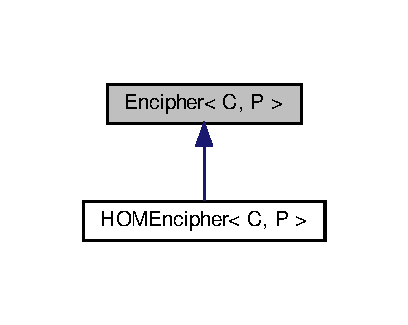
\includegraphics[width=196pt]{classEncipher__inherit__graph}
\end{center}
\end{figure}
\subsection*{Public Member Functions}
\begin{DoxyCompactItemize}
\item 
\hyperlink{classEncipher_a0d082b8ecd382929d4592e094c0028a6}{Encipher} ()
\item 
virtual \hyperlink{classEncipher_a0960dbd85f3b203438e16d2027e557fa}{$\sim$\+Encipher} ()
\item 
virtual std\+::string \hyperlink{classEncipher_a27d3efa1e364c1f0d7def65454c61b85}{write\+Secrets\+To\+J\+S\+ON} ()=0
\item 
virtual C \hyperlink{classEncipher_aaf8138eb280608bfd03c6eb762ffc010}{encrypt} (P \&plaintext)=0
\end{DoxyCompactItemize}


\subsection{Constructor \& Destructor Documentation}
\mbox{\Hypertarget{classEncipher_a0d082b8ecd382929d4592e094c0028a6}\label{classEncipher_a0d082b8ecd382929d4592e094c0028a6}} 
\index{Encipher@{Encipher}!Encipher@{Encipher}}
\index{Encipher@{Encipher}!Encipher@{Encipher}}
\subsubsection{\texorpdfstring{Encipher()}{Encipher()}}
{\footnotesize\ttfamily template$<$typename C, typename P$>$ \\
\hyperlink{classEncipher}{Encipher}$<$ C, P $>$\+::\hyperlink{classEncipher}{Encipher} (\begin{DoxyParamCaption}{ }\end{DoxyParamCaption})\hspace{0.3cm}{\ttfamily [inline]}}

\mbox{\Hypertarget{classEncipher_a0960dbd85f3b203438e16d2027e557fa}\label{classEncipher_a0960dbd85f3b203438e16d2027e557fa}} 
\index{Encipher@{Encipher}!````~Encipher@{$\sim$\+Encipher}}
\index{````~Encipher@{$\sim$\+Encipher}!Encipher@{Encipher}}
\subsubsection{\texorpdfstring{$\sim$\+Encipher()}{~Encipher()}}
{\footnotesize\ttfamily template$<$typename C, typename P$>$ \\
virtual \hyperlink{classEncipher}{Encipher}$<$ C, P $>$\+::$\sim$\hyperlink{classEncipher}{Encipher} (\begin{DoxyParamCaption}{ }\end{DoxyParamCaption})\hspace{0.3cm}{\ttfamily [inline]}, {\ttfamily [virtual]}}



\subsection{Member Function Documentation}
\mbox{\Hypertarget{classEncipher_aaf8138eb280608bfd03c6eb762ffc010}\label{classEncipher_aaf8138eb280608bfd03c6eb762ffc010}} 
\index{Encipher@{Encipher}!encrypt@{encrypt}}
\index{encrypt@{encrypt}!Encipher@{Encipher}}
\subsubsection{\texorpdfstring{encrypt()}{encrypt()}}
{\footnotesize\ttfamily template$<$typename C, typename P$>$ \\
virtual C \hyperlink{classEncipher}{Encipher}$<$ C, P $>$\+::encrypt (\begin{DoxyParamCaption}\item[{P \&}]{plaintext }\end{DoxyParamCaption})\hspace{0.3cm}{\ttfamily [pure virtual]}}



Implemented in \hyperlink{classSSEEncrypter_ab13571d2a7a8875226bf8901cd080949}{S\+S\+E\+Encrypter}, \hyperlink{classPolyACDEncrypter_a5233a73398d39d93567392c64a120e1e}{Poly\+A\+C\+D\+Encrypter}, \hyperlink{classGACDEncrypter_a310a857f6b77a6c83d4319968d49902f}{G\+A\+C\+D\+Encrypter}, \hyperlink{classDETEncrypter_a9d628bff7fe333ece3c39f3827727582}{D\+E\+T\+Encrypter}, \hyperlink{classHE1NEncrypter_a9a9c76558466ac56093cb6da937c7fe3}{H\+E1\+N\+Encrypter}, \hyperlink{classHE2NEncrypter_aa7ae559f2407b7a5527bd42470224e1b}{H\+E2\+N\+Encrypter}, \hyperlink{classHE2Encrypter_a57e4bdacbab9b11467f26deab921d134}{H\+E2\+Encrypter}, and \hyperlink{classHE1Encrypter_afc178d8e27a1263bef824bfc8960dbc0}{H\+E1\+Encrypter}.

\mbox{\Hypertarget{classEncipher_a27d3efa1e364c1f0d7def65454c61b85}\label{classEncipher_a27d3efa1e364c1f0d7def65454c61b85}} 
\index{Encipher@{Encipher}!write\+Secrets\+To\+J\+S\+ON@{write\+Secrets\+To\+J\+S\+ON}}
\index{write\+Secrets\+To\+J\+S\+ON@{write\+Secrets\+To\+J\+S\+ON}!Encipher@{Encipher}}
\subsubsection{\texorpdfstring{write\+Secrets\+To\+J\+S\+O\+N()}{writeSecretsToJSON()}}
{\footnotesize\ttfamily template$<$typename C, typename P$>$ \\
virtual std\+::string \hyperlink{classEncipher}{Encipher}$<$ C, P $>$\+::write\+Secrets\+To\+J\+S\+ON (\begin{DoxyParamCaption}{ }\end{DoxyParamCaption})\hspace{0.3cm}{\ttfamily [pure virtual]}}



Implemented in \hyperlink{classSSEEncrypter_a70e01b58fe0de0931cdb00ee97ee4af9}{S\+S\+E\+Encrypter}, \hyperlink{classDETEncrypter_a30ffe8f94a95f723e62d0b1a1ed8dc56}{D\+E\+T\+Encrypter}, \hyperlink{classPolyACDEncrypter_af478f2fe3f886d23749955eaa72e413b}{Poly\+A\+C\+D\+Encrypter}, \hyperlink{classGACDEncrypter_a01cd18ae81d0d28076c4ceb690a8b418}{G\+A\+C\+D\+Encrypter}, \hyperlink{classHE1NEncrypter_ad1bca3e0933b8e15b91d208e421f83b2}{H\+E1\+N\+Encrypter}, \hyperlink{classHE2NEncrypter_a720d4ee52dadd55f61631554d2942a6b}{H\+E2\+N\+Encrypter}, \hyperlink{classHE1Encrypter_a05627c66faf89c133a24fa7bb4553ef2}{H\+E1\+Encrypter}, and \hyperlink{classHE2Encrypter_a8cdf863bfbe046b4e57322adf5addddb}{H\+E2\+Encrypter}.



The documentation for this class was generated from the following file\+:\begin{DoxyCompactItemize}
\item 
include/\hyperlink{Encipher_8hpp}{Encipher.\+hpp}\end{DoxyCompactItemize}

\hypertarget{classGACDDecrypter}{}\section{G\+A\+C\+D\+Decrypter Class Reference}
\label{classGACDDecrypter}\index{G\+A\+C\+D\+Decrypter@{G\+A\+C\+D\+Decrypter}}


{\ttfamily \#include $<$G\+A\+C\+D\+Decrypter.\+h$>$}



Inheritance diagram for G\+A\+C\+D\+Decrypter\+:\nopagebreak
\begin{figure}[H]
\begin{center}
\leavevmode
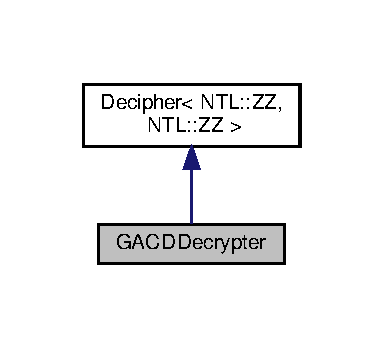
\includegraphics[width=184pt]{classGACDDecrypter__inherit__graph}
\end{center}
\end{figure}


Collaboration diagram for G\+A\+C\+D\+Decrypter\+:\nopagebreak
\begin{figure}[H]
\begin{center}
\leavevmode
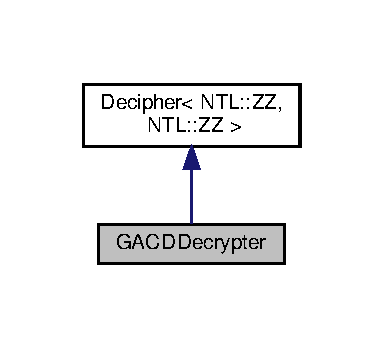
\includegraphics[width=184pt]{classGACDDecrypter__coll__graph}
\end{center}
\end{figure}
\subsection*{Public Member Functions}
\begin{DoxyCompactItemize}
\item 
\hyperlink{classGACDDecrypter_a3ce2ad60f6e2a6bb5e474df80e65a61d}{G\+A\+C\+D\+Decrypter} ()
\item 
virtual \hyperlink{classGACDDecrypter_a9f940e67f5747fe8052de483531ebfbf}{$\sim$\+G\+A\+C\+D\+Decrypter} ()
\item 
N\+T\+L\+::\+ZZ \hyperlink{classGACDDecrypter_a92f6afd3d0a43dd5538cf6a83398ee33}{decrypt} (N\+T\+L\+::\+ZZ \&ciphertext) override
\item 
void \hyperlink{classGACDDecrypter_a7634cc069e61c1a3cf2443fed7c2b15f}{read\+Secrets\+From\+J\+S\+ON} (std\+::string \&secrets) override
\end{DoxyCompactItemize}
\subsection*{Private Attributes}
\begin{DoxyCompactItemize}
\item 
N\+T\+L\+::\+ZZ \hyperlink{classGACDDecrypter_add375694b9dd663ac42f6244f4d8ea53}{k}
\end{DoxyCompactItemize}


\subsection{Constructor \& Destructor Documentation}
\mbox{\Hypertarget{classGACDDecrypter_a3ce2ad60f6e2a6bb5e474df80e65a61d}\label{classGACDDecrypter_a3ce2ad60f6e2a6bb5e474df80e65a61d}} 
\index{G\+A\+C\+D\+Decrypter@{G\+A\+C\+D\+Decrypter}!G\+A\+C\+D\+Decrypter@{G\+A\+C\+D\+Decrypter}}
\index{G\+A\+C\+D\+Decrypter@{G\+A\+C\+D\+Decrypter}!G\+A\+C\+D\+Decrypter@{G\+A\+C\+D\+Decrypter}}
\subsubsection{\texorpdfstring{G\+A\+C\+D\+Decrypter()}{GACDDecrypter()}}
{\footnotesize\ttfamily G\+A\+C\+D\+Decrypter\+::\+G\+A\+C\+D\+Decrypter (\begin{DoxyParamCaption}{ }\end{DoxyParamCaption})\hspace{0.3cm}{\ttfamily [inline]}}

\mbox{\Hypertarget{classGACDDecrypter_a9f940e67f5747fe8052de483531ebfbf}\label{classGACDDecrypter_a9f940e67f5747fe8052de483531ebfbf}} 
\index{G\+A\+C\+D\+Decrypter@{G\+A\+C\+D\+Decrypter}!````~G\+A\+C\+D\+Decrypter@{$\sim$\+G\+A\+C\+D\+Decrypter}}
\index{````~G\+A\+C\+D\+Decrypter@{$\sim$\+G\+A\+C\+D\+Decrypter}!G\+A\+C\+D\+Decrypter@{G\+A\+C\+D\+Decrypter}}
\subsubsection{\texorpdfstring{$\sim$\+G\+A\+C\+D\+Decrypter()}{~GACDDecrypter()}}
{\footnotesize\ttfamily virtual G\+A\+C\+D\+Decrypter\+::$\sim$\+G\+A\+C\+D\+Decrypter (\begin{DoxyParamCaption}{ }\end{DoxyParamCaption})\hspace{0.3cm}{\ttfamily [inline]}, {\ttfamily [virtual]}}



\subsection{Member Function Documentation}
\mbox{\Hypertarget{classGACDDecrypter_a92f6afd3d0a43dd5538cf6a83398ee33}\label{classGACDDecrypter_a92f6afd3d0a43dd5538cf6a83398ee33}} 
\index{G\+A\+C\+D\+Decrypter@{G\+A\+C\+D\+Decrypter}!decrypt@{decrypt}}
\index{decrypt@{decrypt}!G\+A\+C\+D\+Decrypter@{G\+A\+C\+D\+Decrypter}}
\subsubsection{\texorpdfstring{decrypt()}{decrypt()}}
{\footnotesize\ttfamily N\+T\+L\+::\+ZZ G\+A\+C\+D\+Decrypter\+::decrypt (\begin{DoxyParamCaption}\item[{N\+T\+L\+::\+ZZ \&}]{ciphertext }\end{DoxyParamCaption})\hspace{0.3cm}{\ttfamily [override]}, {\ttfamily [virtual]}}

Decrypts a ciphertext 
\begin{DoxyParams}{Parameters}
{\em ciphertext} & Ciphertext value \\
\hline
\end{DoxyParams}
\begin{DoxyReturn}{Returns}
Plaintext value 
\end{DoxyReturn}


Implements \hyperlink{classDecipher_ac6b8c369eda2d7e17fa90cb594cf41b6}{Decipher$<$ N\+T\+L\+::\+Z\+Z, N\+T\+L\+::\+Z\+Z $>$}.

\mbox{\Hypertarget{classGACDDecrypter_a7634cc069e61c1a3cf2443fed7c2b15f}\label{classGACDDecrypter_a7634cc069e61c1a3cf2443fed7c2b15f}} 
\index{G\+A\+C\+D\+Decrypter@{G\+A\+C\+D\+Decrypter}!read\+Secrets\+From\+J\+S\+ON@{read\+Secrets\+From\+J\+S\+ON}}
\index{read\+Secrets\+From\+J\+S\+ON@{read\+Secrets\+From\+J\+S\+ON}!G\+A\+C\+D\+Decrypter@{G\+A\+C\+D\+Decrypter}}
\subsubsection{\texorpdfstring{read\+Secrets\+From\+J\+S\+O\+N()}{readSecretsFromJSON()}}
{\footnotesize\ttfamily void G\+A\+C\+D\+Decrypter\+::read\+Secrets\+From\+J\+S\+ON (\begin{DoxyParamCaption}\item[{std\+::string \&}]{string }\end{DoxyParamCaption})\hspace{0.3cm}{\ttfamily [override]}, {\ttfamily [virtual]}}

Reads the cipher secrets in from a J\+S\+ON string 
\begin{DoxyParams}{Parameters}
{\em string} & J\+S\+ON string \\
\hline
\end{DoxyParams}


Implements \hyperlink{classDecipher_a39aea002012130201e12a8fa7d84dda5}{Decipher$<$ N\+T\+L\+::\+Z\+Z, N\+T\+L\+::\+Z\+Z $>$}.



\subsection{Member Data Documentation}
\mbox{\Hypertarget{classGACDDecrypter_add375694b9dd663ac42f6244f4d8ea53}\label{classGACDDecrypter_add375694b9dd663ac42f6244f4d8ea53}} 
\index{G\+A\+C\+D\+Decrypter@{G\+A\+C\+D\+Decrypter}!k@{k}}
\index{k@{k}!G\+A\+C\+D\+Decrypter@{G\+A\+C\+D\+Decrypter}}
\subsubsection{\texorpdfstring{k}{k}}
{\footnotesize\ttfamily N\+T\+L\+::\+ZZ G\+A\+C\+D\+Decrypter\+::k\hspace{0.3cm}{\ttfamily [private]}}

Secret key, {\ttfamily k}, a large integer 

The documentation for this class was generated from the following files\+:\begin{DoxyCompactItemize}
\item 
include/\hyperlink{GACDDecrypter_8h}{G\+A\+C\+D\+Decrypter.\+h}\item 
src/\hyperlink{GACDDecrypter_8cpp}{G\+A\+C\+D\+Decrypter.\+cpp}\end{DoxyCompactItemize}

\hypertarget{classGACDEncrypter}{}\section{G\+A\+C\+D\+Encrypter Class Reference}
\label{classGACDEncrypter}\index{G\+A\+C\+D\+Encrypter@{G\+A\+C\+D\+Encrypter}}


{\ttfamily \#include $<$G\+A\+C\+D\+Encrypter.\+h$>$}



Inheritance diagram for G\+A\+C\+D\+Encrypter\+:
\nopagebreak
\begin{figure}[H]
\begin{center}
\leavevmode
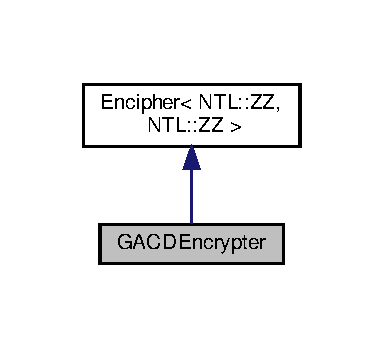
\includegraphics[width=184pt]{classGACDEncrypter__inherit__graph}
\end{center}
\end{figure}


Collaboration diagram for G\+A\+C\+D\+Encrypter\+:
\nopagebreak
\begin{figure}[H]
\begin{center}
\leavevmode
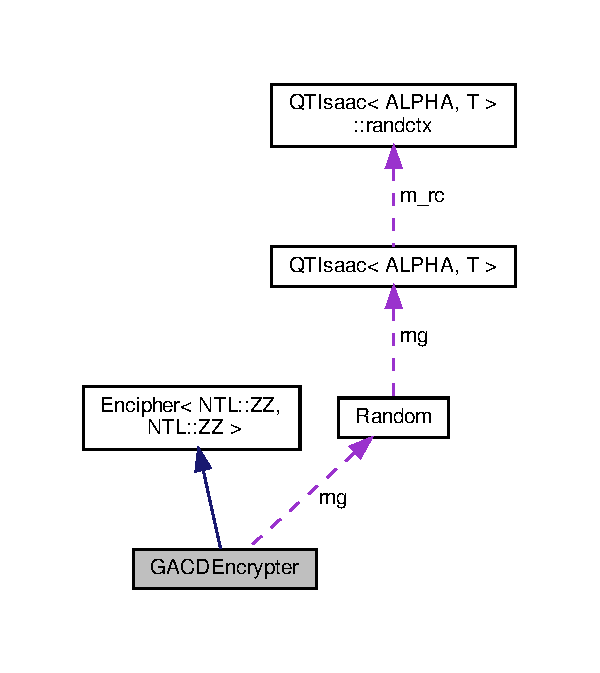
\includegraphics[width=288pt]{classGACDEncrypter__coll__graph}
\end{center}
\end{figure}
\subsection*{Public Member Functions}
\begin{DoxyCompactItemize}
\item 
\hyperlink{classGACDEncrypter_a923b16f668dca6e17857df7c825ab66f}{G\+A\+C\+D\+Encrypter} (int bits)
\item 
virtual \hyperlink{classGACDEncrypter_a9cccf9b5e5f8728c1df5c73cea492fca}{$\sim$\+G\+A\+C\+D\+Encrypter} ()
\item 
N\+T\+L\+::\+ZZ \hyperlink{classGACDEncrypter_a310a857f6b77a6c83d4319968d49902f}{encrypt} (N\+T\+L\+::\+ZZ \&plaintext) override
\item 
std\+::string \hyperlink{classGACDEncrypter_a01cd18ae81d0d28076c4ceb690a8b418}{write\+Secrets\+To\+J\+S\+ON} () override
\end{DoxyCompactItemize}
\subsection*{Private Attributes}
\begin{DoxyCompactItemize}
\item 
N\+T\+L\+::\+ZZ \hyperlink{classGACDEncrypter_af235b4e988a563f05d29b461c88f8703}{k}
\item 
N\+T\+L\+::\+ZZ \hyperlink{classGACDEncrypter_a6b0e9a07d27ec0976cc7958df6f666a4}{minr}
\item 
N\+T\+L\+::\+ZZ \hyperlink{classGACDEncrypter_a646b9daae82d6666d6a8affd3de41fd5}{maxr}
\item 
\hyperlink{classRandom}{Random} \hyperlink{classGACDEncrypter_a3f8959f045b15262ae7d680b35d0815c}{rng}
\end{DoxyCompactItemize}


\subsection{Constructor \& Destructor Documentation}
\mbox{\Hypertarget{classGACDEncrypter_a923b16f668dca6e17857df7c825ab66f}\label{classGACDEncrypter_a923b16f668dca6e17857df7c825ab66f}} 
\index{G\+A\+C\+D\+Encrypter@{G\+A\+C\+D\+Encrypter}!G\+A\+C\+D\+Encrypter@{G\+A\+C\+D\+Encrypter}}
\index{G\+A\+C\+D\+Encrypter@{G\+A\+C\+D\+Encrypter}!G\+A\+C\+D\+Encrypter@{G\+A\+C\+D\+Encrypter}}
\subsubsection{\texorpdfstring{G\+A\+C\+D\+Encrypter()}{GACDEncrypter()}}
{\footnotesize\ttfamily G\+A\+C\+D\+Encrypter\+::\+G\+A\+C\+D\+Encrypter (\begin{DoxyParamCaption}\item[{int}]{bits }\end{DoxyParamCaption})}

\mbox{\Hypertarget{classGACDEncrypter_a9cccf9b5e5f8728c1df5c73cea492fca}\label{classGACDEncrypter_a9cccf9b5e5f8728c1df5c73cea492fca}} 
\index{G\+A\+C\+D\+Encrypter@{G\+A\+C\+D\+Encrypter}!````~G\+A\+C\+D\+Encrypter@{$\sim$\+G\+A\+C\+D\+Encrypter}}
\index{````~G\+A\+C\+D\+Encrypter@{$\sim$\+G\+A\+C\+D\+Encrypter}!G\+A\+C\+D\+Encrypter@{G\+A\+C\+D\+Encrypter}}
\subsubsection{\texorpdfstring{$\sim$\+G\+A\+C\+D\+Encrypter()}{~GACDEncrypter()}}
{\footnotesize\ttfamily G\+A\+C\+D\+Encrypter\+::$\sim$\+G\+A\+C\+D\+Encrypter (\begin{DoxyParamCaption}{ }\end{DoxyParamCaption})\hspace{0.3cm}{\ttfamily [virtual]}}



\subsection{Member Function Documentation}
\mbox{\Hypertarget{classGACDEncrypter_a310a857f6b77a6c83d4319968d49902f}\label{classGACDEncrypter_a310a857f6b77a6c83d4319968d49902f}} 
\index{G\+A\+C\+D\+Encrypter@{G\+A\+C\+D\+Encrypter}!encrypt@{encrypt}}
\index{encrypt@{encrypt}!G\+A\+C\+D\+Encrypter@{G\+A\+C\+D\+Encrypter}}
\subsubsection{\texorpdfstring{encrypt()}{encrypt()}}
{\footnotesize\ttfamily N\+T\+L\+::\+ZZ G\+A\+C\+D\+Encrypter\+::encrypt (\begin{DoxyParamCaption}\item[{N\+T\+L\+::\+ZZ \&}]{plaintext }\end{DoxyParamCaption})\hspace{0.3cm}{\ttfamily [override]}, {\ttfamily [virtual]}}



Implements \hyperlink{classEncipher_aaf8138eb280608bfd03c6eb762ffc010}{Encipher$<$ N\+T\+L\+::\+Z\+Z, N\+T\+L\+::\+Z\+Z $>$}.

\mbox{\Hypertarget{classGACDEncrypter_a01cd18ae81d0d28076c4ceb690a8b418}\label{classGACDEncrypter_a01cd18ae81d0d28076c4ceb690a8b418}} 
\index{G\+A\+C\+D\+Encrypter@{G\+A\+C\+D\+Encrypter}!write\+Secrets\+To\+J\+S\+ON@{write\+Secrets\+To\+J\+S\+ON}}
\index{write\+Secrets\+To\+J\+S\+ON@{write\+Secrets\+To\+J\+S\+ON}!G\+A\+C\+D\+Encrypter@{G\+A\+C\+D\+Encrypter}}
\subsubsection{\texorpdfstring{write\+Secrets\+To\+J\+S\+O\+N()}{writeSecretsToJSON()}}
{\footnotesize\ttfamily std\+::string G\+A\+C\+D\+Encrypter\+::write\+Secrets\+To\+J\+S\+ON (\begin{DoxyParamCaption}{ }\end{DoxyParamCaption})\hspace{0.3cm}{\ttfamily [override]}, {\ttfamily [virtual]}}



Implements \hyperlink{classEncipher_a27d3efa1e364c1f0d7def65454c61b85}{Encipher$<$ N\+T\+L\+::\+Z\+Z, N\+T\+L\+::\+Z\+Z $>$}.



\subsection{Member Data Documentation}
\mbox{\Hypertarget{classGACDEncrypter_af235b4e988a563f05d29b461c88f8703}\label{classGACDEncrypter_af235b4e988a563f05d29b461c88f8703}} 
\index{G\+A\+C\+D\+Encrypter@{G\+A\+C\+D\+Encrypter}!k@{k}}
\index{k@{k}!G\+A\+C\+D\+Encrypter@{G\+A\+C\+D\+Encrypter}}
\subsubsection{\texorpdfstring{k}{k}}
{\footnotesize\ttfamily N\+T\+L\+::\+ZZ G\+A\+C\+D\+Encrypter\+::k\hspace{0.3cm}{\ttfamily [private]}}

\mbox{\Hypertarget{classGACDEncrypter_a646b9daae82d6666d6a8affd3de41fd5}\label{classGACDEncrypter_a646b9daae82d6666d6a8affd3de41fd5}} 
\index{G\+A\+C\+D\+Encrypter@{G\+A\+C\+D\+Encrypter}!maxr@{maxr}}
\index{maxr@{maxr}!G\+A\+C\+D\+Encrypter@{G\+A\+C\+D\+Encrypter}}
\subsubsection{\texorpdfstring{maxr}{maxr}}
{\footnotesize\ttfamily N\+T\+L\+::\+ZZ G\+A\+C\+D\+Encrypter\+::maxr\hspace{0.3cm}{\ttfamily [private]}}

\mbox{\Hypertarget{classGACDEncrypter_a6b0e9a07d27ec0976cc7958df6f666a4}\label{classGACDEncrypter_a6b0e9a07d27ec0976cc7958df6f666a4}} 
\index{G\+A\+C\+D\+Encrypter@{G\+A\+C\+D\+Encrypter}!minr@{minr}}
\index{minr@{minr}!G\+A\+C\+D\+Encrypter@{G\+A\+C\+D\+Encrypter}}
\subsubsection{\texorpdfstring{minr}{minr}}
{\footnotesize\ttfamily N\+T\+L\+::\+ZZ G\+A\+C\+D\+Encrypter\+::minr\hspace{0.3cm}{\ttfamily [private]}}

\mbox{\Hypertarget{classGACDEncrypter_a3f8959f045b15262ae7d680b35d0815c}\label{classGACDEncrypter_a3f8959f045b15262ae7d680b35d0815c}} 
\index{G\+A\+C\+D\+Encrypter@{G\+A\+C\+D\+Encrypter}!rng@{rng}}
\index{rng@{rng}!G\+A\+C\+D\+Encrypter@{G\+A\+C\+D\+Encrypter}}
\subsubsection{\texorpdfstring{rng}{rng}}
{\footnotesize\ttfamily \hyperlink{classRandom}{Random} G\+A\+C\+D\+Encrypter\+::rng\hspace{0.3cm}{\ttfamily [private]}}



The documentation for this class was generated from the following files\+:\begin{DoxyCompactItemize}
\item 
include/\hyperlink{GACDEncrypter_8h}{G\+A\+C\+D\+Encrypter.\+h}\item 
src/\hyperlink{GACDEncrypter_8cpp}{G\+A\+C\+D\+Encrypter.\+cpp}\end{DoxyCompactItemize}

\hypertarget{classHE1Decrypter}{}\section{H\+E1\+Decrypter Class Reference}
\label{classHE1Decrypter}\index{H\+E1\+Decrypter@{H\+E1\+Decrypter}}


{\ttfamily \#include $<$H\+E1\+Decrypter.\+h$>$}



Inheritance diagram for H\+E1\+Decrypter\+:\nopagebreak
\begin{figure}[H]
\begin{center}
\leavevmode
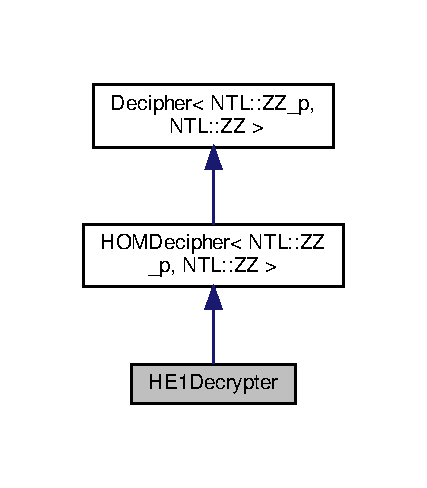
\includegraphics[width=205pt]{classHE1Decrypter__inherit__graph}
\end{center}
\end{figure}


Collaboration diagram for H\+E1\+Decrypter\+:\nopagebreak
\begin{figure}[H]
\begin{center}
\leavevmode
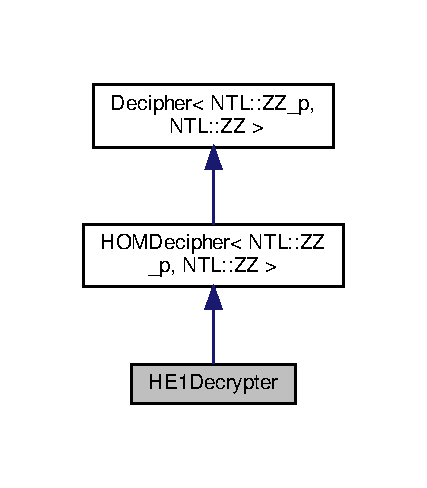
\includegraphics[width=205pt]{classHE1Decrypter__coll__graph}
\end{center}
\end{figure}
\subsection*{Public Member Functions}
\begin{DoxyCompactItemize}
\item 
void \hyperlink{classHE1Decrypter_af60ccc6d0afe7555a9d1468ad7047733}{read\+Secrets\+From\+J\+S\+ON} (std\+::string \&json) override
\item 
void \hyperlink{classHE1Decrypter_ab10c6ecc422cbf5f492c7a039e2da97c}{init} ()
\item 
N\+T\+L\+::\+ZZ \hyperlink{classHE1Decrypter_a28cc03e8a37f321b8f805cc04b2e69e0}{decrypt} (N\+T\+L\+::\+Z\+Z\+\_\+p \&ciphertext) override
\item 
void \hyperlink{classHE1Decrypter_a7b06b69bcd5ef096067232f819321482}{set\+Key} (N\+T\+L\+::\+ZZ \&key)
\item 
\hyperlink{classHE1Decrypter_a68c49940560941d85b53e1b8d8d20df1}{H\+E1\+Decrypter} ()
\item 
virtual \hyperlink{classHE1Decrypter_a9beb110e7544804f2c906bae64932aab}{$\sim$\+H\+E1\+Decrypter} ()
\end{DoxyCompactItemize}
\subsection*{Additional Inherited Members}


\subsection{Constructor \& Destructor Documentation}
\mbox{\Hypertarget{classHE1Decrypter_a68c49940560941d85b53e1b8d8d20df1}\label{classHE1Decrypter_a68c49940560941d85b53e1b8d8d20df1}} 
\index{H\+E1\+Decrypter@{H\+E1\+Decrypter}!H\+E1\+Decrypter@{H\+E1\+Decrypter}}
\index{H\+E1\+Decrypter@{H\+E1\+Decrypter}!H\+E1\+Decrypter@{H\+E1\+Decrypter}}
\subsubsection{\texorpdfstring{H\+E1\+Decrypter()}{HE1Decrypter()}}
{\footnotesize\ttfamily H\+E1\+Decrypter\+::\+H\+E1\+Decrypter (\begin{DoxyParamCaption}{ }\end{DoxyParamCaption})\hspace{0.3cm}{\ttfamily [inline]}}

\mbox{\Hypertarget{classHE1Decrypter_a9beb110e7544804f2c906bae64932aab}\label{classHE1Decrypter_a9beb110e7544804f2c906bae64932aab}} 
\index{H\+E1\+Decrypter@{H\+E1\+Decrypter}!````~H\+E1\+Decrypter@{$\sim$\+H\+E1\+Decrypter}}
\index{````~H\+E1\+Decrypter@{$\sim$\+H\+E1\+Decrypter}!H\+E1\+Decrypter@{H\+E1\+Decrypter}}
\subsubsection{\texorpdfstring{$\sim$\+H\+E1\+Decrypter()}{~HE1Decrypter()}}
{\footnotesize\ttfamily virtual H\+E1\+Decrypter\+::$\sim$\+H\+E1\+Decrypter (\begin{DoxyParamCaption}{ }\end{DoxyParamCaption})\hspace{0.3cm}{\ttfamily [inline]}, {\ttfamily [virtual]}}



\subsection{Member Function Documentation}
\mbox{\Hypertarget{classHE1Decrypter_a28cc03e8a37f321b8f805cc04b2e69e0}\label{classHE1Decrypter_a28cc03e8a37f321b8f805cc04b2e69e0}} 
\index{H\+E1\+Decrypter@{H\+E1\+Decrypter}!decrypt@{decrypt}}
\index{decrypt@{decrypt}!H\+E1\+Decrypter@{H\+E1\+Decrypter}}
\subsubsection{\texorpdfstring{decrypt()}{decrypt()}}
{\footnotesize\ttfamily N\+T\+L\+::\+ZZ H\+E1\+Decrypter\+::decrypt (\begin{DoxyParamCaption}\item[{N\+T\+L\+::\+Z\+Z\+\_\+p \&}]{ciphertext }\end{DoxyParamCaption})\hspace{0.3cm}{\ttfamily [override]}, {\ttfamily [virtual]}}

Decrypts a ciphertext 
\begin{DoxyParams}{Parameters}
{\em ciphertext} & Ciphertext value \\
\hline
\end{DoxyParams}
\begin{DoxyReturn}{Returns}
Plaintext value 
\end{DoxyReturn}


Implements \hyperlink{classDecipher_ac6b8c369eda2d7e17fa90cb594cf41b6}{Decipher$<$ N\+T\+L\+::\+Z\+Z\+\_\+p, N\+T\+L\+::\+Z\+Z $>$}.

\mbox{\Hypertarget{classHE1Decrypter_ab10c6ecc422cbf5f492c7a039e2da97c}\label{classHE1Decrypter_ab10c6ecc422cbf5f492c7a039e2da97c}} 
\index{H\+E1\+Decrypter@{H\+E1\+Decrypter}!init@{init}}
\index{init@{init}!H\+E1\+Decrypter@{H\+E1\+Decrypter}}
\subsubsection{\texorpdfstring{init()}{init()}}
{\footnotesize\ttfamily void H\+E1\+Decrypter\+::init (\begin{DoxyParamCaption}{ }\end{DoxyParamCaption})}

Intialise the cipher by setting the local modulus for arithmetic operations to {\ttfamily p} \mbox{\Hypertarget{classHE1Decrypter_af60ccc6d0afe7555a9d1468ad7047733}\label{classHE1Decrypter_af60ccc6d0afe7555a9d1468ad7047733}} 
\index{H\+E1\+Decrypter@{H\+E1\+Decrypter}!read\+Secrets\+From\+J\+S\+ON@{read\+Secrets\+From\+J\+S\+ON}}
\index{read\+Secrets\+From\+J\+S\+ON@{read\+Secrets\+From\+J\+S\+ON}!H\+E1\+Decrypter@{H\+E1\+Decrypter}}
\subsubsection{\texorpdfstring{read\+Secrets\+From\+J\+S\+O\+N()}{readSecretsFromJSON()}}
{\footnotesize\ttfamily void H\+E1\+Decrypter\+::read\+Secrets\+From\+J\+S\+ON (\begin{DoxyParamCaption}\item[{std\+::string \&}]{string }\end{DoxyParamCaption})\hspace{0.3cm}{\ttfamily [override]}, {\ttfamily [virtual]}}

Reads the cipher secrets in from a J\+S\+ON string 
\begin{DoxyParams}{Parameters}
{\em string} & J\+S\+ON string \\
\hline
\end{DoxyParams}


Implements \hyperlink{classDecipher_a39aea002012130201e12a8fa7d84dda5}{Decipher$<$ N\+T\+L\+::\+Z\+Z\+\_\+p, N\+T\+L\+::\+Z\+Z $>$}.

\mbox{\Hypertarget{classHE1Decrypter_a7b06b69bcd5ef096067232f819321482}\label{classHE1Decrypter_a7b06b69bcd5ef096067232f819321482}} 
\index{H\+E1\+Decrypter@{H\+E1\+Decrypter}!set\+Key@{set\+Key}}
\index{set\+Key@{set\+Key}!H\+E1\+Decrypter@{H\+E1\+Decrypter}}
\subsubsection{\texorpdfstring{set\+Key()}{setKey()}}
{\footnotesize\ttfamily void H\+E1\+Decrypter\+::set\+Key (\begin{DoxyParamCaption}\item[{N\+T\+L\+::\+ZZ \&}]{key }\end{DoxyParamCaption})}

Set the secret key to the given value 
\begin{DoxyParams}{Parameters}
{\em key} & Multiprecision integer \\
\hline
\end{DoxyParams}


The documentation for this class was generated from the following files\+:\begin{DoxyCompactItemize}
\item 
include/\hyperlink{HE1Decrypter_8h}{H\+E1\+Decrypter.\+h}\item 
src/\hyperlink{HE1Decrypter_8cpp}{H\+E1\+Decrypter.\+cpp}\end{DoxyCompactItemize}

\hypertarget{classHE1Encipher}{}\section{H\+E1\+Encipher Class Reference}
\label{classHE1Encipher}\index{H\+E1\+Encipher@{H\+E1\+Encipher}}


{\ttfamily \#include $<$H\+E1\+Encipher.\+h$>$}



Inheritance diagram for H\+E1\+Encipher\+:
\nopagebreak
\begin{figure}[H]
\begin{center}
\leavevmode
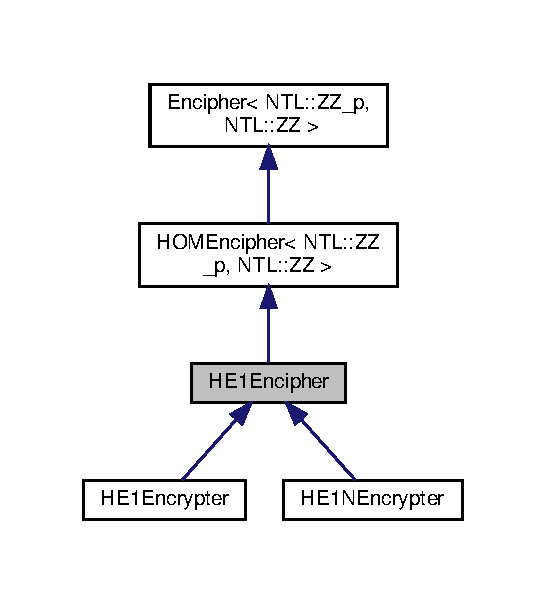
\includegraphics[width=262pt]{classHE1Encipher__inherit__graph}
\end{center}
\end{figure}


Collaboration diagram for H\+E1\+Encipher\+:
\nopagebreak
\begin{figure}[H]
\begin{center}
\leavevmode
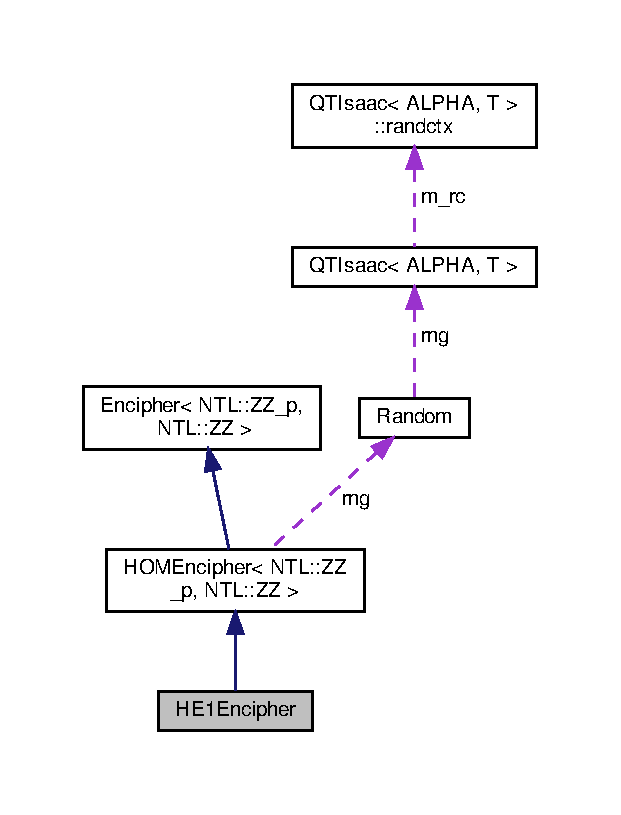
\includegraphics[width=298pt]{classHE1Encipher__coll__graph}
\end{center}
\end{figure}
\subsection*{Public Member Functions}
\begin{DoxyCompactItemize}
\item 
std\+::string \hyperlink{classHE1Encipher_a0aa1ef94d9147591367dbbc6ce03e5e1}{write\+Parameters\+To\+J\+S\+ON} () override
\item 
\hyperlink{classHE1Encipher_ad9128098166937e3569c4414aa1af689}{H\+E1\+Encipher} ()
\item 
virtual \hyperlink{classHE1Encipher_a5ffc18928bd189107151cb5a16c8cc5c}{$\sim$\+H\+E1\+Encipher} ()
\end{DoxyCompactItemize}
\subsection*{Static Public Attributes}
\begin{DoxyCompactItemize}
\item 
static N\+T\+L\+::\+ZZ \hyperlink{classHE1Encipher_a9c4f95a1461ec32d6e96db7c67aabdf3}{O\+NE} = N\+T\+L\+::\+ZZ(1)
\end{DoxyCompactItemize}
\subsection*{Protected Member Functions}
\begin{DoxyCompactItemize}
\item 
void \hyperlink{classHE1Encipher_a4ec1a767a1a3f4e71fa368dc99f6afd8}{generate\+Parameters} (long lambda, long eta)
\end{DoxyCompactItemize}
\subsection*{Protected Attributes}
\begin{DoxyCompactItemize}
\item 
N\+T\+L\+::\+Z\+Z\+\_\+p $\ast$ \hyperlink{classHE1Encipher_a4fa8ff49fc93cf01a0814aa83141e725}{pmod}
\end{DoxyCompactItemize}


\subsection{Constructor \& Destructor Documentation}
\mbox{\Hypertarget{classHE1Encipher_ad9128098166937e3569c4414aa1af689}\label{classHE1Encipher_ad9128098166937e3569c4414aa1af689}} 
\index{H\+E1\+Encipher@{H\+E1\+Encipher}!H\+E1\+Encipher@{H\+E1\+Encipher}}
\index{H\+E1\+Encipher@{H\+E1\+Encipher}!H\+E1\+Encipher@{H\+E1\+Encipher}}
\subsubsection{\texorpdfstring{H\+E1\+Encipher()}{HE1Encipher()}}
{\footnotesize\ttfamily H\+E1\+Encipher\+::\+H\+E1\+Encipher (\begin{DoxyParamCaption}{ }\end{DoxyParamCaption})}

\mbox{\Hypertarget{classHE1Encipher_a5ffc18928bd189107151cb5a16c8cc5c}\label{classHE1Encipher_a5ffc18928bd189107151cb5a16c8cc5c}} 
\index{H\+E1\+Encipher@{H\+E1\+Encipher}!````~H\+E1\+Encipher@{$\sim$\+H\+E1\+Encipher}}
\index{````~H\+E1\+Encipher@{$\sim$\+H\+E1\+Encipher}!H\+E1\+Encipher@{H\+E1\+Encipher}}
\subsubsection{\texorpdfstring{$\sim$\+H\+E1\+Encipher()}{~HE1Encipher()}}
{\footnotesize\ttfamily H\+E1\+Encipher\+::$\sim$\+H\+E1\+Encipher (\begin{DoxyParamCaption}{ }\end{DoxyParamCaption})\hspace{0.3cm}{\ttfamily [virtual]}}



\subsection{Member Function Documentation}
\mbox{\Hypertarget{classHE1Encipher_a4ec1a767a1a3f4e71fa368dc99f6afd8}\label{classHE1Encipher_a4ec1a767a1a3f4e71fa368dc99f6afd8}} 
\index{H\+E1\+Encipher@{H\+E1\+Encipher}!generate\+Parameters@{generate\+Parameters}}
\index{generate\+Parameters@{generate\+Parameters}!H\+E1\+Encipher@{H\+E1\+Encipher}}
\subsubsection{\texorpdfstring{generate\+Parameters()}{generateParameters()}}
{\footnotesize\ttfamily void H\+E1\+Encipher\+::generate\+Parameters (\begin{DoxyParamCaption}\item[{long}]{lambda,  }\item[{long}]{eta }\end{DoxyParamCaption})\hspace{0.3cm}{\ttfamily [protected]}}

\mbox{\Hypertarget{classHE1Encipher_a0aa1ef94d9147591367dbbc6ce03e5e1}\label{classHE1Encipher_a0aa1ef94d9147591367dbbc6ce03e5e1}} 
\index{H\+E1\+Encipher@{H\+E1\+Encipher}!write\+Parameters\+To\+J\+S\+ON@{write\+Parameters\+To\+J\+S\+ON}}
\index{write\+Parameters\+To\+J\+S\+ON@{write\+Parameters\+To\+J\+S\+ON}!H\+E1\+Encipher@{H\+E1\+Encipher}}
\subsubsection{\texorpdfstring{write\+Parameters\+To\+J\+S\+O\+N()}{writeParametersToJSON()}}
{\footnotesize\ttfamily std\+::string H\+E1\+Encipher\+::write\+Parameters\+To\+J\+S\+ON (\begin{DoxyParamCaption}{ }\end{DoxyParamCaption})\hspace{0.3cm}{\ttfamily [override]}, {\ttfamily [virtual]}}



Implements \hyperlink{classHOMEncipher_abf176e3fb85de6f0f6a2c96563397d39}{H\+O\+M\+Encipher$<$ N\+T\+L\+::\+Z\+Z\+\_\+p, N\+T\+L\+::\+Z\+Z $>$}.



\subsection{Member Data Documentation}
\mbox{\Hypertarget{classHE1Encipher_a9c4f95a1461ec32d6e96db7c67aabdf3}\label{classHE1Encipher_a9c4f95a1461ec32d6e96db7c67aabdf3}} 
\index{H\+E1\+Encipher@{H\+E1\+Encipher}!O\+NE@{O\+NE}}
\index{O\+NE@{O\+NE}!H\+E1\+Encipher@{H\+E1\+Encipher}}
\subsubsection{\texorpdfstring{O\+NE}{ONE}}
{\footnotesize\ttfamily N\+T\+L\+::\+ZZ H\+E1\+Encipher\+::\+O\+NE = N\+T\+L\+::\+ZZ(1)\hspace{0.3cm}{\ttfamily [static]}}

\mbox{\Hypertarget{classHE1Encipher_a4fa8ff49fc93cf01a0814aa83141e725}\label{classHE1Encipher_a4fa8ff49fc93cf01a0814aa83141e725}} 
\index{H\+E1\+Encipher@{H\+E1\+Encipher}!pmod@{pmod}}
\index{pmod@{pmod}!H\+E1\+Encipher@{H\+E1\+Encipher}}
\subsubsection{\texorpdfstring{pmod}{pmod}}
{\footnotesize\ttfamily N\+T\+L\+::\+Z\+Z\+\_\+p$\ast$ H\+E1\+Encipher\+::pmod\hspace{0.3cm}{\ttfamily [protected]}}



The documentation for this class was generated from the following files\+:\begin{DoxyCompactItemize}
\item 
include/\hyperlink{HE1Encipher_8h}{H\+E1\+Encipher.\+h}\item 
src/\hyperlink{HE1Encipher_8cpp}{H\+E1\+Encipher.\+cpp}\end{DoxyCompactItemize}

\hypertarget{classHE1Encrypter}{}\section{H\+E1\+Encrypter Class Reference}
\label{classHE1Encrypter}\index{H\+E1\+Encrypter@{H\+E1\+Encrypter}}


{\ttfamily \#include $<$H\+E1\+Encrypter.\+h$>$}



Inheritance diagram for H\+E1\+Encrypter\+:\nopagebreak
\begin{figure}[H]
\begin{center}
\leavevmode
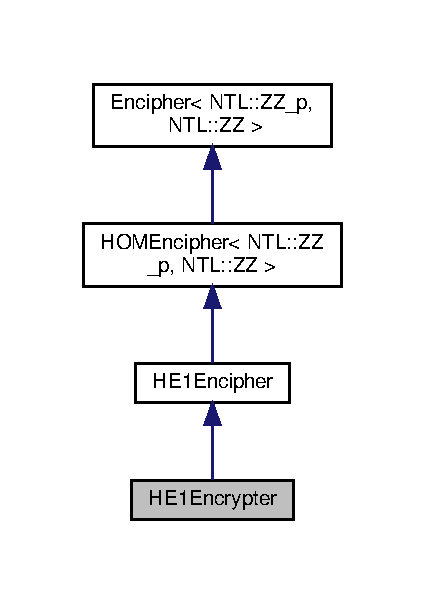
\includegraphics[width=204pt]{classHE1Encrypter__inherit__graph}
\end{center}
\end{figure}


Collaboration diagram for H\+E1\+Encrypter\+:\nopagebreak
\begin{figure}[H]
\begin{center}
\leavevmode
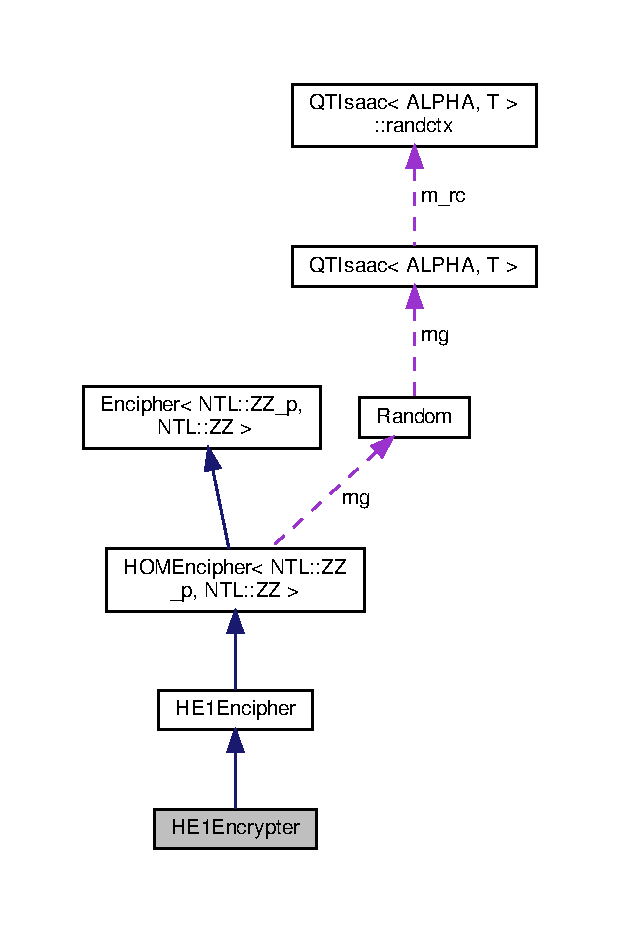
\includegraphics[width=298pt]{classHE1Encrypter__coll__graph}
\end{center}
\end{figure}
\subsection*{Public Member Functions}
\begin{DoxyCompactItemize}
\item 
N\+T\+L\+::\+Z\+Z\+\_\+p \hyperlink{classHE1Encrypter_afc178d8e27a1263bef824bfc8960dbc0}{encrypt} (N\+T\+L\+::\+ZZ \&plaintext) override
\item 
N\+T\+L\+::\+ZZ \& \hyperlink{classHE1Encrypter_a014c9eca9d9979fa45dad79b355a95cc}{get\+Key} ()
\item 
std\+::string \hyperlink{classHE1Encrypter_a05627c66faf89c133a24fa7bb4553ef2}{write\+Secrets\+To\+J\+S\+ON} () override
\item 
\hyperlink{classHE1Encrypter_a4126c0700e63763f7f239876a2196f54}{H\+E1\+Encrypter} (int lambda, int eta)
\item 
\hyperlink{classHE1Encrypter_a3cce07a63783a523afcf6905e2df4b93}{H\+E1\+Encrypter} (int n, int d, int rho)
\item 
virtual \hyperlink{classHE1Encrypter_ae9419b3ea61b96731501a9979f878131}{$\sim$\+H\+E1\+Encrypter} ()
\end{DoxyCompactItemize}
\subsection*{Additional Inherited Members}


\subsection{Constructor \& Destructor Documentation}
\mbox{\Hypertarget{classHE1Encrypter_a4126c0700e63763f7f239876a2196f54}\label{classHE1Encrypter_a4126c0700e63763f7f239876a2196f54}} 
\index{H\+E1\+Encrypter@{H\+E1\+Encrypter}!H\+E1\+Encrypter@{H\+E1\+Encrypter}}
\index{H\+E1\+Encrypter@{H\+E1\+Encrypter}!H\+E1\+Encrypter@{H\+E1\+Encrypter}}
\subsubsection{\texorpdfstring{H\+E1\+Encrypter()}{HE1Encrypter()}\hspace{0.1cm}{\footnotesize\ttfamily [1/2]}}
{\footnotesize\ttfamily H\+E1\+Encrypter\+::\+H\+E1\+Encrypter (\begin{DoxyParamCaption}\item[{int}]{lambda,  }\item[{int}]{eta }\end{DoxyParamCaption})}

Initialise cipher by generating cipher parameters such that {\ttfamily p} is a {\ttfamily lambda} bit prime and {\ttfamily q} is an {\ttfamily eta} bit prime. The public modulus for arithmetic operations on ciphertexts is {\ttfamily pq} 
\begin{DoxyParams}{Parameters}
{\em lambda} & Bit length of secret modulus {\ttfamily p} (security parameter) \\
\hline
{\em eta} & Bit length of secret prime {\ttfamily q}. \\
\hline
\end{DoxyParams}
\mbox{\Hypertarget{classHE1Encrypter_a3cce07a63783a523afcf6905e2df4b93}\label{classHE1Encrypter_a3cce07a63783a523afcf6905e2df4b93}} 
\index{H\+E1\+Encrypter@{H\+E1\+Encrypter}!H\+E1\+Encrypter@{H\+E1\+Encrypter}}
\index{H\+E1\+Encrypter@{H\+E1\+Encrypter}!H\+E1\+Encrypter@{H\+E1\+Encrypter}}
\subsubsection{\texorpdfstring{H\+E1\+Encrypter()}{HE1Encrypter()}\hspace{0.1cm}{\footnotesize\ttfamily [2/2]}}
{\footnotesize\ttfamily H\+E1\+Encrypter\+::\+H\+E1\+Encrypter (\begin{DoxyParamCaption}\item[{int}]{n,  }\item[{int}]{d,  }\item[{int}]{rho }\end{DoxyParamCaption})}

Initialise cipher by generating cipher parameters so that {\ttfamily p} is large enough to accommodate a degree {\ttfamily d} multivariate polynomial computed over {\ttfamily n} {\ttfamily rho\%-\/bit} integer inputs and {\ttfamily q} is large enough so that {\ttfamily pq} cannot be factored in polynomial time. 
\begin{DoxyParams}{Parameters}
{\em n} & total number of inputs \\
\hline
{\em d} & degree of polynomial to compute \\
\hline
{\em rho} & bit length of inputs, e.\+g for 32-\/bit integers {\ttfamily rho} = 32 \\
\hline
\end{DoxyParams}
\mbox{\Hypertarget{classHE1Encrypter_ae9419b3ea61b96731501a9979f878131}\label{classHE1Encrypter_ae9419b3ea61b96731501a9979f878131}} 
\index{H\+E1\+Encrypter@{H\+E1\+Encrypter}!````~H\+E1\+Encrypter@{$\sim$\+H\+E1\+Encrypter}}
\index{````~H\+E1\+Encrypter@{$\sim$\+H\+E1\+Encrypter}!H\+E1\+Encrypter@{H\+E1\+Encrypter}}
\subsubsection{\texorpdfstring{$\sim$\+H\+E1\+Encrypter()}{~HE1Encrypter()}}
{\footnotesize\ttfamily virtual H\+E1\+Encrypter\+::$\sim$\+H\+E1\+Encrypter (\begin{DoxyParamCaption}{ }\end{DoxyParamCaption})\hspace{0.3cm}{\ttfamily [virtual]}}



\subsection{Member Function Documentation}
\mbox{\Hypertarget{classHE1Encrypter_afc178d8e27a1263bef824bfc8960dbc0}\label{classHE1Encrypter_afc178d8e27a1263bef824bfc8960dbc0}} 
\index{H\+E1\+Encrypter@{H\+E1\+Encrypter}!encrypt@{encrypt}}
\index{encrypt@{encrypt}!H\+E1\+Encrypter@{H\+E1\+Encrypter}}
\subsubsection{\texorpdfstring{encrypt()}{encrypt()}}
{\footnotesize\ttfamily N\+T\+L\+::\+Z\+Z\+\_\+p H\+E1\+Encrypter\+::encrypt (\begin{DoxyParamCaption}\item[{N\+T\+L\+::\+ZZ \&}]{plaintext }\end{DoxyParamCaption})\hspace{0.3cm}{\ttfamily [override]}, {\ttfamily [virtual]}}

Encrypt a plaintext 
\begin{DoxyParams}{Parameters}
{\em plaintext} & A plaintext value \\
\hline
\end{DoxyParams}
\begin{DoxyReturn}{Returns}
A ciphertext value 
\end{DoxyReturn}


Implements \hyperlink{classEncipher_aaf8138eb280608bfd03c6eb762ffc010}{Encipher$<$ N\+T\+L\+::\+Z\+Z\+\_\+p, N\+T\+L\+::\+Z\+Z $>$}.

\mbox{\Hypertarget{classHE1Encrypter_a014c9eca9d9979fa45dad79b355a95cc}\label{classHE1Encrypter_a014c9eca9d9979fa45dad79b355a95cc}} 
\index{H\+E1\+Encrypter@{H\+E1\+Encrypter}!get\+Key@{get\+Key}}
\index{get\+Key@{get\+Key}!H\+E1\+Encrypter@{H\+E1\+Encrypter}}
\subsubsection{\texorpdfstring{get\+Key()}{getKey()}}
{\footnotesize\ttfamily N\+T\+L\+::\+ZZ \& H\+E1\+Encrypter\+::get\+Key (\begin{DoxyParamCaption}{ }\end{DoxyParamCaption})}

Accessor to retrieve the secret modulus, {\ttfamily p} \begin{DoxyReturn}{Returns}
Secret modulus {\ttfamily p} 
\end{DoxyReturn}
\mbox{\Hypertarget{classHE1Encrypter_a05627c66faf89c133a24fa7bb4553ef2}\label{classHE1Encrypter_a05627c66faf89c133a24fa7bb4553ef2}} 
\index{H\+E1\+Encrypter@{H\+E1\+Encrypter}!write\+Secrets\+To\+J\+S\+ON@{write\+Secrets\+To\+J\+S\+ON}}
\index{write\+Secrets\+To\+J\+S\+ON@{write\+Secrets\+To\+J\+S\+ON}!H\+E1\+Encrypter@{H\+E1\+Encrypter}}
\subsubsection{\texorpdfstring{write\+Secrets\+To\+J\+S\+O\+N()}{writeSecretsToJSON()}}
{\footnotesize\ttfamily std\+::string H\+E1\+Encrypter\+::write\+Secrets\+To\+J\+S\+ON (\begin{DoxyParamCaption}{ }\end{DoxyParamCaption})\hspace{0.3cm}{\ttfamily [override]}, {\ttfamily [virtual]}}

Writes cipher secrets out to a J\+S\+ON string \begin{DoxyReturn}{Returns}
J\+S\+ON string 
\end{DoxyReturn}


Implements \hyperlink{classEncipher_a27d3efa1e364c1f0d7def65454c61b85}{Encipher$<$ N\+T\+L\+::\+Z\+Z\+\_\+p, N\+T\+L\+::\+Z\+Z $>$}.



The documentation for this class was generated from the following files\+:\begin{DoxyCompactItemize}
\item 
include/\hyperlink{HE1Encrypter_8h}{H\+E1\+Encrypter.\+h}\item 
src/\hyperlink{HE1Encrypter_8cpp}{H\+E1\+Encrypter.\+cpp}\end{DoxyCompactItemize}

\hypertarget{classHE1NDecrypter}{}\section{H\+E1\+N\+Decrypter Class Reference}
\label{classHE1NDecrypter}\index{H\+E1\+N\+Decrypter@{H\+E1\+N\+Decrypter}}


{\ttfamily \#include $<$H\+E1\+N\+Decrypter.\+h$>$}



Inheritance diagram for H\+E1\+N\+Decrypter\+:\nopagebreak
\begin{figure}[H]
\begin{center}
\leavevmode
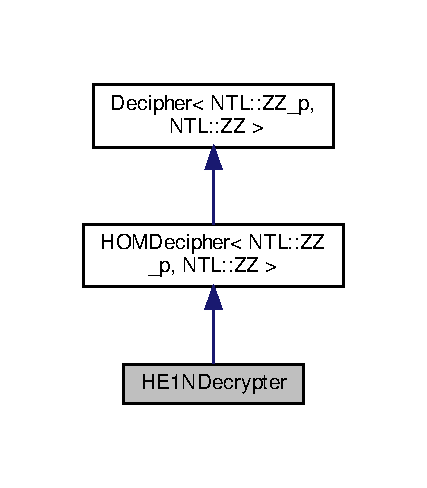
\includegraphics[width=205pt]{classHE1NDecrypter__inherit__graph}
\end{center}
\end{figure}


Collaboration diagram for H\+E1\+N\+Decrypter\+:\nopagebreak
\begin{figure}[H]
\begin{center}
\leavevmode
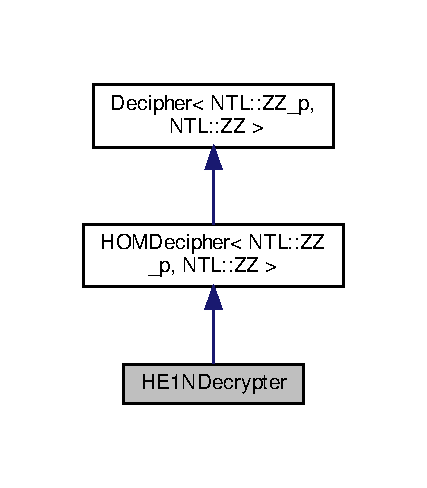
\includegraphics[width=205pt]{classHE1NDecrypter__coll__graph}
\end{center}
\end{figure}
\subsection*{Public Member Functions}
\begin{DoxyCompactItemize}
\item 
void \hyperlink{classHE1NDecrypter_a35a7d0c2ce869f417d6dc90792e61e11}{set\+Key} (N\+T\+L\+::vec\+\_\+\+ZZ \&key)
\item 
void \hyperlink{classHE1NDecrypter_a323f074a37cb4ebfbcfca4b6bdfb6737}{read\+Secrets\+From\+J\+S\+ON} (std\+::string \&json) override
\item 
N\+T\+L\+::\+ZZ \hyperlink{classHE1NDecrypter_a8e49ff8292a76884f328c566f4d1b646}{decrypt} (N\+T\+L\+::\+Z\+Z\+\_\+p \&ciphertext) override
\item 
\hyperlink{classHE1NDecrypter_a4aa5f1ecf0f7e0dcc3ea6e0073ac5e3a}{H\+E1\+N\+Decrypter} ()
\item 
virtual \hyperlink{classHE1NDecrypter_ae9d3f1b8d0012b99d12d24c0cc69d87e}{$\sim$\+H\+E1\+N\+Decrypter} ()
\end{DoxyCompactItemize}
\subsection*{Private Attributes}
\begin{DoxyCompactItemize}
\item 
N\+T\+L\+::\+ZZ \hyperlink{classHE1NDecrypter_a409fafa4eaf8d73998d6fee08ce4a8e2}{kappa}
\end{DoxyCompactItemize}
\subsection*{Additional Inherited Members}


\subsection{Constructor \& Destructor Documentation}
\mbox{\Hypertarget{classHE1NDecrypter_a4aa5f1ecf0f7e0dcc3ea6e0073ac5e3a}\label{classHE1NDecrypter_a4aa5f1ecf0f7e0dcc3ea6e0073ac5e3a}} 
\index{H\+E1\+N\+Decrypter@{H\+E1\+N\+Decrypter}!H\+E1\+N\+Decrypter@{H\+E1\+N\+Decrypter}}
\index{H\+E1\+N\+Decrypter@{H\+E1\+N\+Decrypter}!H\+E1\+N\+Decrypter@{H\+E1\+N\+Decrypter}}
\subsubsection{\texorpdfstring{H\+E1\+N\+Decrypter()}{HE1NDecrypter()}}
{\footnotesize\ttfamily H\+E1\+N\+Decrypter\+::\+H\+E1\+N\+Decrypter (\begin{DoxyParamCaption}{ }\end{DoxyParamCaption})\hspace{0.3cm}{\ttfamily [inline]}}

\mbox{\Hypertarget{classHE1NDecrypter_ae9d3f1b8d0012b99d12d24c0cc69d87e}\label{classHE1NDecrypter_ae9d3f1b8d0012b99d12d24c0cc69d87e}} 
\index{H\+E1\+N\+Decrypter@{H\+E1\+N\+Decrypter}!````~H\+E1\+N\+Decrypter@{$\sim$\+H\+E1\+N\+Decrypter}}
\index{````~H\+E1\+N\+Decrypter@{$\sim$\+H\+E1\+N\+Decrypter}!H\+E1\+N\+Decrypter@{H\+E1\+N\+Decrypter}}
\subsubsection{\texorpdfstring{$\sim$\+H\+E1\+N\+Decrypter()}{~HE1NDecrypter()}}
{\footnotesize\ttfamily virtual H\+E1\+N\+Decrypter\+::$\sim$\+H\+E1\+N\+Decrypter (\begin{DoxyParamCaption}{ }\end{DoxyParamCaption})\hspace{0.3cm}{\ttfamily [inline]}, {\ttfamily [virtual]}}



\subsection{Member Function Documentation}
\mbox{\Hypertarget{classHE1NDecrypter_a8e49ff8292a76884f328c566f4d1b646}\label{classHE1NDecrypter_a8e49ff8292a76884f328c566f4d1b646}} 
\index{H\+E1\+N\+Decrypter@{H\+E1\+N\+Decrypter}!decrypt@{decrypt}}
\index{decrypt@{decrypt}!H\+E1\+N\+Decrypter@{H\+E1\+N\+Decrypter}}
\subsubsection{\texorpdfstring{decrypt()}{decrypt()}}
{\footnotesize\ttfamily N\+T\+L\+::\+ZZ H\+E1\+N\+Decrypter\+::decrypt (\begin{DoxyParamCaption}\item[{N\+T\+L\+::\+Z\+Z\+\_\+p \&}]{ciphertext }\end{DoxyParamCaption})\hspace{0.3cm}{\ttfamily [override]}, {\ttfamily [virtual]}}

Decrypts a ciphertext 
\begin{DoxyParams}{Parameters}
{\em ciphertext} & Ciphertext value \\
\hline
\end{DoxyParams}
\begin{DoxyReturn}{Returns}
Plaintext value 
\end{DoxyReturn}


Implements \hyperlink{classDecipher_ac6b8c369eda2d7e17fa90cb594cf41b6}{Decipher$<$ N\+T\+L\+::\+Z\+Z\+\_\+p, N\+T\+L\+::\+Z\+Z $>$}.

\mbox{\Hypertarget{classHE1NDecrypter_a323f074a37cb4ebfbcfca4b6bdfb6737}\label{classHE1NDecrypter_a323f074a37cb4ebfbcfca4b6bdfb6737}} 
\index{H\+E1\+N\+Decrypter@{H\+E1\+N\+Decrypter}!read\+Secrets\+From\+J\+S\+ON@{read\+Secrets\+From\+J\+S\+ON}}
\index{read\+Secrets\+From\+J\+S\+ON@{read\+Secrets\+From\+J\+S\+ON}!H\+E1\+N\+Decrypter@{H\+E1\+N\+Decrypter}}
\subsubsection{\texorpdfstring{read\+Secrets\+From\+J\+S\+O\+N()}{readSecretsFromJSON()}}
{\footnotesize\ttfamily void H\+E1\+N\+Decrypter\+::read\+Secrets\+From\+J\+S\+ON (\begin{DoxyParamCaption}\item[{std\+::string \&}]{string }\end{DoxyParamCaption})\hspace{0.3cm}{\ttfamily [override]}, {\ttfamily [virtual]}}

Reads the cipher secrets in from a J\+S\+ON string 
\begin{DoxyParams}{Parameters}
{\em string} & J\+S\+ON string \\
\hline
\end{DoxyParams}


Implements \hyperlink{classDecipher_a39aea002012130201e12a8fa7d84dda5}{Decipher$<$ N\+T\+L\+::\+Z\+Z\+\_\+p, N\+T\+L\+::\+Z\+Z $>$}.

\mbox{\Hypertarget{classHE1NDecrypter_a35a7d0c2ce869f417d6dc90792e61e11}\label{classHE1NDecrypter_a35a7d0c2ce869f417d6dc90792e61e11}} 
\index{H\+E1\+N\+Decrypter@{H\+E1\+N\+Decrypter}!set\+Key@{set\+Key}}
\index{set\+Key@{set\+Key}!H\+E1\+N\+Decrypter@{H\+E1\+N\+Decrypter}}
\subsubsection{\texorpdfstring{set\+Key()}{setKey()}}
{\footnotesize\ttfamily void H\+E1\+N\+Decrypter\+::set\+Key (\begin{DoxyParamCaption}\item[{N\+T\+L\+::vec\+\_\+\+ZZ \&}]{key }\end{DoxyParamCaption})}

Set the secret parameters {\ttfamily p} and {\ttfamily kappa} from the given vector. 
\begin{DoxyParams}{Parameters}
{\em key} & A vector \\
\hline
\end{DoxyParams}


\subsection{Member Data Documentation}
\mbox{\Hypertarget{classHE1NDecrypter_a409fafa4eaf8d73998d6fee08ce4a8e2}\label{classHE1NDecrypter_a409fafa4eaf8d73998d6fee08ce4a8e2}} 
\index{H\+E1\+N\+Decrypter@{H\+E1\+N\+Decrypter}!kappa@{kappa}}
\index{kappa@{kappa}!H\+E1\+N\+Decrypter@{H\+E1\+N\+Decrypter}}
\subsubsection{\texorpdfstring{kappa}{kappa}}
{\footnotesize\ttfamily N\+T\+L\+::\+ZZ H\+E1\+N\+Decrypter\+::kappa\hspace{0.3cm}{\ttfamily [private]}}

A secret cipher parameter 

The documentation for this class was generated from the following files\+:\begin{DoxyCompactItemize}
\item 
include/\hyperlink{HE1NDecrypter_8h}{H\+E1\+N\+Decrypter.\+h}\item 
src/\hyperlink{HE1NDecrypter_8cpp}{H\+E1\+N\+Decrypter.\+cpp}\end{DoxyCompactItemize}

\hypertarget{classHE1NEncrypter}{}\section{H\+E1\+N\+Encrypter Class Reference}
\label{classHE1NEncrypter}\index{H\+E1\+N\+Encrypter@{H\+E1\+N\+Encrypter}}


{\ttfamily \#include $<$H\+E1\+N\+Encrypter.\+h$>$}



Inheritance diagram for H\+E1\+N\+Encrypter\+:\nopagebreak
\begin{figure}[H]
\begin{center}
\leavevmode
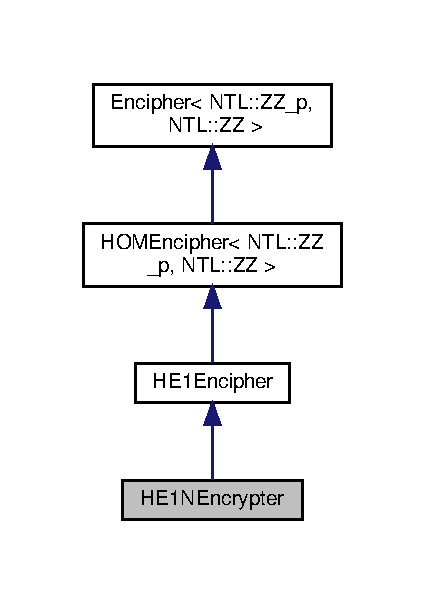
\includegraphics[width=204pt]{classHE1NEncrypter__inherit__graph}
\end{center}
\end{figure}


Collaboration diagram for H\+E1\+N\+Encrypter\+:\nopagebreak
\begin{figure}[H]
\begin{center}
\leavevmode
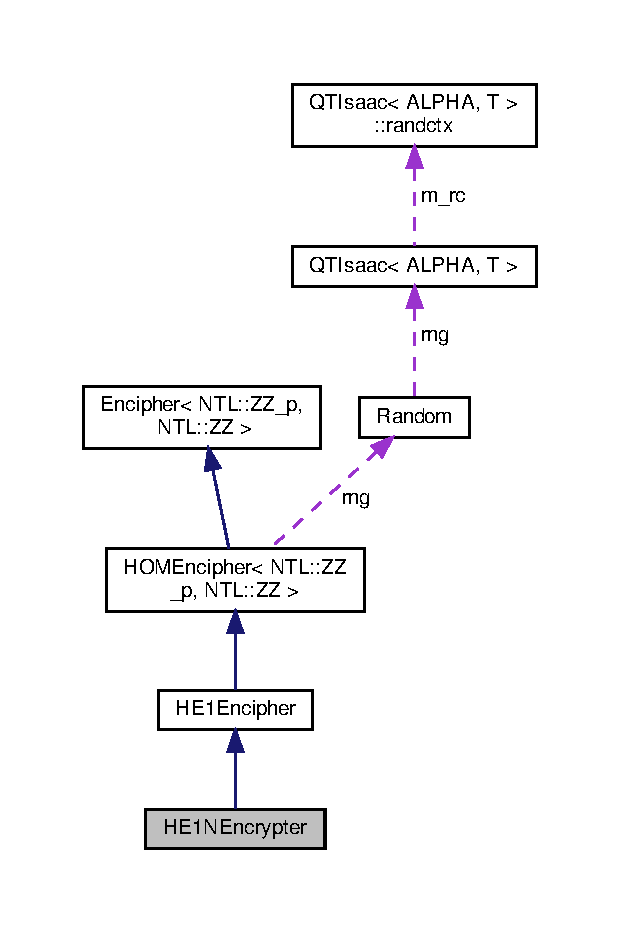
\includegraphics[width=298pt]{classHE1NEncrypter__coll__graph}
\end{center}
\end{figure}
\subsection*{Public Member Functions}
\begin{DoxyCompactItemize}
\item 
N\+T\+L\+::vec\+\_\+\+ZZ \hyperlink{classHE1NEncrypter_a68735a56be50d13e04824e48a61fc2f8}{get\+Key} ()
\item 
N\+T\+L\+::\+Z\+Z\+\_\+p \hyperlink{classHE1NEncrypter_a9a9c76558466ac56093cb6da937c7fe3}{encrypt} (N\+T\+L\+::\+ZZ \&plaintext) override
\item 
std\+::string \hyperlink{classHE1NEncrypter_ad1bca3e0933b8e15b91d208e421f83b2}{write\+Secrets\+To\+J\+S\+ON} () override
\item 
\hyperlink{classHE1NEncrypter_ac8b2f33fc7d1cba481944b16072efab0}{H\+E1\+N\+Encrypter} (int lambda, int eta, int nu)
\item 
\hyperlink{classHE1NEncrypter_a744ec5a8d26d1877114d6bd679a9e9ed}{H\+E1\+N\+Encrypter} (int n, int d, int rho, int rhoprime)
\item 
\hyperlink{classHE1NEncrypter_ac8eae729be42e97261e0387540699b75}{H\+E1\+N\+Encrypter} (std\+::string \&secrets, std\+::string \&parameters)
\item 
virtual \hyperlink{classHE1NEncrypter_a995b560b8ae6270eb325b52b0073e86b}{$\sim$\+H\+E1\+N\+Encrypter} ()
\end{DoxyCompactItemize}
\subsection*{Private Attributes}
\begin{DoxyCompactItemize}
\item 
N\+T\+L\+::\+ZZ \hyperlink{classHE1NEncrypter_a6ae3f5e69318587ba70afc87d21e6e11}{kappa}
\item 
N\+T\+L\+::\+Z\+Z\+\_\+p $\ast$ \hyperlink{classHE1NEncrypter_ae878596c30bc5825c3366366bf2b07fc}{kappamod}
\end{DoxyCompactItemize}
\subsection*{Additional Inherited Members}


\subsection{Constructor \& Destructor Documentation}
\mbox{\Hypertarget{classHE1NEncrypter_ac8b2f33fc7d1cba481944b16072efab0}\label{classHE1NEncrypter_ac8b2f33fc7d1cba481944b16072efab0}} 
\index{H\+E1\+N\+Encrypter@{H\+E1\+N\+Encrypter}!H\+E1\+N\+Encrypter@{H\+E1\+N\+Encrypter}}
\index{H\+E1\+N\+Encrypter@{H\+E1\+N\+Encrypter}!H\+E1\+N\+Encrypter@{H\+E1\+N\+Encrypter}}
\subsubsection{\texorpdfstring{H\+E1\+N\+Encrypter()}{HE1NEncrypter()}\hspace{0.1cm}{\footnotesize\ttfamily [1/3]}}
{\footnotesize\ttfamily H\+E1\+N\+Encrypter\+::\+H\+E1\+N\+Encrypter (\begin{DoxyParamCaption}\item[{int}]{lambda,  }\item[{int}]{eta,  }\item[{int}]{nu }\end{DoxyParamCaption})}

Initialise cipher by generating cipher parameters such that {\ttfamily p} is a {\ttfamily lambda} bit prime, {\ttfamily q} is an {\ttfamily eta} bit prime, and {\ttfamily kappa} is a {\ttfamily nu} bit prime. The public modulus for arithmetic operations on ciphertexts is {\ttfamily pq} 
\begin{DoxyParams}{Parameters}
{\em lambda} & Bit length of secret modulus {\ttfamily p} (security parameter) \\
\hline
{\em eta} & Bit length of secret prime {\ttfamily q} \\
\hline
{\em nu} & Bit length of secret prime {\ttfamily kappa}. \\
\hline
\end{DoxyParams}
\mbox{\Hypertarget{classHE1NEncrypter_a744ec5a8d26d1877114d6bd679a9e9ed}\label{classHE1NEncrypter_a744ec5a8d26d1877114d6bd679a9e9ed}} 
\index{H\+E1\+N\+Encrypter@{H\+E1\+N\+Encrypter}!H\+E1\+N\+Encrypter@{H\+E1\+N\+Encrypter}}
\index{H\+E1\+N\+Encrypter@{H\+E1\+N\+Encrypter}!H\+E1\+N\+Encrypter@{H\+E1\+N\+Encrypter}}
\subsubsection{\texorpdfstring{H\+E1\+N\+Encrypter()}{HE1NEncrypter()}\hspace{0.1cm}{\footnotesize\ttfamily [2/3]}}
{\footnotesize\ttfamily H\+E1\+N\+Encrypter\+::\+H\+E1\+N\+Encrypter (\begin{DoxyParamCaption}\item[{int}]{n,  }\item[{int}]{d,  }\item[{int}]{rho,  }\item[{int}]{rhoprime }\end{DoxyParamCaption})}

Initialise cipher by generating cipher parameters so that {\ttfamily p} and {\ttfamily kappa} are large enough to accommodate a degree {\ttfamily d} multivariate polynomial computed over {\ttfamily n} {\ttfamily rhoprime\%-\/bit} integers and {\ttfamily q} is large enough so that {\ttfamily pq} cannot be factored in polynomial time. 
\begin{DoxyParams}{Parameters}
{\em n} & total number of inputs \\
\hline
{\em d} & degree of polynomial to compute \\
\hline
{\em rho} & bit length of inputs, e.\+g for 32-\/bit integers {\ttfamily rho} = 32 \\
\hline
{\em rhoprime} & The effective entropy (bit lengths) of the inputs after encryption. \\
\hline
\end{DoxyParams}
\mbox{\Hypertarget{classHE1NEncrypter_ac8eae729be42e97261e0387540699b75}\label{classHE1NEncrypter_ac8eae729be42e97261e0387540699b75}} 
\index{H\+E1\+N\+Encrypter@{H\+E1\+N\+Encrypter}!H\+E1\+N\+Encrypter@{H\+E1\+N\+Encrypter}}
\index{H\+E1\+N\+Encrypter@{H\+E1\+N\+Encrypter}!H\+E1\+N\+Encrypter@{H\+E1\+N\+Encrypter}}
\subsubsection{\texorpdfstring{H\+E1\+N\+Encrypter()}{HE1NEncrypter()}\hspace{0.1cm}{\footnotesize\ttfamily [3/3]}}
{\footnotesize\ttfamily H\+E1\+N\+Encrypter\+::\+H\+E1\+N\+Encrypter (\begin{DoxyParamCaption}\item[{std\+::string \&}]{secrets,  }\item[{std\+::string \&}]{parameters }\end{DoxyParamCaption})}

Initialises the cipher using pre-\/existing cipher secrets and parameters 
\begin{DoxyParams}{Parameters}
{\em secrets} & A J\+S\+ON string \\
\hline
{\em parameters} & A J\+S\+ON string \\
\hline
\end{DoxyParams}
\mbox{\Hypertarget{classHE1NEncrypter_a995b560b8ae6270eb325b52b0073e86b}\label{classHE1NEncrypter_a995b560b8ae6270eb325b52b0073e86b}} 
\index{H\+E1\+N\+Encrypter@{H\+E1\+N\+Encrypter}!````~H\+E1\+N\+Encrypter@{$\sim$\+H\+E1\+N\+Encrypter}}
\index{````~H\+E1\+N\+Encrypter@{$\sim$\+H\+E1\+N\+Encrypter}!H\+E1\+N\+Encrypter@{H\+E1\+N\+Encrypter}}
\subsubsection{\texorpdfstring{$\sim$\+H\+E1\+N\+Encrypter()}{~HE1NEncrypter()}}
{\footnotesize\ttfamily H\+E1\+N\+Encrypter\+::$\sim$\+H\+E1\+N\+Encrypter (\begin{DoxyParamCaption}{ }\end{DoxyParamCaption})\hspace{0.3cm}{\ttfamily [virtual]}}

Default destructor 

\subsection{Member Function Documentation}
\mbox{\Hypertarget{classHE1NEncrypter_a9a9c76558466ac56093cb6da937c7fe3}\label{classHE1NEncrypter_a9a9c76558466ac56093cb6da937c7fe3}} 
\index{H\+E1\+N\+Encrypter@{H\+E1\+N\+Encrypter}!encrypt@{encrypt}}
\index{encrypt@{encrypt}!H\+E1\+N\+Encrypter@{H\+E1\+N\+Encrypter}}
\subsubsection{\texorpdfstring{encrypt()}{encrypt()}}
{\footnotesize\ttfamily N\+T\+L\+::\+Z\+Z\+\_\+p H\+E1\+N\+Encrypter\+::encrypt (\begin{DoxyParamCaption}\item[{N\+T\+L\+::\+ZZ \&}]{plaintext }\end{DoxyParamCaption})\hspace{0.3cm}{\ttfamily [override]}, {\ttfamily [virtual]}}

Encrypt a plaintext 
\begin{DoxyParams}{Parameters}
{\em plaintext} & A plaintext value \\
\hline
\end{DoxyParams}
\begin{DoxyReturn}{Returns}
A ciphertext value 
\end{DoxyReturn}


Implements \hyperlink{classEncipher_aaf8138eb280608bfd03c6eb762ffc010}{Encipher$<$ N\+T\+L\+::\+Z\+Z\+\_\+p, N\+T\+L\+::\+Z\+Z $>$}.

\mbox{\Hypertarget{classHE1NEncrypter_a68735a56be50d13e04824e48a61fc2f8}\label{classHE1NEncrypter_a68735a56be50d13e04824e48a61fc2f8}} 
\index{H\+E1\+N\+Encrypter@{H\+E1\+N\+Encrypter}!get\+Key@{get\+Key}}
\index{get\+Key@{get\+Key}!H\+E1\+N\+Encrypter@{H\+E1\+N\+Encrypter}}
\subsubsection{\texorpdfstring{get\+Key()}{getKey()}}
{\footnotesize\ttfamily N\+T\+L\+::vec\+\_\+\+ZZ H\+E1\+N\+Encrypter\+::get\+Key (\begin{DoxyParamCaption}{ }\end{DoxyParamCaption})}

Returns the cipher keys p and kappa as a vector \begin{DoxyReturn}{Returns}
A 2-\/vector 
\end{DoxyReturn}
\mbox{\Hypertarget{classHE1NEncrypter_ad1bca3e0933b8e15b91d208e421f83b2}\label{classHE1NEncrypter_ad1bca3e0933b8e15b91d208e421f83b2}} 
\index{H\+E1\+N\+Encrypter@{H\+E1\+N\+Encrypter}!write\+Secrets\+To\+J\+S\+ON@{write\+Secrets\+To\+J\+S\+ON}}
\index{write\+Secrets\+To\+J\+S\+ON@{write\+Secrets\+To\+J\+S\+ON}!H\+E1\+N\+Encrypter@{H\+E1\+N\+Encrypter}}
\subsubsection{\texorpdfstring{write\+Secrets\+To\+J\+S\+O\+N()}{writeSecretsToJSON()}}
{\footnotesize\ttfamily std\+::string H\+E1\+N\+Encrypter\+::write\+Secrets\+To\+J\+S\+ON (\begin{DoxyParamCaption}{ }\end{DoxyParamCaption})\hspace{0.3cm}{\ttfamily [override]}, {\ttfamily [virtual]}}

Writes cipher secrets out to a J\+S\+ON string \begin{DoxyReturn}{Returns}
J\+S\+ON string 
\end{DoxyReturn}


Implements \hyperlink{classEncipher_a27d3efa1e364c1f0d7def65454c61b85}{Encipher$<$ N\+T\+L\+::\+Z\+Z\+\_\+p, N\+T\+L\+::\+Z\+Z $>$}.



\subsection{Member Data Documentation}
\mbox{\Hypertarget{classHE1NEncrypter_a6ae3f5e69318587ba70afc87d21e6e11}\label{classHE1NEncrypter_a6ae3f5e69318587ba70afc87d21e6e11}} 
\index{H\+E1\+N\+Encrypter@{H\+E1\+N\+Encrypter}!kappa@{kappa}}
\index{kappa@{kappa}!H\+E1\+N\+Encrypter@{H\+E1\+N\+Encrypter}}
\subsubsection{\texorpdfstring{kappa}{kappa}}
{\footnotesize\ttfamily N\+T\+L\+::\+ZZ H\+E1\+N\+Encrypter\+::kappa\hspace{0.3cm}{\ttfamily [private]}}

The cipher \char`\"{}noise\char`\"{} parameter \mbox{\Hypertarget{classHE1NEncrypter_ae878596c30bc5825c3366366bf2b07fc}\label{classHE1NEncrypter_ae878596c30bc5825c3366366bf2b07fc}} 
\index{H\+E1\+N\+Encrypter@{H\+E1\+N\+Encrypter}!kappamod@{kappamod}}
\index{kappamod@{kappamod}!H\+E1\+N\+Encrypter@{H\+E1\+N\+Encrypter}}
\subsubsection{\texorpdfstring{kappamod}{kappamod}}
{\footnotesize\ttfamily N\+T\+L\+::\+Z\+Z\+\_\+p$\ast$ H\+E1\+N\+Encrypter\+::kappamod\hspace{0.3cm}{\ttfamily [private]}}

Kappa as a modulo integer. This is a pointer to avoid kappamod being initialised mod zero 

The documentation for this class was generated from the following files\+:\begin{DoxyCompactItemize}
\item 
include/\hyperlink{HE1NEncrypter_8h}{H\+E1\+N\+Encrypter.\+h}\item 
src/\hyperlink{HE1NEncrypter_8cpp}{H\+E1\+N\+Encrypter.\+cpp}\end{DoxyCompactItemize}

\hypertarget{classHE2Decipher}{}\section{H\+E2\+Decipher Class Reference}
\label{classHE2Decipher}\index{H\+E2\+Decipher@{H\+E2\+Decipher}}


{\ttfamily \#include $<$H\+E2\+Decipher.\+h$>$}



Inheritance diagram for H\+E2\+Decipher\+:\nopagebreak
\begin{figure}[H]
\begin{center}
\leavevmode
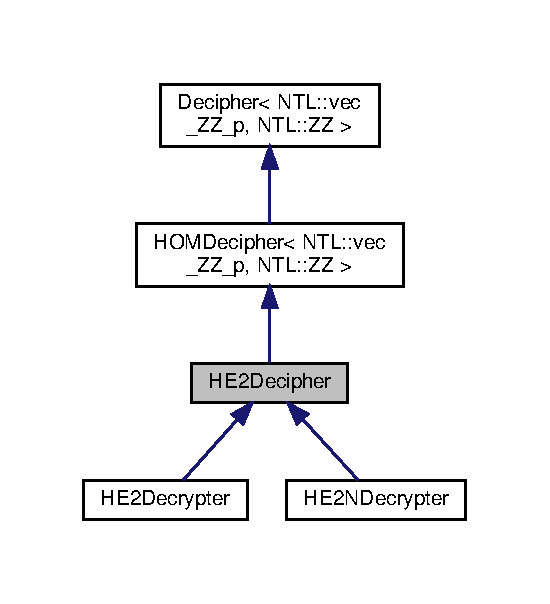
\includegraphics[width=264pt]{classHE2Decipher__inherit__graph}
\end{center}
\end{figure}


Collaboration diagram for H\+E2\+Decipher\+:\nopagebreak
\begin{figure}[H]
\begin{center}
\leavevmode
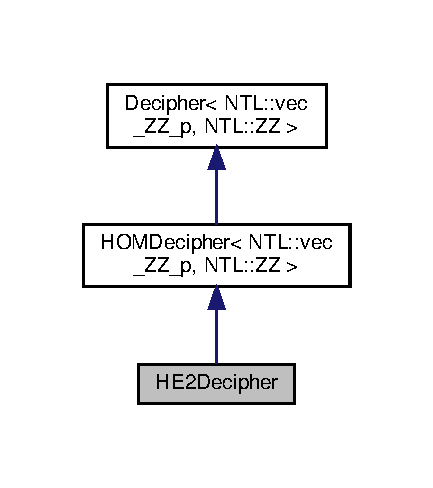
\includegraphics[width=208pt]{classHE2Decipher__coll__graph}
\end{center}
\end{figure}
\subsection*{Public Member Functions}
\begin{DoxyCompactItemize}
\item 
N\+T\+L\+::\+ZZ \hyperlink{classHE2Decipher_ac2b41a7a93daf683ab998f77cd59519c}{decrypt\+From\+String} (std\+::string \&str)
\item 
\hyperlink{classHE2Decipher_a80958b0ebcd436c8b580cb91a087bb38}{H\+E2\+Decipher} ()
\item 
virtual \hyperlink{classHE2Decipher_a6f9d97ecc078e22b051fbf59b12fff89}{$\sim$\+H\+E2\+Decipher} ()
\end{DoxyCompactItemize}
\subsection*{Protected Attributes}
\begin{DoxyCompactItemize}
\item 
N\+T\+L\+::\+ZZ \hyperlink{classHE2Decipher_ae77640302cf735f4b9b3a74d9da87563}{modulus}
\item 
N\+T\+L\+::vec\+\_\+\+Z\+Z\+\_\+p $\ast$ \hyperlink{classHE2Decipher_a08f53cc4849910945d4ba7f4f16e93a2}{gamma}
\end{DoxyCompactItemize}


\subsection{Constructor \& Destructor Documentation}
\mbox{\Hypertarget{classHE2Decipher_a80958b0ebcd436c8b580cb91a087bb38}\label{classHE2Decipher_a80958b0ebcd436c8b580cb91a087bb38}} 
\index{H\+E2\+Decipher@{H\+E2\+Decipher}!H\+E2\+Decipher@{H\+E2\+Decipher}}
\index{H\+E2\+Decipher@{H\+E2\+Decipher}!H\+E2\+Decipher@{H\+E2\+Decipher}}
\subsubsection{\texorpdfstring{H\+E2\+Decipher()}{HE2Decipher()}}
{\footnotesize\ttfamily H\+E2\+Decipher\+::\+H\+E2\+Decipher (\begin{DoxyParamCaption}{ }\end{DoxyParamCaption})}

\mbox{\Hypertarget{classHE2Decipher_a6f9d97ecc078e22b051fbf59b12fff89}\label{classHE2Decipher_a6f9d97ecc078e22b051fbf59b12fff89}} 
\index{H\+E2\+Decipher@{H\+E2\+Decipher}!````~H\+E2\+Decipher@{$\sim$\+H\+E2\+Decipher}}
\index{````~H\+E2\+Decipher@{$\sim$\+H\+E2\+Decipher}!H\+E2\+Decipher@{H\+E2\+Decipher}}
\subsubsection{\texorpdfstring{$\sim$\+H\+E2\+Decipher()}{~HE2Decipher()}}
{\footnotesize\ttfamily H\+E2\+Decipher\+::$\sim$\+H\+E2\+Decipher (\begin{DoxyParamCaption}{ }\end{DoxyParamCaption})\hspace{0.3cm}{\ttfamily [virtual]}}



\subsection{Member Function Documentation}
\mbox{\Hypertarget{classHE2Decipher_ac2b41a7a93daf683ab998f77cd59519c}\label{classHE2Decipher_ac2b41a7a93daf683ab998f77cd59519c}} 
\index{H\+E2\+Decipher@{H\+E2\+Decipher}!decrypt\+From\+String@{decrypt\+From\+String}}
\index{decrypt\+From\+String@{decrypt\+From\+String}!H\+E2\+Decipher@{H\+E2\+Decipher}}
\subsubsection{\texorpdfstring{decrypt\+From\+String()}{decryptFromString()}}
{\footnotesize\ttfamily N\+T\+L\+::\+ZZ H\+E2\+Decipher\+::decrypt\+From\+String (\begin{DoxyParamCaption}\item[{std\+::string \&}]{str }\end{DoxyParamCaption})}

Auxiliary method to decrypt a string respresentation of the 2-\/vector ciphertext 
\begin{DoxyParams}{Parameters}
{\em str} & A string respresentation of the ciphertext \\
\hline
\end{DoxyParams}
\begin{DoxyReturn}{Returns}
A multiprecision integer 
\end{DoxyReturn}


\subsection{Member Data Documentation}
\mbox{\Hypertarget{classHE2Decipher_a08f53cc4849910945d4ba7f4f16e93a2}\label{classHE2Decipher_a08f53cc4849910945d4ba7f4f16e93a2}} 
\index{H\+E2\+Decipher@{H\+E2\+Decipher}!gamma@{gamma}}
\index{gamma@{gamma}!H\+E2\+Decipher@{H\+E2\+Decipher}}
\subsubsection{\texorpdfstring{gamma}{gamma}}
{\footnotesize\ttfamily N\+T\+L\+::vec\+\_\+\+Z\+Z\+\_\+p$\ast$ H\+E2\+Decipher\+::gamma\hspace{0.3cm}{\ttfamily [protected]}}

The decryption vector. This is a pointer to avoid gamma being initialised mod zero \mbox{\Hypertarget{classHE2Decipher_ae77640302cf735f4b9b3a74d9da87563}\label{classHE2Decipher_ae77640302cf735f4b9b3a74d9da87563}} 
\index{H\+E2\+Decipher@{H\+E2\+Decipher}!modulus@{modulus}}
\index{modulus@{modulus}!H\+E2\+Decipher@{H\+E2\+Decipher}}
\subsubsection{\texorpdfstring{modulus}{modulus}}
{\footnotesize\ttfamily N\+T\+L\+::\+ZZ H\+E2\+Decipher\+::modulus\hspace{0.3cm}{\ttfamily [protected]}}

The public modulus for modular arithmetic. 

The documentation for this class was generated from the following files\+:\begin{DoxyCompactItemize}
\item 
include/\hyperlink{HE2Decipher_8h}{H\+E2\+Decipher.\+h}\item 
src/\hyperlink{HE2Decipher_8cpp}{H\+E2\+Decipher.\+cpp}\end{DoxyCompactItemize}

\hypertarget{classHE2Decrypter}{}\section{H\+E2\+Decrypter Class Reference}
\label{classHE2Decrypter}\index{H\+E2\+Decrypter@{H\+E2\+Decrypter}}


{\ttfamily \#include $<$H\+E2\+Decrypter.\+h$>$}



Inheritance diagram for H\+E2\+Decrypter\+:
\nopagebreak
\begin{figure}[H]
\begin{center}
\leavevmode
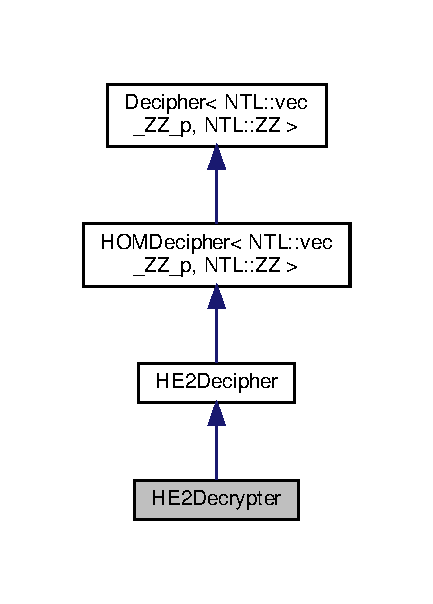
\includegraphics[width=208pt]{classHE2Decrypter__inherit__graph}
\end{center}
\end{figure}


Collaboration diagram for H\+E2\+Decrypter\+:
\nopagebreak
\begin{figure}[H]
\begin{center}
\leavevmode
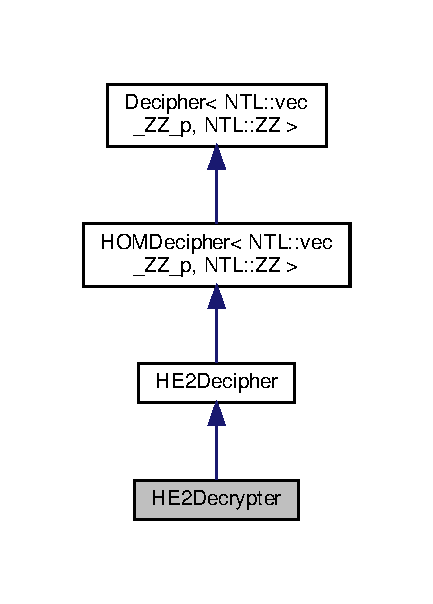
\includegraphics[width=208pt]{classHE2Decrypter__coll__graph}
\end{center}
\end{figure}
\subsection*{Public Member Functions}
\begin{DoxyCompactItemize}
\item 
void \hyperlink{classHE2Decrypter_a9cf1a6eae2667f6e891237589c4eeda0}{read\+Secrets\+From\+J\+S\+ON} (std\+::string \&json) override
\item 
N\+T\+L\+::\+ZZ \hyperlink{classHE2Decrypter_a766f96cb2277fd3e4af59ca44a32d519}{decrypt} (N\+T\+L\+::vec\+\_\+\+Z\+Z\+\_\+p \&ciphertext) override
\item 
virtual \hyperlink{classHE2Decrypter_a123b17b00516da42e87d7fa7d7911613}{$\sim$\+H\+E2\+Decrypter} ()
\item 
\hyperlink{classHE2Decrypter_a9ccbcb4de6bae54641e8777f9288d3f9}{H\+E2\+Decrypter} ()
\end{DoxyCompactItemize}
\subsection*{Additional Inherited Members}


\subsection{Constructor \& Destructor Documentation}
\mbox{\Hypertarget{classHE2Decrypter_a123b17b00516da42e87d7fa7d7911613}\label{classHE2Decrypter_a123b17b00516da42e87d7fa7d7911613}} 
\index{H\+E2\+Decrypter@{H\+E2\+Decrypter}!````~H\+E2\+Decrypter@{$\sim$\+H\+E2\+Decrypter}}
\index{````~H\+E2\+Decrypter@{$\sim$\+H\+E2\+Decrypter}!H\+E2\+Decrypter@{H\+E2\+Decrypter}}
\subsubsection{\texorpdfstring{$\sim$\+H\+E2\+Decrypter()}{~HE2Decrypter()}}
{\footnotesize\ttfamily H\+E2\+Decrypter\+::$\sim$\+H\+E2\+Decrypter (\begin{DoxyParamCaption}{ }\end{DoxyParamCaption})\hspace{0.3cm}{\ttfamily [virtual]}}

\mbox{\Hypertarget{classHE2Decrypter_a9ccbcb4de6bae54641e8777f9288d3f9}\label{classHE2Decrypter_a9ccbcb4de6bae54641e8777f9288d3f9}} 
\index{H\+E2\+Decrypter@{H\+E2\+Decrypter}!H\+E2\+Decrypter@{H\+E2\+Decrypter}}
\index{H\+E2\+Decrypter@{H\+E2\+Decrypter}!H\+E2\+Decrypter@{H\+E2\+Decrypter}}
\subsubsection{\texorpdfstring{H\+E2\+Decrypter()}{HE2Decrypter()}}
{\footnotesize\ttfamily H\+E2\+Decrypter\+::\+H\+E2\+Decrypter (\begin{DoxyParamCaption}{ }\end{DoxyParamCaption})}



\subsection{Member Function Documentation}
\mbox{\Hypertarget{classHE2Decrypter_a766f96cb2277fd3e4af59ca44a32d519}\label{classHE2Decrypter_a766f96cb2277fd3e4af59ca44a32d519}} 
\index{H\+E2\+Decrypter@{H\+E2\+Decrypter}!decrypt@{decrypt}}
\index{decrypt@{decrypt}!H\+E2\+Decrypter@{H\+E2\+Decrypter}}
\subsubsection{\texorpdfstring{decrypt()}{decrypt()}}
{\footnotesize\ttfamily N\+T\+L\+::\+ZZ H\+E2\+Decrypter\+::decrypt (\begin{DoxyParamCaption}\item[{N\+T\+L\+::vec\+\_\+\+Z\+Z\+\_\+p \&}]{ciphertext }\end{DoxyParamCaption})\hspace{0.3cm}{\ttfamily [override]}, {\ttfamily [virtual]}}



Implements \hyperlink{classDecipher_ac6b8c369eda2d7e17fa90cb594cf41b6}{Decipher$<$ N\+T\+L\+::vec\+\_\+\+Z\+Z\+\_\+p, N\+T\+L\+::\+Z\+Z $>$}.

\mbox{\Hypertarget{classHE2Decrypter_a9cf1a6eae2667f6e891237589c4eeda0}\label{classHE2Decrypter_a9cf1a6eae2667f6e891237589c4eeda0}} 
\index{H\+E2\+Decrypter@{H\+E2\+Decrypter}!read\+Secrets\+From\+J\+S\+ON@{read\+Secrets\+From\+J\+S\+ON}}
\index{read\+Secrets\+From\+J\+S\+ON@{read\+Secrets\+From\+J\+S\+ON}!H\+E2\+Decrypter@{H\+E2\+Decrypter}}
\subsubsection{\texorpdfstring{read\+Secrets\+From\+J\+S\+O\+N()}{readSecretsFromJSON()}}
{\footnotesize\ttfamily void H\+E2\+Decrypter\+::read\+Secrets\+From\+J\+S\+ON (\begin{DoxyParamCaption}\item[{std\+::string \&}]{json }\end{DoxyParamCaption})\hspace{0.3cm}{\ttfamily [override]}, {\ttfamily [virtual]}}



Implements \hyperlink{classDecipher_a39aea002012130201e12a8fa7d84dda5}{Decipher$<$ N\+T\+L\+::vec\+\_\+\+Z\+Z\+\_\+p, N\+T\+L\+::\+Z\+Z $>$}.



The documentation for this class was generated from the following files\+:\begin{DoxyCompactItemize}
\item 
include/\hyperlink{HE2Decrypter_8h}{H\+E2\+Decrypter.\+h}\item 
src/\hyperlink{HE2Decrypter_8cpp}{H\+E2\+Decrypter.\+cpp}\end{DoxyCompactItemize}

\hypertarget{classHE2Encipher}{}\section{H\+E2\+Encipher Class Reference}
\label{classHE2Encipher}\index{H\+E2\+Encipher@{H\+E2\+Encipher}}


{\ttfamily \#include $<$H\+E2\+Encipher.\+h$>$}



Inheritance diagram for H\+E2\+Encipher\+:\nopagebreak
\begin{figure}[H]
\begin{center}
\leavevmode
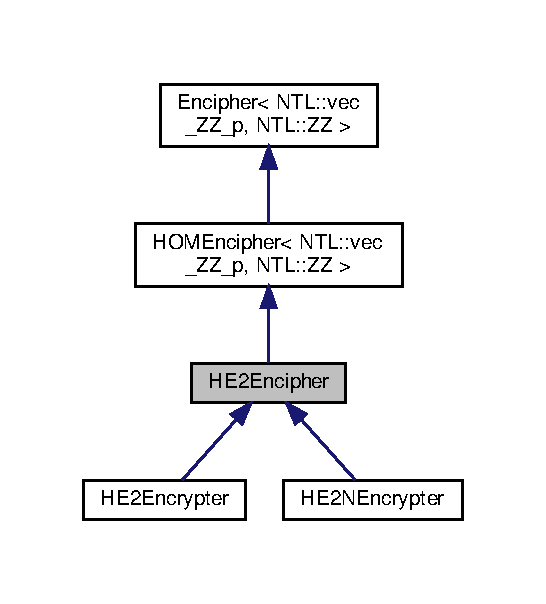
\includegraphics[width=262pt]{classHE2Encipher__inherit__graph}
\end{center}
\end{figure}


Collaboration diagram for H\+E2\+Encipher\+:\nopagebreak
\begin{figure}[H]
\begin{center}
\leavevmode
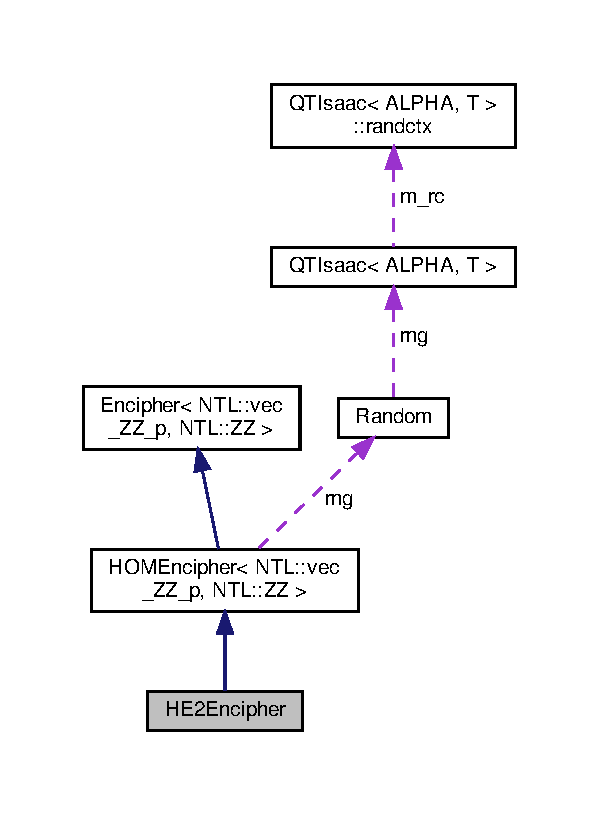
\includegraphics[width=288pt]{classHE2Encipher__coll__graph}
\end{center}
\end{figure}
\subsection*{Public Member Functions}
\begin{DoxyCompactItemize}
\item 
std\+::string \hyperlink{classHE2Encipher_a802a75d83bb833bf458a1e89792026bc}{write\+Parameters\+To\+J\+S\+ON} () override
\item 
virtual std\+::string \hyperlink{classHE2Encipher_a3546d0dfa3e656ec6fcde1c0a4678460}{encrypt\+To\+String} (int16\+\_\+t plaintext)
\item 
virtual std\+::string \hyperlink{classHE2Encipher_a10d552ea918c1c0a67f226745fed3ef6}{encrypt\+To\+String} (int32\+\_\+t plaintext)
\item 
virtual std\+::string \hyperlink{classHE2Encipher_a3c4dfca45e9f65955e64a328910b1339}{encrypt\+To\+String} (int64\+\_\+t plaintext)
\item 
virtual std\+::string \hyperlink{classHE2Encipher_a2b0d3c50f377d3cabe1a102f55ae2b48}{encrypt\+To\+String} (N\+T\+L\+::\+ZZ \&plaintext)
\item 
\hyperlink{classHE2Encipher_ab639560a28321b94af1ae72b7d375f58}{H\+E2\+Encipher} ()
\item 
virtual \hyperlink{classHE2Encipher_aa62b5f97090f8b14eeeff436664ef8e6}{$\sim$\+H\+E2\+Encipher} ()
\end{DoxyCompactItemize}
\subsection*{Static Public Attributes}
\begin{DoxyCompactItemize}
\item 
static N\+T\+L\+::\+ZZ \hyperlink{classHE2Encipher_a85145ccd52161ab492eca360daad9b00}{O\+NE} = N\+T\+L\+::\+ZZ(1)
\item 
static N\+T\+L\+::vec\+\_\+\+Z\+Z\+\_\+p \hyperlink{classHE2Encipher_a4099b9dff30fbe3fa5a36d7f5a8a2073}{O\+N\+E\+\_\+\+V\+E\+C\+T\+OR}
\end{DoxyCompactItemize}
\subsection*{Protected Member Functions}
\begin{DoxyCompactItemize}
\item 
void \hyperlink{classHE2Encipher_a13305651228f50d55e6ee905032e01af}{generate\+Parameters} (int lambda, int eta)
\end{DoxyCompactItemize}
\subsection*{Protected Attributes}
\begin{DoxyCompactItemize}
\item 
N\+T\+L\+::vec\+\_\+\+Z\+Z\+\_\+p $\ast$ \hyperlink{classHE2Encipher_a84192e155c19195867671fa085f9c73c}{a}
\item 
N\+T\+L\+::mat\+\_\+\+Z\+Z\+\_\+p $\ast$ \hyperlink{classHE2Encipher_af01e9f2e19df354cecde3f7ea66524a0}{R}
\item 
N\+T\+L\+::vec\+\_\+\+Z\+Z\+\_\+p $\ast$ \hyperlink{classHE2Encipher_acb629492d1edb07e4ac6d2dca60c582a}{gamma}
\item 
N\+T\+L\+::\+Z\+Z\+\_\+p $\ast$ \hyperlink{classHE2Encipher_a0fc7c51d125b4b638b59dfe5bd99976c}{pmod}
\end{DoxyCompactItemize}


\subsection{Constructor \& Destructor Documentation}
\mbox{\Hypertarget{classHE2Encipher_ab639560a28321b94af1ae72b7d375f58}\label{classHE2Encipher_ab639560a28321b94af1ae72b7d375f58}} 
\index{H\+E2\+Encipher@{H\+E2\+Encipher}!H\+E2\+Encipher@{H\+E2\+Encipher}}
\index{H\+E2\+Encipher@{H\+E2\+Encipher}!H\+E2\+Encipher@{H\+E2\+Encipher}}
\subsubsection{\texorpdfstring{H\+E2\+Encipher()}{HE2Encipher()}}
{\footnotesize\ttfamily H\+E2\+Encipher\+::\+H\+E2\+Encipher (\begin{DoxyParamCaption}{ }\end{DoxyParamCaption})}

\mbox{\Hypertarget{classHE2Encipher_aa62b5f97090f8b14eeeff436664ef8e6}\label{classHE2Encipher_aa62b5f97090f8b14eeeff436664ef8e6}} 
\index{H\+E2\+Encipher@{H\+E2\+Encipher}!````~H\+E2\+Encipher@{$\sim$\+H\+E2\+Encipher}}
\index{````~H\+E2\+Encipher@{$\sim$\+H\+E2\+Encipher}!H\+E2\+Encipher@{H\+E2\+Encipher}}
\subsubsection{\texorpdfstring{$\sim$\+H\+E2\+Encipher()}{~HE2Encipher()}}
{\footnotesize\ttfamily H\+E2\+Encipher\+::$\sim$\+H\+E2\+Encipher (\begin{DoxyParamCaption}{ }\end{DoxyParamCaption})\hspace{0.3cm}{\ttfamily [virtual]}}



\subsection{Member Function Documentation}
\mbox{\Hypertarget{classHE2Encipher_a3546d0dfa3e656ec6fcde1c0a4678460}\label{classHE2Encipher_a3546d0dfa3e656ec6fcde1c0a4678460}} 
\index{H\+E2\+Encipher@{H\+E2\+Encipher}!encrypt\+To\+String@{encrypt\+To\+String}}
\index{encrypt\+To\+String@{encrypt\+To\+String}!H\+E2\+Encipher@{H\+E2\+Encipher}}
\subsubsection{\texorpdfstring{encrypt\+To\+String()}{encryptToString()}\hspace{0.1cm}{\footnotesize\ttfamily [1/4]}}
{\footnotesize\ttfamily std\+::string H\+E2\+Encipher\+::encrypt\+To\+String (\begin{DoxyParamCaption}\item[{int16\+\_\+t}]{plaintext }\end{DoxyParamCaption})\hspace{0.3cm}{\ttfamily [virtual]}}

Convenience method to encrypt a 16-\/bit integer to a string representation of the ciphertext 
\begin{DoxyParams}{Parameters}
{\em plaintext} & A 16-\/bit integer \\
\hline
\end{DoxyParams}
\begin{DoxyReturn}{Returns}
A string representation of the ciphertext 
\end{DoxyReturn}
\mbox{\Hypertarget{classHE2Encipher_a10d552ea918c1c0a67f226745fed3ef6}\label{classHE2Encipher_a10d552ea918c1c0a67f226745fed3ef6}} 
\index{H\+E2\+Encipher@{H\+E2\+Encipher}!encrypt\+To\+String@{encrypt\+To\+String}}
\index{encrypt\+To\+String@{encrypt\+To\+String}!H\+E2\+Encipher@{H\+E2\+Encipher}}
\subsubsection{\texorpdfstring{encrypt\+To\+String()}{encryptToString()}\hspace{0.1cm}{\footnotesize\ttfamily [2/4]}}
{\footnotesize\ttfamily std\+::string H\+E2\+Encipher\+::encrypt\+To\+String (\begin{DoxyParamCaption}\item[{int32\+\_\+t}]{plaintext }\end{DoxyParamCaption})\hspace{0.3cm}{\ttfamily [virtual]}}

Convenience method to encrypt a 32-\/bit integer to a string representation of the ciphertext 
\begin{DoxyParams}{Parameters}
{\em plaintext} & A 32-\/bit integer \\
\hline
\end{DoxyParams}
\begin{DoxyReturn}{Returns}
A string representation of the ciphertext 
\end{DoxyReturn}
\mbox{\Hypertarget{classHE2Encipher_a3c4dfca45e9f65955e64a328910b1339}\label{classHE2Encipher_a3c4dfca45e9f65955e64a328910b1339}} 
\index{H\+E2\+Encipher@{H\+E2\+Encipher}!encrypt\+To\+String@{encrypt\+To\+String}}
\index{encrypt\+To\+String@{encrypt\+To\+String}!H\+E2\+Encipher@{H\+E2\+Encipher}}
\subsubsection{\texorpdfstring{encrypt\+To\+String()}{encryptToString()}\hspace{0.1cm}{\footnotesize\ttfamily [3/4]}}
{\footnotesize\ttfamily std\+::string H\+E2\+Encipher\+::encrypt\+To\+String (\begin{DoxyParamCaption}\item[{int64\+\_\+t}]{plaintext }\end{DoxyParamCaption})\hspace{0.3cm}{\ttfamily [virtual]}}

Convenience method to encrypt a 64-\/bit integer to a string representation of the ciphertext 
\begin{DoxyParams}{Parameters}
{\em plaintext} & A 64-\/bit integer \\
\hline
\end{DoxyParams}
\begin{DoxyReturn}{Returns}
A string representation of the ciphertext 
\end{DoxyReturn}
\mbox{\Hypertarget{classHE2Encipher_a2b0d3c50f377d3cabe1a102f55ae2b48}\label{classHE2Encipher_a2b0d3c50f377d3cabe1a102f55ae2b48}} 
\index{H\+E2\+Encipher@{H\+E2\+Encipher}!encrypt\+To\+String@{encrypt\+To\+String}}
\index{encrypt\+To\+String@{encrypt\+To\+String}!H\+E2\+Encipher@{H\+E2\+Encipher}}
\subsubsection{\texorpdfstring{encrypt\+To\+String()}{encryptToString()}\hspace{0.1cm}{\footnotesize\ttfamily [4/4]}}
{\footnotesize\ttfamily std\+::string H\+E2\+Encipher\+::encrypt\+To\+String (\begin{DoxyParamCaption}\item[{N\+T\+L\+::\+ZZ \&}]{plaintext }\end{DoxyParamCaption})\hspace{0.3cm}{\ttfamily [virtual]}}

Convenience method to encrypt to a string representation of the ciphertext 
\begin{DoxyParams}{Parameters}
{\em plaintext} & A multiprecision integer \\
\hline
\end{DoxyParams}
\begin{DoxyReturn}{Returns}
A string representation of the ciphertext 
\end{DoxyReturn}
\mbox{\Hypertarget{classHE2Encipher_a13305651228f50d55e6ee905032e01af}\label{classHE2Encipher_a13305651228f50d55e6ee905032e01af}} 
\index{H\+E2\+Encipher@{H\+E2\+Encipher}!generate\+Parameters@{generate\+Parameters}}
\index{generate\+Parameters@{generate\+Parameters}!H\+E2\+Encipher@{H\+E2\+Encipher}}
\subsubsection{\texorpdfstring{generate\+Parameters()}{generateParameters()}}
{\footnotesize\ttfamily void H\+E2\+Encipher\+::generate\+Parameters (\begin{DoxyParamCaption}\item[{int}]{lambda,  }\item[{int}]{eta }\end{DoxyParamCaption})\hspace{0.3cm}{\ttfamily [protected]}}

Generate the cipher parameters common to the H\+E2 and H\+E2N ciphers. This method generates {\ttfamily a}, {\ttfamily gamma}, and {\ttfamily R}. 
\begin{DoxyParams}{Parameters}
{\em lambda} & The bit length of {\ttfamily p} \\
\hline
{\em eta} & The bit length of {\ttfamily q} where the modulus is {\ttfamily pq} \\
\hline
\end{DoxyParams}
\mbox{\Hypertarget{classHE2Encipher_a802a75d83bb833bf458a1e89792026bc}\label{classHE2Encipher_a802a75d83bb833bf458a1e89792026bc}} 
\index{H\+E2\+Encipher@{H\+E2\+Encipher}!write\+Parameters\+To\+J\+S\+ON@{write\+Parameters\+To\+J\+S\+ON}}
\index{write\+Parameters\+To\+J\+S\+ON@{write\+Parameters\+To\+J\+S\+ON}!H\+E2\+Encipher@{H\+E2\+Encipher}}
\subsubsection{\texorpdfstring{write\+Parameters\+To\+J\+S\+O\+N()}{writeParametersToJSON()}}
{\footnotesize\ttfamily std\+::string H\+E2\+Encipher\+::write\+Parameters\+To\+J\+S\+ON (\begin{DoxyParamCaption}{ }\end{DoxyParamCaption})\hspace{0.3cm}{\ttfamily [override]}, {\ttfamily [virtual]}}

Write the public cipher parameters to a J\+S\+ON string \begin{DoxyReturn}{Returns}
J\+S\+ON string 
\end{DoxyReturn}


Implements \hyperlink{classHOMEncipher_abf176e3fb85de6f0f6a2c96563397d39}{H\+O\+M\+Encipher$<$ N\+T\+L\+::vec\+\_\+\+Z\+Z\+\_\+p, N\+T\+L\+::\+Z\+Z $>$}.



\subsection{Member Data Documentation}
\mbox{\Hypertarget{classHE2Encipher_a84192e155c19195867671fa085f9c73c}\label{classHE2Encipher_a84192e155c19195867671fa085f9c73c}} 
\index{H\+E2\+Encipher@{H\+E2\+Encipher}!a@{a}}
\index{a@{a}!H\+E2\+Encipher@{H\+E2\+Encipher}}
\subsubsection{\texorpdfstring{a}{a}}
{\footnotesize\ttfamily N\+T\+L\+::vec\+\_\+\+Z\+Z\+\_\+p$\ast$ H\+E2\+Encipher\+::a\hspace{0.3cm}{\ttfamily [protected]}}

The secret vector of the cipher. This is a pointer to avoid a being initialised mod zero. \mbox{\Hypertarget{classHE2Encipher_acb629492d1edb07e4ac6d2dca60c582a}\label{classHE2Encipher_acb629492d1edb07e4ac6d2dca60c582a}} 
\index{H\+E2\+Encipher@{H\+E2\+Encipher}!gamma@{gamma}}
\index{gamma@{gamma}!H\+E2\+Encipher@{H\+E2\+Encipher}}
\subsubsection{\texorpdfstring{gamma}{gamma}}
{\footnotesize\ttfamily N\+T\+L\+::vec\+\_\+\+Z\+Z\+\_\+p$\ast$ H\+E2\+Encipher\+::gamma\hspace{0.3cm}{\ttfamily [protected]}}

The secret decryption vector. This is a pointer to avoid gamma being initialised mod zero. \mbox{\Hypertarget{classHE2Encipher_a85145ccd52161ab492eca360daad9b00}\label{classHE2Encipher_a85145ccd52161ab492eca360daad9b00}} 
\index{H\+E2\+Encipher@{H\+E2\+Encipher}!O\+NE@{O\+NE}}
\index{O\+NE@{O\+NE}!H\+E2\+Encipher@{H\+E2\+Encipher}}
\subsubsection{\texorpdfstring{O\+NE}{ONE}}
{\footnotesize\ttfamily N\+T\+L\+::\+ZZ H\+E2\+Encipher\+::\+O\+NE = N\+T\+L\+::\+ZZ(1)\hspace{0.3cm}{\ttfamily [static]}}

One as a multiprecision integer \mbox{\Hypertarget{classHE2Encipher_a4099b9dff30fbe3fa5a36d7f5a8a2073}\label{classHE2Encipher_a4099b9dff30fbe3fa5a36d7f5a8a2073}} 
\index{H\+E2\+Encipher@{H\+E2\+Encipher}!O\+N\+E\+\_\+\+V\+E\+C\+T\+OR@{O\+N\+E\+\_\+\+V\+E\+C\+T\+OR}}
\index{O\+N\+E\+\_\+\+V\+E\+C\+T\+OR@{O\+N\+E\+\_\+\+V\+E\+C\+T\+OR}!H\+E2\+Encipher@{H\+E2\+Encipher}}
\subsubsection{\texorpdfstring{O\+N\+E\+\_\+\+V\+E\+C\+T\+OR}{ONE\_VECTOR}}
{\footnotesize\ttfamily N\+T\+L\+::vec\+\_\+\+Z\+Z\+\_\+p H\+E2\+Encipher\+::\+O\+N\+E\+\_\+\+V\+E\+C\+T\+OR\hspace{0.3cm}{\ttfamily [static]}}

The vector \mbox{[}1 1\mbox{]}$^\wedge$T \mbox{\Hypertarget{classHE2Encipher_a0fc7c51d125b4b638b59dfe5bd99976c}\label{classHE2Encipher_a0fc7c51d125b4b638b59dfe5bd99976c}} 
\index{H\+E2\+Encipher@{H\+E2\+Encipher}!pmod@{pmod}}
\index{pmod@{pmod}!H\+E2\+Encipher@{H\+E2\+Encipher}}
\subsubsection{\texorpdfstring{pmod}{pmod}}
{\footnotesize\ttfamily N\+T\+L\+::\+Z\+Z\+\_\+p$\ast$ H\+E2\+Encipher\+::pmod\hspace{0.3cm}{\ttfamily [protected]}}

The secret key as a modulo integer. This is for convenience to avoid having to convert multiple times. This is a pointer to avoid pmod being initialised mod zero. \mbox{\Hypertarget{classHE2Encipher_af01e9f2e19df354cecde3f7ea66524a0}\label{classHE2Encipher_af01e9f2e19df354cecde3f7ea66524a0}} 
\index{H\+E2\+Encipher@{H\+E2\+Encipher}!R@{R}}
\index{R@{R}!H\+E2\+Encipher@{H\+E2\+Encipher}}
\subsubsection{\texorpdfstring{R}{R}}
{\footnotesize\ttfamily N\+T\+L\+::mat\+\_\+\+Z\+Z\+\_\+p$\ast$ H\+E2\+Encipher\+::R\hspace{0.3cm}{\ttfamily [protected]}}

The public re-\/encryption matrix. This is a pointer to avoid R being initialised mod zero. 

The documentation for this class was generated from the following files\+:\begin{DoxyCompactItemize}
\item 
include/\hyperlink{HE2Encipher_8h}{H\+E2\+Encipher.\+h}\item 
src/\hyperlink{HE2Encipher_8cpp}{H\+E2\+Encipher.\+cpp}\end{DoxyCompactItemize}

\hypertarget{classHE2Encrypter}{}\section{H\+E2\+Encrypter Class Reference}
\label{classHE2Encrypter}\index{H\+E2\+Encrypter@{H\+E2\+Encrypter}}


{\ttfamily \#include $<$H\+E2\+Encrypter.\+h$>$}



Inheritance diagram for H\+E2\+Encrypter\+:\nopagebreak
\begin{figure}[H]
\begin{center}
\leavevmode
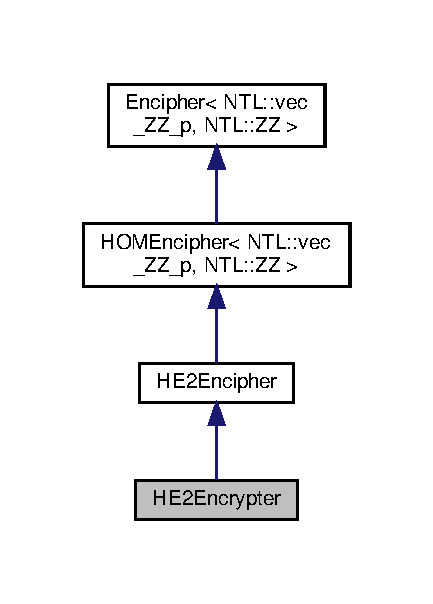
\includegraphics[width=208pt]{classHE2Encrypter__inherit__graph}
\end{center}
\end{figure}


Collaboration diagram for H\+E2\+Encrypter\+:\nopagebreak
\begin{figure}[H]
\begin{center}
\leavevmode
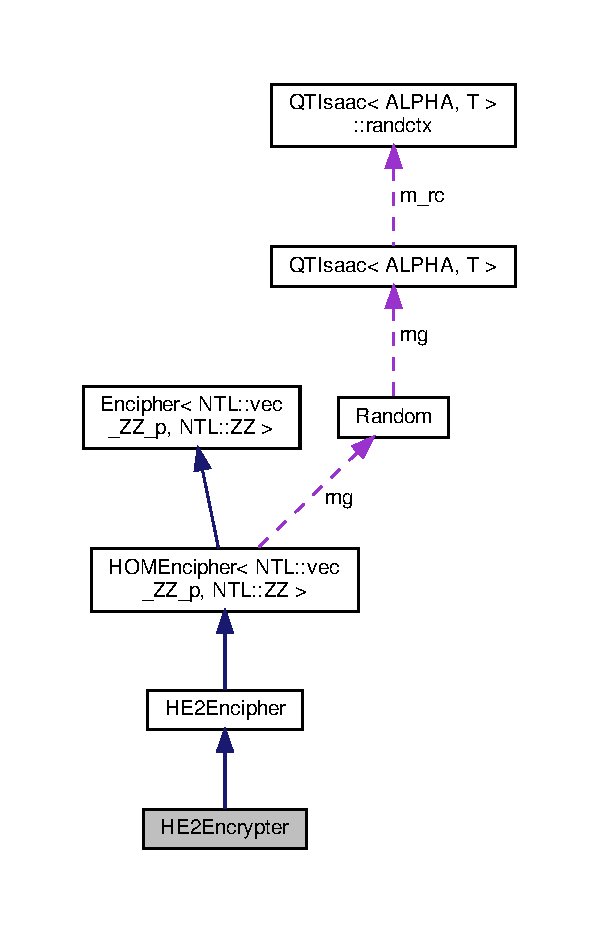
\includegraphics[width=288pt]{classHE2Encrypter__coll__graph}
\end{center}
\end{figure}
\subsection*{Public Member Functions}
\begin{DoxyCompactItemize}
\item 
std\+::string \hyperlink{classHE2Encrypter_a8cdf863bfbe046b4e57322adf5addddb}{write\+Secrets\+To\+J\+S\+ON} () override
\item 
N\+T\+L\+::vec\+\_\+\+Z\+Z\+\_\+p \hyperlink{classHE2Encrypter_a57e4bdacbab9b11467f26deab921d134}{encrypt} (N\+T\+L\+::\+ZZ \&plaintext) override
\item 
\hyperlink{classHE2Encrypter_afa15786431e27f582fb4b62282407ed4}{H\+E2\+Encrypter} (int lambda, int eta)
\item 
\hyperlink{classHE2Encrypter_a38f4e27834ca8d2f2169dd8618e66650}{H\+E2\+Encrypter} (int n, int d, int rho)
\item 
virtual \hyperlink{classHE2Encrypter_a22a4b92894ca930ee234c219d7d2038e}{$\sim$\+H\+E2\+Encrypter} ()
\end{DoxyCompactItemize}
\subsection*{Additional Inherited Members}


\subsection{Constructor \& Destructor Documentation}
\mbox{\Hypertarget{classHE2Encrypter_afa15786431e27f582fb4b62282407ed4}\label{classHE2Encrypter_afa15786431e27f582fb4b62282407ed4}} 
\index{H\+E2\+Encrypter@{H\+E2\+Encrypter}!H\+E2\+Encrypter@{H\+E2\+Encrypter}}
\index{H\+E2\+Encrypter@{H\+E2\+Encrypter}!H\+E2\+Encrypter@{H\+E2\+Encrypter}}
\subsubsection{\texorpdfstring{H\+E2\+Encrypter()}{HE2Encrypter()}\hspace{0.1cm}{\footnotesize\ttfamily [1/2]}}
{\footnotesize\ttfamily H\+E2\+Encrypter\+::\+H\+E2\+Encrypter (\begin{DoxyParamCaption}\item[{int}]{lambda,  }\item[{int}]{eta }\end{DoxyParamCaption})}

Initialise cipher by generating cipher parameters such that {\ttfamily p} is a {\ttfamily lambda} bit prime and {\ttfamily q} is an {\ttfamily eta} bit prime. The public modulus for arithmetic operations on ciphertexts is {\ttfamily pq} 
\begin{DoxyParams}{Parameters}
{\em lambda} & Bit length of secret modulus {\ttfamily p} (security parameter) \\
\hline
{\em eta} & Bit length of secret prime {\ttfamily q}. \\
\hline
\end{DoxyParams}
\mbox{\Hypertarget{classHE2Encrypter_a38f4e27834ca8d2f2169dd8618e66650}\label{classHE2Encrypter_a38f4e27834ca8d2f2169dd8618e66650}} 
\index{H\+E2\+Encrypter@{H\+E2\+Encrypter}!H\+E2\+Encrypter@{H\+E2\+Encrypter}}
\index{H\+E2\+Encrypter@{H\+E2\+Encrypter}!H\+E2\+Encrypter@{H\+E2\+Encrypter}}
\subsubsection{\texorpdfstring{H\+E2\+Encrypter()}{HE2Encrypter()}\hspace{0.1cm}{\footnotesize\ttfamily [2/2]}}
{\footnotesize\ttfamily H\+E2\+Encrypter\+::\+H\+E2\+Encrypter (\begin{DoxyParamCaption}\item[{int}]{n,  }\item[{int}]{d,  }\item[{int}]{rho }\end{DoxyParamCaption})}

Initialise cipher by generating cipher parameters so that {\ttfamily p} is large enough to accommodate a degree {\ttfamily d} multivariate polynomial computed over {\ttfamily n} {\ttfamily rho\%-\/bit} integer inputs and {\ttfamily q} is large enough so that pq cannot be factored in polynomial time. 
\begin{DoxyParams}{Parameters}
{\em n} & total number of inputs \\
\hline
{\em d} & degree of polynomial to compute \\
\hline
{\em rho} & bit length of inputs, e.\+g for 32-\/bit integers {\ttfamily rho} = 32 \\
\hline
\end{DoxyParams}
\mbox{\Hypertarget{classHE2Encrypter_a22a4b92894ca930ee234c219d7d2038e}\label{classHE2Encrypter_a22a4b92894ca930ee234c219d7d2038e}} 
\index{H\+E2\+Encrypter@{H\+E2\+Encrypter}!````~H\+E2\+Encrypter@{$\sim$\+H\+E2\+Encrypter}}
\index{````~H\+E2\+Encrypter@{$\sim$\+H\+E2\+Encrypter}!H\+E2\+Encrypter@{H\+E2\+Encrypter}}
\subsubsection{\texorpdfstring{$\sim$\+H\+E2\+Encrypter()}{~HE2Encrypter()}}
{\footnotesize\ttfamily virtual H\+E2\+Encrypter\+::$\sim$\+H\+E2\+Encrypter (\begin{DoxyParamCaption}{ }\end{DoxyParamCaption})\hspace{0.3cm}{\ttfamily [inline]}, {\ttfamily [virtual]}}



\subsection{Member Function Documentation}
\mbox{\Hypertarget{classHE2Encrypter_a57e4bdacbab9b11467f26deab921d134}\label{classHE2Encrypter_a57e4bdacbab9b11467f26deab921d134}} 
\index{H\+E2\+Encrypter@{H\+E2\+Encrypter}!encrypt@{encrypt}}
\index{encrypt@{encrypt}!H\+E2\+Encrypter@{H\+E2\+Encrypter}}
\subsubsection{\texorpdfstring{encrypt()}{encrypt()}}
{\footnotesize\ttfamily N\+T\+L\+::vec\+\_\+\+Z\+Z\+\_\+p H\+E2\+Encrypter\+::encrypt (\begin{DoxyParamCaption}\item[{N\+T\+L\+::\+ZZ \&}]{plaintext }\end{DoxyParamCaption})\hspace{0.3cm}{\ttfamily [override]}, {\ttfamily [virtual]}}

Encrypt a plaintext 
\begin{DoxyParams}{Parameters}
{\em plaintext} & A plaintext value \\
\hline
\end{DoxyParams}
\begin{DoxyReturn}{Returns}
A ciphertext value 
\end{DoxyReturn}


Implements \hyperlink{classEncipher_aaf8138eb280608bfd03c6eb762ffc010}{Encipher$<$ N\+T\+L\+::vec\+\_\+\+Z\+Z\+\_\+p, N\+T\+L\+::\+Z\+Z $>$}.

\mbox{\Hypertarget{classHE2Encrypter_a8cdf863bfbe046b4e57322adf5addddb}\label{classHE2Encrypter_a8cdf863bfbe046b4e57322adf5addddb}} 
\index{H\+E2\+Encrypter@{H\+E2\+Encrypter}!write\+Secrets\+To\+J\+S\+ON@{write\+Secrets\+To\+J\+S\+ON}}
\index{write\+Secrets\+To\+J\+S\+ON@{write\+Secrets\+To\+J\+S\+ON}!H\+E2\+Encrypter@{H\+E2\+Encrypter}}
\subsubsection{\texorpdfstring{write\+Secrets\+To\+J\+S\+O\+N()}{writeSecretsToJSON()}}
{\footnotesize\ttfamily std\+::string H\+E2\+Encrypter\+::write\+Secrets\+To\+J\+S\+ON (\begin{DoxyParamCaption}{ }\end{DoxyParamCaption})\hspace{0.3cm}{\ttfamily [override]}, {\ttfamily [virtual]}}

Writes cipher secrets out to a J\+S\+ON string \begin{DoxyReturn}{Returns}
J\+S\+ON string 
\end{DoxyReturn}


Implements \hyperlink{classEncipher_a27d3efa1e364c1f0d7def65454c61b85}{Encipher$<$ N\+T\+L\+::vec\+\_\+\+Z\+Z\+\_\+p, N\+T\+L\+::\+Z\+Z $>$}.



The documentation for this class was generated from the following files\+:\begin{DoxyCompactItemize}
\item 
include/\hyperlink{HE2Encrypter_8h}{H\+E2\+Encrypter.\+h}\item 
src/\hyperlink{HE2Encrypter_8cpp}{H\+E2\+Encrypter.\+cpp}\end{DoxyCompactItemize}

\hypertarget{classHE2NDecrypter}{}\section{H\+E2\+N\+Decrypter Class Reference}
\label{classHE2NDecrypter}\index{H\+E2\+N\+Decrypter@{H\+E2\+N\+Decrypter}}


{\ttfamily \#include $<$H\+E2\+N\+Decrypter.\+h$>$}



Inheritance diagram for H\+E2\+N\+Decrypter\+:
\nopagebreak
\begin{figure}[H]
\begin{center}
\leavevmode
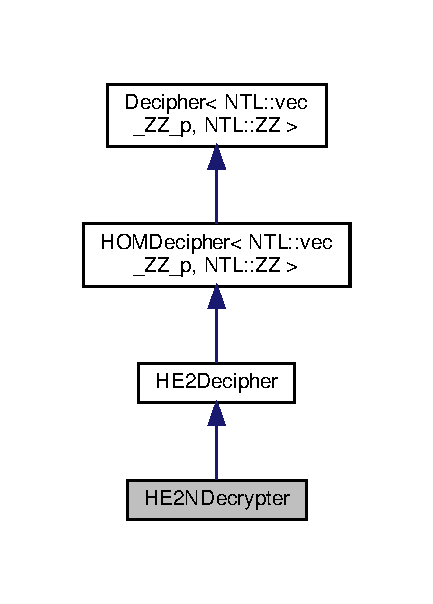
\includegraphics[width=208pt]{classHE2NDecrypter__inherit__graph}
\end{center}
\end{figure}


Collaboration diagram for H\+E2\+N\+Decrypter\+:
\nopagebreak
\begin{figure}[H]
\begin{center}
\leavevmode
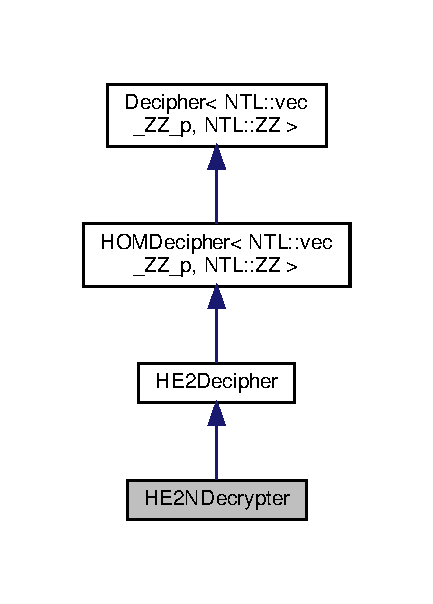
\includegraphics[width=208pt]{classHE2NDecrypter__coll__graph}
\end{center}
\end{figure}
\subsection*{Public Member Functions}
\begin{DoxyCompactItemize}
\item 
void \hyperlink{classHE2NDecrypter_a92b463d8e18d2f06d0680528edfd49c4}{read\+Secrets\+From\+J\+S\+ON} (std\+::string \&json) override
\item 
N\+T\+L\+::\+ZZ \hyperlink{classHE2NDecrypter_aa92e4ddf62a0f2c4199722983e28b0c9}{decrypt} (N\+T\+L\+::vec\+\_\+\+Z\+Z\+\_\+p \&ciphertext) override
\item 
\hyperlink{classHE2NDecrypter_a079e13cfaf35e9f4b32d4301960c6816}{H\+E2\+N\+Decrypter} ()
\item 
virtual \hyperlink{classHE2NDecrypter_a5e6c617b905b370d5186e7d4193fd5b8}{$\sim$\+H\+E2\+N\+Decrypter} ()
\end{DoxyCompactItemize}
\subsection*{Private Attributes}
\begin{DoxyCompactItemize}
\item 
N\+T\+L\+::\+ZZ \hyperlink{classHE2NDecrypter_ad3233fd048ef07f31e4f40ea941cce91}{kappa}
\end{DoxyCompactItemize}
\subsection*{Additional Inherited Members}


\subsection{Constructor \& Destructor Documentation}
\mbox{\Hypertarget{classHE2NDecrypter_a079e13cfaf35e9f4b32d4301960c6816}\label{classHE2NDecrypter_a079e13cfaf35e9f4b32d4301960c6816}} 
\index{H\+E2\+N\+Decrypter@{H\+E2\+N\+Decrypter}!H\+E2\+N\+Decrypter@{H\+E2\+N\+Decrypter}}
\index{H\+E2\+N\+Decrypter@{H\+E2\+N\+Decrypter}!H\+E2\+N\+Decrypter@{H\+E2\+N\+Decrypter}}
\subsubsection{\texorpdfstring{H\+E2\+N\+Decrypter()}{HE2NDecrypter()}}
{\footnotesize\ttfamily H\+E2\+N\+Decrypter\+::\+H\+E2\+N\+Decrypter (\begin{DoxyParamCaption}{ }\end{DoxyParamCaption})}

\mbox{\Hypertarget{classHE2NDecrypter_a5e6c617b905b370d5186e7d4193fd5b8}\label{classHE2NDecrypter_a5e6c617b905b370d5186e7d4193fd5b8}} 
\index{H\+E2\+N\+Decrypter@{H\+E2\+N\+Decrypter}!````~H\+E2\+N\+Decrypter@{$\sim$\+H\+E2\+N\+Decrypter}}
\index{````~H\+E2\+N\+Decrypter@{$\sim$\+H\+E2\+N\+Decrypter}!H\+E2\+N\+Decrypter@{H\+E2\+N\+Decrypter}}
\subsubsection{\texorpdfstring{$\sim$\+H\+E2\+N\+Decrypter()}{~HE2NDecrypter()}}
{\footnotesize\ttfamily H\+E2\+N\+Decrypter\+::$\sim$\+H\+E2\+N\+Decrypter (\begin{DoxyParamCaption}{ }\end{DoxyParamCaption})\hspace{0.3cm}{\ttfamily [virtual]}}



\subsection{Member Function Documentation}
\mbox{\Hypertarget{classHE2NDecrypter_aa92e4ddf62a0f2c4199722983e28b0c9}\label{classHE2NDecrypter_aa92e4ddf62a0f2c4199722983e28b0c9}} 
\index{H\+E2\+N\+Decrypter@{H\+E2\+N\+Decrypter}!decrypt@{decrypt}}
\index{decrypt@{decrypt}!H\+E2\+N\+Decrypter@{H\+E2\+N\+Decrypter}}
\subsubsection{\texorpdfstring{decrypt()}{decrypt()}}
{\footnotesize\ttfamily N\+T\+L\+::\+ZZ H\+E2\+N\+Decrypter\+::decrypt (\begin{DoxyParamCaption}\item[{N\+T\+L\+::vec\+\_\+\+Z\+Z\+\_\+p \&}]{ciphertext }\end{DoxyParamCaption})\hspace{0.3cm}{\ttfamily [override]}, {\ttfamily [virtual]}}



Implements \hyperlink{classDecipher_ac6b8c369eda2d7e17fa90cb594cf41b6}{Decipher$<$ N\+T\+L\+::vec\+\_\+\+Z\+Z\+\_\+p, N\+T\+L\+::\+Z\+Z $>$}.

\mbox{\Hypertarget{classHE2NDecrypter_a92b463d8e18d2f06d0680528edfd49c4}\label{classHE2NDecrypter_a92b463d8e18d2f06d0680528edfd49c4}} 
\index{H\+E2\+N\+Decrypter@{H\+E2\+N\+Decrypter}!read\+Secrets\+From\+J\+S\+ON@{read\+Secrets\+From\+J\+S\+ON}}
\index{read\+Secrets\+From\+J\+S\+ON@{read\+Secrets\+From\+J\+S\+ON}!H\+E2\+N\+Decrypter@{H\+E2\+N\+Decrypter}}
\subsubsection{\texorpdfstring{read\+Secrets\+From\+J\+S\+O\+N()}{readSecretsFromJSON()}}
{\footnotesize\ttfamily void H\+E2\+N\+Decrypter\+::read\+Secrets\+From\+J\+S\+ON (\begin{DoxyParamCaption}\item[{std\+::string \&}]{json }\end{DoxyParamCaption})\hspace{0.3cm}{\ttfamily [override]}, {\ttfamily [virtual]}}



Implements \hyperlink{classDecipher_a39aea002012130201e12a8fa7d84dda5}{Decipher$<$ N\+T\+L\+::vec\+\_\+\+Z\+Z\+\_\+p, N\+T\+L\+::\+Z\+Z $>$}.



\subsection{Member Data Documentation}
\mbox{\Hypertarget{classHE2NDecrypter_ad3233fd048ef07f31e4f40ea941cce91}\label{classHE2NDecrypter_ad3233fd048ef07f31e4f40ea941cce91}} 
\index{H\+E2\+N\+Decrypter@{H\+E2\+N\+Decrypter}!kappa@{kappa}}
\index{kappa@{kappa}!H\+E2\+N\+Decrypter@{H\+E2\+N\+Decrypter}}
\subsubsection{\texorpdfstring{kappa}{kappa}}
{\footnotesize\ttfamily N\+T\+L\+::\+ZZ H\+E2\+N\+Decrypter\+::kappa\hspace{0.3cm}{\ttfamily [private]}}



The documentation for this class was generated from the following files\+:\begin{DoxyCompactItemize}
\item 
include/\hyperlink{HE2NDecrypter_8h}{H\+E2\+N\+Decrypter.\+h}\item 
src/\hyperlink{HE2NDecrypter_8cpp}{H\+E2\+N\+Decrypter.\+cpp}\end{DoxyCompactItemize}

\hypertarget{classHE2NEncrypter}{}\section{H\+E2\+N\+Encrypter Class Reference}
\label{classHE2NEncrypter}\index{H\+E2\+N\+Encrypter@{H\+E2\+N\+Encrypter}}


{\ttfamily \#include $<$H\+E2\+N\+Encrypter.\+h$>$}



Inheritance diagram for H\+E2\+N\+Encrypter\+:
\nopagebreak
\begin{figure}[H]
\begin{center}
\leavevmode
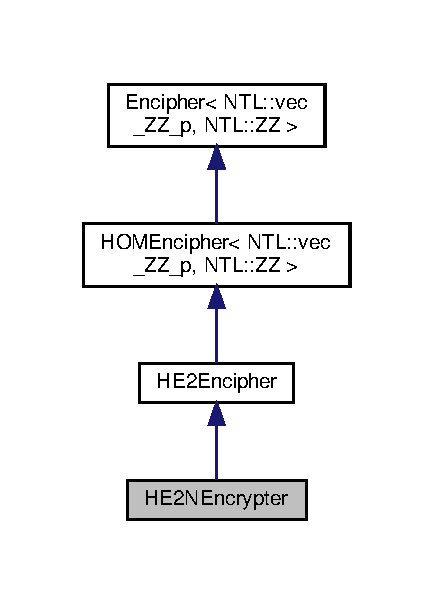
\includegraphics[width=208pt]{classHE2NEncrypter__inherit__graph}
\end{center}
\end{figure}


Collaboration diagram for H\+E2\+N\+Encrypter\+:
\nopagebreak
\begin{figure}[H]
\begin{center}
\leavevmode
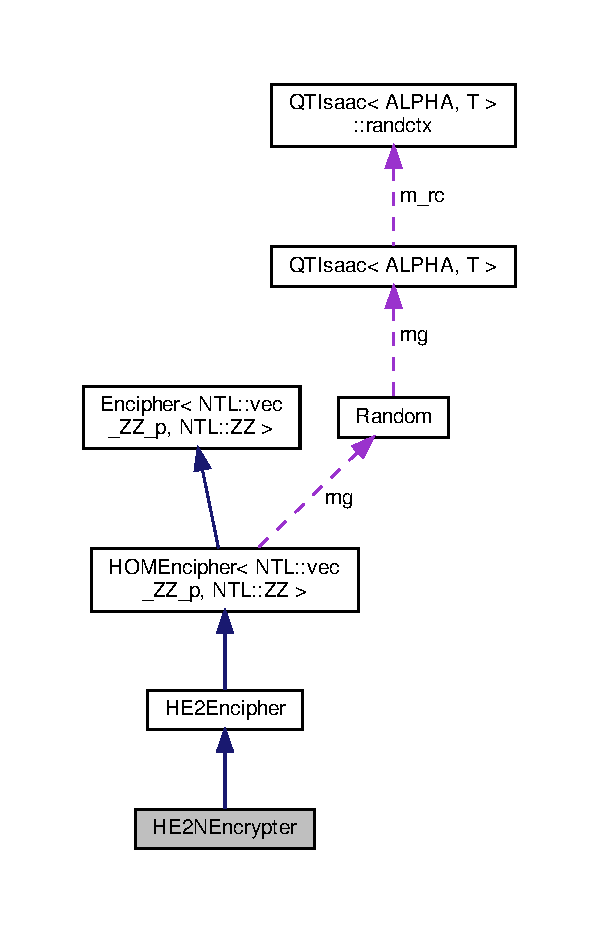
\includegraphics[width=288pt]{classHE2NEncrypter__coll__graph}
\end{center}
\end{figure}
\subsection*{Public Member Functions}
\begin{DoxyCompactItemize}
\item 
N\+T\+L\+::vec\+\_\+\+Z\+Z\+\_\+p \hyperlink{classHE2NEncrypter_aa7ae559f2407b7a5527bd42470224e1b}{encrypt} (N\+T\+L\+::\+ZZ \&plaintext) override
\item 
std\+::string \hyperlink{classHE2NEncrypter_a720d4ee52dadd55f61631554d2942a6b}{write\+Secrets\+To\+J\+S\+ON} () override
\item 
\hyperlink{classHE2NEncrypter_aa71432cbbe9565717fc5af638649d8d8}{H\+E2\+N\+Encrypter} (int lambda, int eta, int nu)
\item 
\hyperlink{classHE2NEncrypter_a3cb8269ce3f3de2f9a12d350366b36f9}{H\+E2\+N\+Encrypter} (int n, int d, int rho, int rhoprime)
\item 
virtual \hyperlink{classHE2NEncrypter_aa5ed36da105b7f9e4fa5fba012e37b0a}{$\sim$\+H\+E2\+N\+Encrypter} ()
\end{DoxyCompactItemize}
\subsection*{Private Attributes}
\begin{DoxyCompactItemize}
\item 
N\+T\+L\+::\+ZZ \hyperlink{classHE2NEncrypter_afd61d38d86bd894ba9e0b4f0bc6265b2}{kappa}
\item 
N\+T\+L\+::\+Z\+Z\+\_\+p $\ast$ \hyperlink{classHE2NEncrypter_ae13c7d0f1d11f2177f7183c50d0614a7}{kappamod}
\end{DoxyCompactItemize}
\subsection*{Additional Inherited Members}


\subsection{Constructor \& Destructor Documentation}
\mbox{\Hypertarget{classHE2NEncrypter_aa71432cbbe9565717fc5af638649d8d8}\label{classHE2NEncrypter_aa71432cbbe9565717fc5af638649d8d8}} 
\index{H\+E2\+N\+Encrypter@{H\+E2\+N\+Encrypter}!H\+E2\+N\+Encrypter@{H\+E2\+N\+Encrypter}}
\index{H\+E2\+N\+Encrypter@{H\+E2\+N\+Encrypter}!H\+E2\+N\+Encrypter@{H\+E2\+N\+Encrypter}}
\subsubsection{\texorpdfstring{H\+E2\+N\+Encrypter()}{HE2NEncrypter()}\hspace{0.1cm}{\footnotesize\ttfamily [1/2]}}
{\footnotesize\ttfamily H\+E2\+N\+Encrypter\+::\+H\+E2\+N\+Encrypter (\begin{DoxyParamCaption}\item[{int}]{lambda,  }\item[{int}]{eta,  }\item[{int}]{nu }\end{DoxyParamCaption})}

\mbox{\Hypertarget{classHE2NEncrypter_a3cb8269ce3f3de2f9a12d350366b36f9}\label{classHE2NEncrypter_a3cb8269ce3f3de2f9a12d350366b36f9}} 
\index{H\+E2\+N\+Encrypter@{H\+E2\+N\+Encrypter}!H\+E2\+N\+Encrypter@{H\+E2\+N\+Encrypter}}
\index{H\+E2\+N\+Encrypter@{H\+E2\+N\+Encrypter}!H\+E2\+N\+Encrypter@{H\+E2\+N\+Encrypter}}
\subsubsection{\texorpdfstring{H\+E2\+N\+Encrypter()}{HE2NEncrypter()}\hspace{0.1cm}{\footnotesize\ttfamily [2/2]}}
{\footnotesize\ttfamily H\+E2\+N\+Encrypter\+::\+H\+E2\+N\+Encrypter (\begin{DoxyParamCaption}\item[{int}]{n,  }\item[{int}]{d,  }\item[{int}]{rho,  }\item[{int}]{rhoprime }\end{DoxyParamCaption})}

\mbox{\Hypertarget{classHE2NEncrypter_aa5ed36da105b7f9e4fa5fba012e37b0a}\label{classHE2NEncrypter_aa5ed36da105b7f9e4fa5fba012e37b0a}} 
\index{H\+E2\+N\+Encrypter@{H\+E2\+N\+Encrypter}!````~H\+E2\+N\+Encrypter@{$\sim$\+H\+E2\+N\+Encrypter}}
\index{````~H\+E2\+N\+Encrypter@{$\sim$\+H\+E2\+N\+Encrypter}!H\+E2\+N\+Encrypter@{H\+E2\+N\+Encrypter}}
\subsubsection{\texorpdfstring{$\sim$\+H\+E2\+N\+Encrypter()}{~HE2NEncrypter()}}
{\footnotesize\ttfamily H\+E2\+N\+Encrypter\+::$\sim$\+H\+E2\+N\+Encrypter (\begin{DoxyParamCaption}{ }\end{DoxyParamCaption})\hspace{0.3cm}{\ttfamily [virtual]}}



\subsection{Member Function Documentation}
\mbox{\Hypertarget{classHE2NEncrypter_aa7ae559f2407b7a5527bd42470224e1b}\label{classHE2NEncrypter_aa7ae559f2407b7a5527bd42470224e1b}} 
\index{H\+E2\+N\+Encrypter@{H\+E2\+N\+Encrypter}!encrypt@{encrypt}}
\index{encrypt@{encrypt}!H\+E2\+N\+Encrypter@{H\+E2\+N\+Encrypter}}
\subsubsection{\texorpdfstring{encrypt()}{encrypt()}}
{\footnotesize\ttfamily N\+T\+L\+::vec\+\_\+\+Z\+Z\+\_\+p H\+E2\+N\+Encrypter\+::encrypt (\begin{DoxyParamCaption}\item[{N\+T\+L\+::\+ZZ \&}]{plaintext }\end{DoxyParamCaption})\hspace{0.3cm}{\ttfamily [override]}, {\ttfamily [virtual]}}



Implements \hyperlink{classEncipher_aaf8138eb280608bfd03c6eb762ffc010}{Encipher$<$ N\+T\+L\+::vec\+\_\+\+Z\+Z\+\_\+p, N\+T\+L\+::\+Z\+Z $>$}.

\mbox{\Hypertarget{classHE2NEncrypter_a720d4ee52dadd55f61631554d2942a6b}\label{classHE2NEncrypter_a720d4ee52dadd55f61631554d2942a6b}} 
\index{H\+E2\+N\+Encrypter@{H\+E2\+N\+Encrypter}!write\+Secrets\+To\+J\+S\+ON@{write\+Secrets\+To\+J\+S\+ON}}
\index{write\+Secrets\+To\+J\+S\+ON@{write\+Secrets\+To\+J\+S\+ON}!H\+E2\+N\+Encrypter@{H\+E2\+N\+Encrypter}}
\subsubsection{\texorpdfstring{write\+Secrets\+To\+J\+S\+O\+N()}{writeSecretsToJSON()}}
{\footnotesize\ttfamily std\+::string H\+E2\+N\+Encrypter\+::write\+Secrets\+To\+J\+S\+ON (\begin{DoxyParamCaption}{ }\end{DoxyParamCaption})\hspace{0.3cm}{\ttfamily [override]}, {\ttfamily [virtual]}}



Implements \hyperlink{classEncipher_a27d3efa1e364c1f0d7def65454c61b85}{Encipher$<$ N\+T\+L\+::vec\+\_\+\+Z\+Z\+\_\+p, N\+T\+L\+::\+Z\+Z $>$}.



\subsection{Member Data Documentation}
\mbox{\Hypertarget{classHE2NEncrypter_afd61d38d86bd894ba9e0b4f0bc6265b2}\label{classHE2NEncrypter_afd61d38d86bd894ba9e0b4f0bc6265b2}} 
\index{H\+E2\+N\+Encrypter@{H\+E2\+N\+Encrypter}!kappa@{kappa}}
\index{kappa@{kappa}!H\+E2\+N\+Encrypter@{H\+E2\+N\+Encrypter}}
\subsubsection{\texorpdfstring{kappa}{kappa}}
{\footnotesize\ttfamily N\+T\+L\+::\+ZZ H\+E2\+N\+Encrypter\+::kappa\hspace{0.3cm}{\ttfamily [private]}}

\mbox{\Hypertarget{classHE2NEncrypter_ae13c7d0f1d11f2177f7183c50d0614a7}\label{classHE2NEncrypter_ae13c7d0f1d11f2177f7183c50d0614a7}} 
\index{H\+E2\+N\+Encrypter@{H\+E2\+N\+Encrypter}!kappamod@{kappamod}}
\index{kappamod@{kappamod}!H\+E2\+N\+Encrypter@{H\+E2\+N\+Encrypter}}
\subsubsection{\texorpdfstring{kappamod}{kappamod}}
{\footnotesize\ttfamily N\+T\+L\+::\+Z\+Z\+\_\+p$\ast$ H\+E2\+N\+Encrypter\+::kappamod\hspace{0.3cm}{\ttfamily [private]}}



The documentation for this class was generated from the following files\+:\begin{DoxyCompactItemize}
\item 
include/\hyperlink{HE2NEncrypter_8h}{H\+E2\+N\+Encrypter.\+h}\item 
src/\hyperlink{HE2NEncrypter_8cpp}{H\+E2\+N\+Encrypter.\+cpp}\end{DoxyCompactItemize}

\hypertarget{classHOMDecipher}{}\section{H\+O\+M\+Decipher$<$ C, P $>$ Class Template Reference}
\label{classHOMDecipher}\index{H\+O\+M\+Decipher$<$ C, P $>$@{H\+O\+M\+Decipher$<$ C, P $>$}}


{\ttfamily \#include $<$H\+O\+M\+Decipher.\+hpp$>$}



Inheritance diagram for H\+O\+M\+Decipher$<$ C, P $>$\+:\nopagebreak
\begin{figure}[H]
\begin{center}
\leavevmode
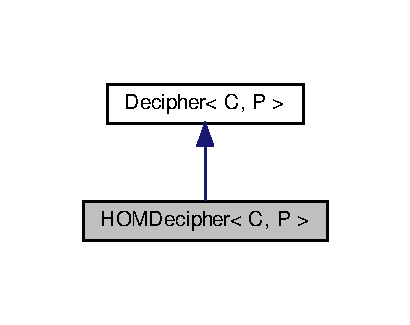
\includegraphics[width=197pt]{classHOMDecipher__inherit__graph}
\end{center}
\end{figure}


Collaboration diagram for H\+O\+M\+Decipher$<$ C, P $>$\+:\nopagebreak
\begin{figure}[H]
\begin{center}
\leavevmode
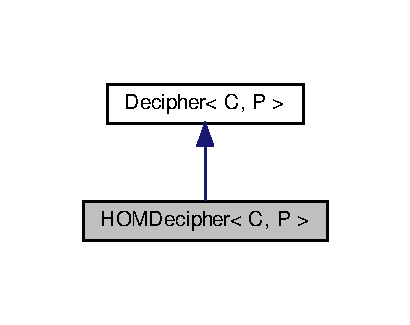
\includegraphics[width=197pt]{classHOMDecipher__coll__graph}
\end{center}
\end{figure}
\subsection*{Public Member Functions}
\begin{DoxyCompactItemize}
\item 
\hyperlink{classHOMDecipher_ab98e34714b534c4e02d08d952befa62b}{H\+O\+M\+Decipher} ()
\item 
virtual \hyperlink{classHOMDecipher_ae9f58f01719a48d5bbd41824181e181a}{$\sim$\+H\+O\+M\+Decipher} ()
\end{DoxyCompactItemize}
\subsection*{Protected Attributes}
\begin{DoxyCompactItemize}
\item 
N\+T\+L\+::\+ZZ \hyperlink{classHOMDecipher_a434f26bd73b3f9ee8bf999278d78a26c}{p}
\end{DoxyCompactItemize}


\subsection{Detailed Description}
\subsubsection*{template$<$typename C, typename P$>$\newline
class H\+O\+M\+Decipher$<$ C, P $>$}

This interface details the class members common to all HE{\itshape x} algorithms. All HE{\itshape x} decryption classes derive from this class. 
\begin{DoxyTemplParams}{Template Parameters}
{\em C} & Ciphertext type \\
\hline
{\em P} & Plaintext type \\
\hline
\end{DoxyTemplParams}


\subsection{Constructor \& Destructor Documentation}
\mbox{\Hypertarget{classHOMDecipher_ab98e34714b534c4e02d08d952befa62b}\label{classHOMDecipher_ab98e34714b534c4e02d08d952befa62b}} 
\index{H\+O\+M\+Decipher@{H\+O\+M\+Decipher}!H\+O\+M\+Decipher@{H\+O\+M\+Decipher}}
\index{H\+O\+M\+Decipher@{H\+O\+M\+Decipher}!H\+O\+M\+Decipher@{H\+O\+M\+Decipher}}
\subsubsection{\texorpdfstring{H\+O\+M\+Decipher()}{HOMDecipher()}}
{\footnotesize\ttfamily template$<$typename C, typename P$>$ \\
\hyperlink{classHOMDecipher}{H\+O\+M\+Decipher}$<$ C, P $>$\+::\hyperlink{classHOMDecipher}{H\+O\+M\+Decipher} (\begin{DoxyParamCaption}{ }\end{DoxyParamCaption})\hspace{0.3cm}{\ttfamily [inline]}}

\mbox{\Hypertarget{classHOMDecipher_ae9f58f01719a48d5bbd41824181e181a}\label{classHOMDecipher_ae9f58f01719a48d5bbd41824181e181a}} 
\index{H\+O\+M\+Decipher@{H\+O\+M\+Decipher}!````~H\+O\+M\+Decipher@{$\sim$\+H\+O\+M\+Decipher}}
\index{````~H\+O\+M\+Decipher@{$\sim$\+H\+O\+M\+Decipher}!H\+O\+M\+Decipher@{H\+O\+M\+Decipher}}
\subsubsection{\texorpdfstring{$\sim$\+H\+O\+M\+Decipher()}{~HOMDecipher()}}
{\footnotesize\ttfamily template$<$typename C, typename P$>$ \\
virtual \hyperlink{classHOMDecipher}{H\+O\+M\+Decipher}$<$ C, P $>$\+::$\sim$\hyperlink{classHOMDecipher}{H\+O\+M\+Decipher} (\begin{DoxyParamCaption}{ }\end{DoxyParamCaption})\hspace{0.3cm}{\ttfamily [inline]}, {\ttfamily [virtual]}}



\subsection{Member Data Documentation}
\mbox{\Hypertarget{classHOMDecipher_a434f26bd73b3f9ee8bf999278d78a26c}\label{classHOMDecipher_a434f26bd73b3f9ee8bf999278d78a26c}} 
\index{H\+O\+M\+Decipher@{H\+O\+M\+Decipher}!p@{p}}
\index{p@{p}!H\+O\+M\+Decipher@{H\+O\+M\+Decipher}}
\subsubsection{\texorpdfstring{p}{p}}
{\footnotesize\ttfamily template$<$typename C, typename P$>$ \\
N\+T\+L\+::\+ZZ \hyperlink{classHOMDecipher}{H\+O\+M\+Decipher}$<$ C, P $>$\+::p\hspace{0.3cm}{\ttfamily [protected]}}

Secret cipher parameter 

The documentation for this class was generated from the following file\+:\begin{DoxyCompactItemize}
\item 
include/\hyperlink{HOMDecipher_8hpp}{H\+O\+M\+Decipher.\+hpp}\end{DoxyCompactItemize}

\hypertarget{classHOMEncipher}{}\section{H\+O\+M\+Encipher$<$ C, P $>$ Class Template Reference}
\label{classHOMEncipher}\index{H\+O\+M\+Encipher$<$ C, P $>$@{H\+O\+M\+Encipher$<$ C, P $>$}}


{\ttfamily \#include $<$H\+O\+M\+Encipher.\+hpp$>$}



Inheritance diagram for H\+O\+M\+Encipher$<$ C, P $>$\+:
\nopagebreak
\begin{figure}[H]
\begin{center}
\leavevmode
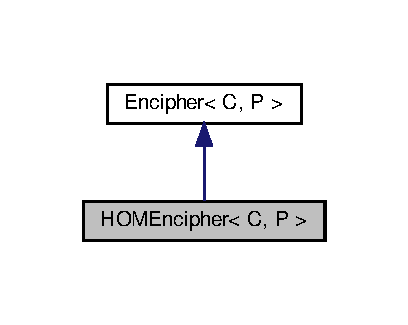
\includegraphics[width=196pt]{classHOMEncipher__inherit__graph}
\end{center}
\end{figure}


Collaboration diagram for H\+O\+M\+Encipher$<$ C, P $>$\+:
\nopagebreak
\begin{figure}[H]
\begin{center}
\leavevmode
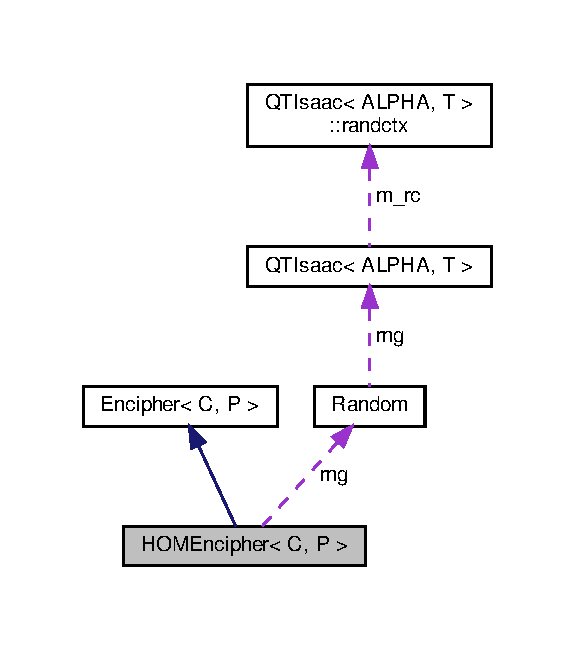
\includegraphics[width=276pt]{classHOMEncipher__coll__graph}
\end{center}
\end{figure}
\subsection*{Public Member Functions}
\begin{DoxyCompactItemize}
\item 
void \hyperlink{classHOMEncipher_aefdaccfe94ca8bd67a3ed1f5f045b04a}{init} ()
\item 
N\+T\+L\+::\+ZZ \hyperlink{classHOMEncipher_a43f920fd7feb8f3c9c6532c4935a6922}{get\+Modulus} ()
\item 
virtual std\+::string \hyperlink{classHOMEncipher_abf176e3fb85de6f0f6a2c96563397d39}{write\+Parameters\+To\+J\+S\+ON} ()=0
\item 
\hyperlink{classHOMEncipher_a08c76156f4f64433ead6ed2a1f142ffe}{H\+O\+M\+Encipher} ()
\item 
virtual \hyperlink{classHOMEncipher_a93b5c48425b0ac327757795703ecd2d7}{$\sim$\+H\+O\+M\+Encipher} ()
\end{DoxyCompactItemize}
\subsection*{Protected Member Functions}
\begin{DoxyCompactItemize}
\item 
void \hyperlink{classHOMEncipher_a6a715a6beed3174acc8d812d570462ca}{generate\+Modulus} (int lambda, int eta)
\end{DoxyCompactItemize}
\subsection*{Protected Attributes}
\begin{DoxyCompactItemize}
\item 
N\+T\+L\+::\+ZZ \hyperlink{classHOMEncipher_aa645061096356f6e2fd5ad3f0dfc1fc1}{modulus}
\item 
N\+T\+L\+::\+ZZ \hyperlink{classHOMEncipher_a57eb1b665612ec7caaa601af9b809866}{p}
\item 
N\+T\+L\+::\+ZZ \hyperlink{classHOMEncipher_ab9e6d7d4d4574c74a08169441e3213b2}{q}
\item 
\hyperlink{classRandom}{Random} $\ast$ \hyperlink{classHOMEncipher_a93a3cf6c4d8c7105380a2b13a08db774}{rng}
\end{DoxyCompactItemize}


\subsection{Constructor \& Destructor Documentation}
\mbox{\Hypertarget{classHOMEncipher_a08c76156f4f64433ead6ed2a1f142ffe}\label{classHOMEncipher_a08c76156f4f64433ead6ed2a1f142ffe}} 
\index{H\+O\+M\+Encipher@{H\+O\+M\+Encipher}!H\+O\+M\+Encipher@{H\+O\+M\+Encipher}}
\index{H\+O\+M\+Encipher@{H\+O\+M\+Encipher}!H\+O\+M\+Encipher@{H\+O\+M\+Encipher}}
\subsubsection{\texorpdfstring{H\+O\+M\+Encipher()}{HOMEncipher()}}
{\footnotesize\ttfamily template$<$typename C, typename P$>$ \\
\hyperlink{classHOMEncipher}{H\+O\+M\+Encipher}$<$ C, P $>$\+::\hyperlink{classHOMEncipher}{H\+O\+M\+Encipher} (\begin{DoxyParamCaption}{ }\end{DoxyParamCaption})\hspace{0.3cm}{\ttfamily [inline]}}

\mbox{\Hypertarget{classHOMEncipher_a93b5c48425b0ac327757795703ecd2d7}\label{classHOMEncipher_a93b5c48425b0ac327757795703ecd2d7}} 
\index{H\+O\+M\+Encipher@{H\+O\+M\+Encipher}!````~H\+O\+M\+Encipher@{$\sim$\+H\+O\+M\+Encipher}}
\index{````~H\+O\+M\+Encipher@{$\sim$\+H\+O\+M\+Encipher}!H\+O\+M\+Encipher@{H\+O\+M\+Encipher}}
\subsubsection{\texorpdfstring{$\sim$\+H\+O\+M\+Encipher()}{~HOMEncipher()}}
{\footnotesize\ttfamily template$<$typename C, typename P$>$ \\
virtual \hyperlink{classHOMEncipher}{H\+O\+M\+Encipher}$<$ C, P $>$\+::$\sim$\hyperlink{classHOMEncipher}{H\+O\+M\+Encipher} (\begin{DoxyParamCaption}{ }\end{DoxyParamCaption})\hspace{0.3cm}{\ttfamily [inline]}, {\ttfamily [virtual]}}



\subsection{Member Function Documentation}
\mbox{\Hypertarget{classHOMEncipher_a6a715a6beed3174acc8d812d570462ca}\label{classHOMEncipher_a6a715a6beed3174acc8d812d570462ca}} 
\index{H\+O\+M\+Encipher@{H\+O\+M\+Encipher}!generate\+Modulus@{generate\+Modulus}}
\index{generate\+Modulus@{generate\+Modulus}!H\+O\+M\+Encipher@{H\+O\+M\+Encipher}}
\subsubsection{\texorpdfstring{generate\+Modulus()}{generateModulus()}}
{\footnotesize\ttfamily template$<$typename C, typename P$>$ \\
void \hyperlink{classHOMEncipher}{H\+O\+M\+Encipher}$<$ C, P $>$\+::generate\+Modulus (\begin{DoxyParamCaption}\item[{int}]{lambda,  }\item[{int}]{eta }\end{DoxyParamCaption})\hspace{0.3cm}{\ttfamily [inline]}, {\ttfamily [protected]}}

\mbox{\Hypertarget{classHOMEncipher_a43f920fd7feb8f3c9c6532c4935a6922}\label{classHOMEncipher_a43f920fd7feb8f3c9c6532c4935a6922}} 
\index{H\+O\+M\+Encipher@{H\+O\+M\+Encipher}!get\+Modulus@{get\+Modulus}}
\index{get\+Modulus@{get\+Modulus}!H\+O\+M\+Encipher@{H\+O\+M\+Encipher}}
\subsubsection{\texorpdfstring{get\+Modulus()}{getModulus()}}
{\footnotesize\ttfamily template$<$typename C, typename P$>$ \\
N\+T\+L\+::\+ZZ \hyperlink{classHOMEncipher}{H\+O\+M\+Encipher}$<$ C, P $>$\+::get\+Modulus (\begin{DoxyParamCaption}{ }\end{DoxyParamCaption})\hspace{0.3cm}{\ttfamily [inline]}}

\mbox{\Hypertarget{classHOMEncipher_aefdaccfe94ca8bd67a3ed1f5f045b04a}\label{classHOMEncipher_aefdaccfe94ca8bd67a3ed1f5f045b04a}} 
\index{H\+O\+M\+Encipher@{H\+O\+M\+Encipher}!init@{init}}
\index{init@{init}!H\+O\+M\+Encipher@{H\+O\+M\+Encipher}}
\subsubsection{\texorpdfstring{init()}{init()}}
{\footnotesize\ttfamily template$<$typename C, typename P$>$ \\
void \hyperlink{classHOMEncipher}{H\+O\+M\+Encipher}$<$ C, P $>$\+::init (\begin{DoxyParamCaption}{ }\end{DoxyParamCaption})\hspace{0.3cm}{\ttfamily [inline]}}

\mbox{\Hypertarget{classHOMEncipher_abf176e3fb85de6f0f6a2c96563397d39}\label{classHOMEncipher_abf176e3fb85de6f0f6a2c96563397d39}} 
\index{H\+O\+M\+Encipher@{H\+O\+M\+Encipher}!write\+Parameters\+To\+J\+S\+ON@{write\+Parameters\+To\+J\+S\+ON}}
\index{write\+Parameters\+To\+J\+S\+ON@{write\+Parameters\+To\+J\+S\+ON}!H\+O\+M\+Encipher@{H\+O\+M\+Encipher}}
\subsubsection{\texorpdfstring{write\+Parameters\+To\+J\+S\+O\+N()}{writeParametersToJSON()}}
{\footnotesize\ttfamily template$<$typename C, typename P$>$ \\
virtual std\+::string \hyperlink{classHOMEncipher}{H\+O\+M\+Encipher}$<$ C, P $>$\+::write\+Parameters\+To\+J\+S\+ON (\begin{DoxyParamCaption}{ }\end{DoxyParamCaption})\hspace{0.3cm}{\ttfamily [pure virtual]}}



Implemented in \hyperlink{classHE2Encipher_a802a75d83bb833bf458a1e89792026bc}{H\+E2\+Encipher}, and \hyperlink{classHE1Encipher_a0aa1ef94d9147591367dbbc6ce03e5e1}{H\+E1\+Encipher}.



\subsection{Member Data Documentation}
\mbox{\Hypertarget{classHOMEncipher_aa645061096356f6e2fd5ad3f0dfc1fc1}\label{classHOMEncipher_aa645061096356f6e2fd5ad3f0dfc1fc1}} 
\index{H\+O\+M\+Encipher@{H\+O\+M\+Encipher}!modulus@{modulus}}
\index{modulus@{modulus}!H\+O\+M\+Encipher@{H\+O\+M\+Encipher}}
\subsubsection{\texorpdfstring{modulus}{modulus}}
{\footnotesize\ttfamily template$<$typename C, typename P$>$ \\
N\+T\+L\+::\+ZZ \hyperlink{classHOMEncipher}{H\+O\+M\+Encipher}$<$ C, P $>$\+::modulus\hspace{0.3cm}{\ttfamily [protected]}}

\mbox{\Hypertarget{classHOMEncipher_a57eb1b665612ec7caaa601af9b809866}\label{classHOMEncipher_a57eb1b665612ec7caaa601af9b809866}} 
\index{H\+O\+M\+Encipher@{H\+O\+M\+Encipher}!p@{p}}
\index{p@{p}!H\+O\+M\+Encipher@{H\+O\+M\+Encipher}}
\subsubsection{\texorpdfstring{p}{p}}
{\footnotesize\ttfamily template$<$typename C, typename P$>$ \\
N\+T\+L\+::\+ZZ \hyperlink{classHOMEncipher}{H\+O\+M\+Encipher}$<$ C, P $>$\+::p\hspace{0.3cm}{\ttfamily [protected]}}

\mbox{\Hypertarget{classHOMEncipher_ab9e6d7d4d4574c74a08169441e3213b2}\label{classHOMEncipher_ab9e6d7d4d4574c74a08169441e3213b2}} 
\index{H\+O\+M\+Encipher@{H\+O\+M\+Encipher}!q@{q}}
\index{q@{q}!H\+O\+M\+Encipher@{H\+O\+M\+Encipher}}
\subsubsection{\texorpdfstring{q}{q}}
{\footnotesize\ttfamily template$<$typename C, typename P$>$ \\
N\+T\+L\+::\+ZZ \hyperlink{classHOMEncipher}{H\+O\+M\+Encipher}$<$ C, P $>$\+::q\hspace{0.3cm}{\ttfamily [protected]}}

\mbox{\Hypertarget{classHOMEncipher_a93a3cf6c4d8c7105380a2b13a08db774}\label{classHOMEncipher_a93a3cf6c4d8c7105380a2b13a08db774}} 
\index{H\+O\+M\+Encipher@{H\+O\+M\+Encipher}!rng@{rng}}
\index{rng@{rng}!H\+O\+M\+Encipher@{H\+O\+M\+Encipher}}
\subsubsection{\texorpdfstring{rng}{rng}}
{\footnotesize\ttfamily template$<$typename C, typename P$>$ \\
\hyperlink{classRandom}{Random}$\ast$ \hyperlink{classHOMEncipher}{H\+O\+M\+Encipher}$<$ C, P $>$\+::rng\hspace{0.3cm}{\ttfamily [protected]}}



The documentation for this class was generated from the following file\+:\begin{DoxyCompactItemize}
\item 
include/\hyperlink{HOMEncipher_8hpp}{H\+O\+M\+Encipher.\+hpp}\end{DoxyCompactItemize}

\hypertarget{classPolyACDDecrypter}{}\section{Poly\+A\+C\+D\+Decrypter Class Reference}
\label{classPolyACDDecrypter}\index{Poly\+A\+C\+D\+Decrypter@{Poly\+A\+C\+D\+Decrypter}}


{\ttfamily \#include $<$Poly\+A\+C\+D\+Decrypter.\+h$>$}



Inheritance diagram for Poly\+A\+C\+D\+Decrypter\+:\nopagebreak
\begin{figure}[H]
\begin{center}
\leavevmode
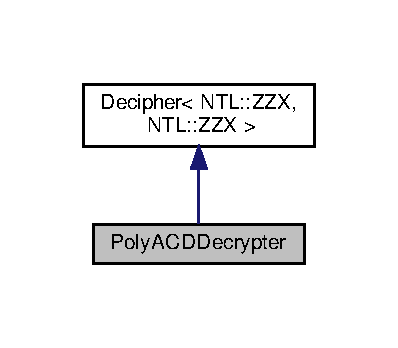
\includegraphics[width=191pt]{classPolyACDDecrypter__inherit__graph}
\end{center}
\end{figure}


Collaboration diagram for Poly\+A\+C\+D\+Decrypter\+:\nopagebreak
\begin{figure}[H]
\begin{center}
\leavevmode
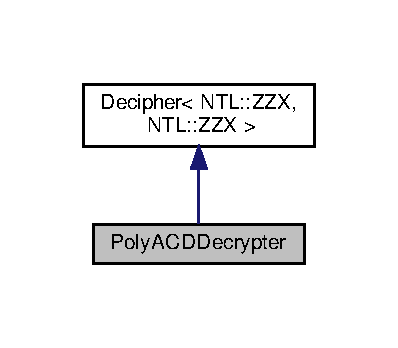
\includegraphics[width=191pt]{classPolyACDDecrypter__coll__graph}
\end{center}
\end{figure}
\subsection*{Public Member Functions}
\begin{DoxyCompactItemize}
\item 
\hyperlink{classPolyACDDecrypter_ad83cc12ab1b782090b0d14489e5e114c}{Poly\+A\+C\+D\+Decrypter} ()
\item 
virtual \hyperlink{classPolyACDDecrypter_a91c523391a2d25bd27160ef045f19c79}{$\sim$\+Poly\+A\+C\+D\+Decrypter} ()
\item 
void \hyperlink{classPolyACDDecrypter_a55e7f81c6d8d10e00e072547ac68239a}{read\+Secrets\+From\+J\+S\+ON} (std\+::string \&string) override
\item 
N\+T\+L\+::\+Z\+ZX \hyperlink{classPolyACDDecrypter_a96626f2c267d9cc4b18ed25cb584d982}{decrypt} (N\+T\+L\+::\+Z\+ZX \&ciphertext) override
\end{DoxyCompactItemize}
\subsection*{Private Attributes}
\begin{DoxyCompactItemize}
\item 
N\+T\+L\+::\+ZZ \hyperlink{classPolyACDDecrypter_a86ca294cafa0cd5fa070d43127bd8c01}{k1}
\item 
N\+T\+L\+::\+Z\+ZX \hyperlink{classPolyACDDecrypter_a3b0967ca5e6df810ef952521eadefa44}{k2}
\end{DoxyCompactItemize}


\subsection{Constructor \& Destructor Documentation}
\mbox{\Hypertarget{classPolyACDDecrypter_ad83cc12ab1b782090b0d14489e5e114c}\label{classPolyACDDecrypter_ad83cc12ab1b782090b0d14489e5e114c}} 
\index{Poly\+A\+C\+D\+Decrypter@{Poly\+A\+C\+D\+Decrypter}!Poly\+A\+C\+D\+Decrypter@{Poly\+A\+C\+D\+Decrypter}}
\index{Poly\+A\+C\+D\+Decrypter@{Poly\+A\+C\+D\+Decrypter}!Poly\+A\+C\+D\+Decrypter@{Poly\+A\+C\+D\+Decrypter}}
\subsubsection{\texorpdfstring{Poly\+A\+C\+D\+Decrypter()}{PolyACDDecrypter()}}
{\footnotesize\ttfamily Poly\+A\+C\+D\+Decrypter\+::\+Poly\+A\+C\+D\+Decrypter (\begin{DoxyParamCaption}{ }\end{DoxyParamCaption})}

\mbox{\Hypertarget{classPolyACDDecrypter_a91c523391a2d25bd27160ef045f19c79}\label{classPolyACDDecrypter_a91c523391a2d25bd27160ef045f19c79}} 
\index{Poly\+A\+C\+D\+Decrypter@{Poly\+A\+C\+D\+Decrypter}!````~Poly\+A\+C\+D\+Decrypter@{$\sim$\+Poly\+A\+C\+D\+Decrypter}}
\index{````~Poly\+A\+C\+D\+Decrypter@{$\sim$\+Poly\+A\+C\+D\+Decrypter}!Poly\+A\+C\+D\+Decrypter@{Poly\+A\+C\+D\+Decrypter}}
\subsubsection{\texorpdfstring{$\sim$\+Poly\+A\+C\+D\+Decrypter()}{~PolyACDDecrypter()}}
{\footnotesize\ttfamily Poly\+A\+C\+D\+Decrypter\+::$\sim$\+Poly\+A\+C\+D\+Decrypter (\begin{DoxyParamCaption}{ }\end{DoxyParamCaption})\hspace{0.3cm}{\ttfamily [virtual]}}



\subsection{Member Function Documentation}
\mbox{\Hypertarget{classPolyACDDecrypter_a96626f2c267d9cc4b18ed25cb584d982}\label{classPolyACDDecrypter_a96626f2c267d9cc4b18ed25cb584d982}} 
\index{Poly\+A\+C\+D\+Decrypter@{Poly\+A\+C\+D\+Decrypter}!decrypt@{decrypt}}
\index{decrypt@{decrypt}!Poly\+A\+C\+D\+Decrypter@{Poly\+A\+C\+D\+Decrypter}}
\subsubsection{\texorpdfstring{decrypt()}{decrypt()}}
{\footnotesize\ttfamily N\+T\+L\+::\+Z\+ZX Poly\+A\+C\+D\+Decrypter\+::decrypt (\begin{DoxyParamCaption}\item[{N\+T\+L\+::\+Z\+ZX \&}]{ciphertext }\end{DoxyParamCaption})\hspace{0.3cm}{\ttfamily [override]}, {\ttfamily [virtual]}}

Decrypts a ciphertext 
\begin{DoxyParams}{Parameters}
{\em ciphertext} & Ciphertext value \\
\hline
\end{DoxyParams}
\begin{DoxyReturn}{Returns}
Plaintext value 
\end{DoxyReturn}


Implements \hyperlink{classDecipher_ac6b8c369eda2d7e17fa90cb594cf41b6}{Decipher$<$ N\+T\+L\+::\+Z\+Z\+X, N\+T\+L\+::\+Z\+Z\+X $>$}.

\mbox{\Hypertarget{classPolyACDDecrypter_a55e7f81c6d8d10e00e072547ac68239a}\label{classPolyACDDecrypter_a55e7f81c6d8d10e00e072547ac68239a}} 
\index{Poly\+A\+C\+D\+Decrypter@{Poly\+A\+C\+D\+Decrypter}!read\+Secrets\+From\+J\+S\+ON@{read\+Secrets\+From\+J\+S\+ON}}
\index{read\+Secrets\+From\+J\+S\+ON@{read\+Secrets\+From\+J\+S\+ON}!Poly\+A\+C\+D\+Decrypter@{Poly\+A\+C\+D\+Decrypter}}
\subsubsection{\texorpdfstring{read\+Secrets\+From\+J\+S\+O\+N()}{readSecretsFromJSON()}}
{\footnotesize\ttfamily void Poly\+A\+C\+D\+Decrypter\+::read\+Secrets\+From\+J\+S\+ON (\begin{DoxyParamCaption}\item[{std\+::string \&}]{string }\end{DoxyParamCaption})\hspace{0.3cm}{\ttfamily [override]}, {\ttfamily [virtual]}}

Reads the cipher secrets in from a J\+S\+ON string 
\begin{DoxyParams}{Parameters}
{\em string} & J\+S\+ON string \\
\hline
\end{DoxyParams}


Implements \hyperlink{classDecipher_a39aea002012130201e12a8fa7d84dda5}{Decipher$<$ N\+T\+L\+::\+Z\+Z\+X, N\+T\+L\+::\+Z\+Z\+X $>$}.



\subsection{Member Data Documentation}
\mbox{\Hypertarget{classPolyACDDecrypter_a86ca294cafa0cd5fa070d43127bd8c01}\label{classPolyACDDecrypter_a86ca294cafa0cd5fa070d43127bd8c01}} 
\index{Poly\+A\+C\+D\+Decrypter@{Poly\+A\+C\+D\+Decrypter}!k1@{k1}}
\index{k1@{k1}!Poly\+A\+C\+D\+Decrypter@{Poly\+A\+C\+D\+Decrypter}}
\subsubsection{\texorpdfstring{k1}{k1}}
{\footnotesize\ttfamily N\+T\+L\+::\+ZZ Poly\+A\+C\+D\+Decrypter\+::k1\hspace{0.3cm}{\ttfamily [private]}}

Secret large integer parameter \mbox{\Hypertarget{classPolyACDDecrypter_a3b0967ca5e6df810ef952521eadefa44}\label{classPolyACDDecrypter_a3b0967ca5e6df810ef952521eadefa44}} 
\index{Poly\+A\+C\+D\+Decrypter@{Poly\+A\+C\+D\+Decrypter}!k2@{k2}}
\index{k2@{k2}!Poly\+A\+C\+D\+Decrypter@{Poly\+A\+C\+D\+Decrypter}}
\subsubsection{\texorpdfstring{k2}{k2}}
{\footnotesize\ttfamily N\+T\+L\+::\+Z\+ZX Poly\+A\+C\+D\+Decrypter\+::k2\hspace{0.3cm}{\ttfamily [private]}}

Secret polynomial 

The documentation for this class was generated from the following files\+:\begin{DoxyCompactItemize}
\item 
include/\hyperlink{PolyACDDecrypter_8h}{Poly\+A\+C\+D\+Decrypter.\+h}\item 
src/\hyperlink{PolyACDDecrypter_8cpp}{Poly\+A\+C\+D\+Decrypter.\+cpp}\end{DoxyCompactItemize}

\hypertarget{classPolyACDEncrypter}{}\section{Poly\+A\+C\+D\+Encrypter Class Reference}
\label{classPolyACDEncrypter}\index{Poly\+A\+C\+D\+Encrypter@{Poly\+A\+C\+D\+Encrypter}}


{\ttfamily \#include $<$Poly\+A\+C\+D\+Encrypter.\+h$>$}



Inheritance diagram for Poly\+A\+C\+D\+Encrypter\+:\nopagebreak
\begin{figure}[H]
\begin{center}
\leavevmode
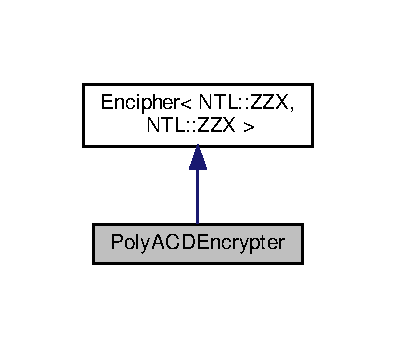
\includegraphics[width=190pt]{classPolyACDEncrypter__inherit__graph}
\end{center}
\end{figure}


Collaboration diagram for Poly\+A\+C\+D\+Encrypter\+:\nopagebreak
\begin{figure}[H]
\begin{center}
\leavevmode
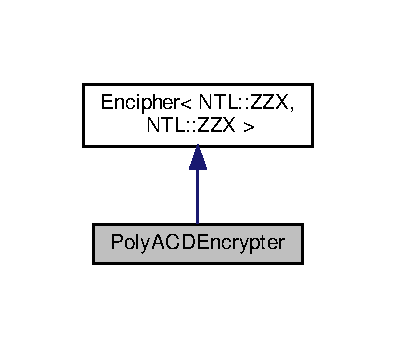
\includegraphics[width=190pt]{classPolyACDEncrypter__coll__graph}
\end{center}
\end{figure}
\subsection*{Public Member Functions}
\begin{DoxyCompactItemize}
\item 
\hyperlink{classPolyACDEncrypter_aa8129aeb902913825c980316157b33e4}{Poly\+A\+C\+D\+Encrypter} (int lambda, int \hyperlink{classPolyACDEncrypter_a3afaccbe1fbc6379e6061f1489e9a253}{mu}, int d)
\item 
\hyperlink{classPolyACDEncrypter_abae92af62b71ad8f52e786a4263f981f}{Poly\+A\+C\+D\+Encrypter} (int \hyperlink{classPolyACDEncrypter_a3afaccbe1fbc6379e6061f1489e9a253}{mu}, std\+::string \&secrets)
\item 
virtual \hyperlink{classPolyACDEncrypter_a63824228dbc9c64ccdbddc154069592b}{$\sim$\+Poly\+A\+C\+D\+Encrypter} ()
\item 
N\+T\+L\+::\+Z\+ZX \hyperlink{classPolyACDEncrypter_a5233a73398d39d93567392c64a120e1e}{encrypt} (N\+T\+L\+::\+Z\+ZX \&plaintext) override
\item 
N\+T\+L\+::\+Z\+ZX \hyperlink{classPolyACDEncrypter_ae4de72005efe6dc0dca2d2b41a655b3a}{encrypt} (N\+T\+L\+::vec\+\_\+\+ZZ \&plaintext)
\item 
std\+::string \hyperlink{classPolyACDEncrypter_af478f2fe3f886d23749955eaa72e413b}{write\+Secrets\+To\+J\+S\+ON} () override
\end{DoxyCompactItemize}
\subsection*{Private Attributes}
\begin{DoxyCompactItemize}
\item 
N\+T\+L\+::\+ZZ \hyperlink{classPolyACDEncrypter_a198e96b474e1a02590aeb55d7fe348d7}{k1}
\item 
N\+T\+L\+::\+Z\+ZX \hyperlink{classPolyACDEncrypter_aa4de2f8e1e03808b7a7c7b9576084482}{k2}
\item 
int \hyperlink{classPolyACDEncrypter_a3afaccbe1fbc6379e6061f1489e9a253}{mu}
\end{DoxyCompactItemize}


\subsection{Constructor \& Destructor Documentation}
\mbox{\Hypertarget{classPolyACDEncrypter_aa8129aeb902913825c980316157b33e4}\label{classPolyACDEncrypter_aa8129aeb902913825c980316157b33e4}} 
\index{Poly\+A\+C\+D\+Encrypter@{Poly\+A\+C\+D\+Encrypter}!Poly\+A\+C\+D\+Encrypter@{Poly\+A\+C\+D\+Encrypter}}
\index{Poly\+A\+C\+D\+Encrypter@{Poly\+A\+C\+D\+Encrypter}!Poly\+A\+C\+D\+Encrypter@{Poly\+A\+C\+D\+Encrypter}}
\subsubsection{\texorpdfstring{Poly\+A\+C\+D\+Encrypter()}{PolyACDEncrypter()}\hspace{0.1cm}{\footnotesize\ttfamily [1/2]}}
{\footnotesize\ttfamily Poly\+A\+C\+D\+Encrypter\+::\+Poly\+A\+C\+D\+Encrypter (\begin{DoxyParamCaption}\item[{int}]{lambda,  }\item[{int}]{mu,  }\item[{int}]{d }\end{DoxyParamCaption})}

\mbox{\Hypertarget{classPolyACDEncrypter_abae92af62b71ad8f52e786a4263f981f}\label{classPolyACDEncrypter_abae92af62b71ad8f52e786a4263f981f}} 
\index{Poly\+A\+C\+D\+Encrypter@{Poly\+A\+C\+D\+Encrypter}!Poly\+A\+C\+D\+Encrypter@{Poly\+A\+C\+D\+Encrypter}}
\index{Poly\+A\+C\+D\+Encrypter@{Poly\+A\+C\+D\+Encrypter}!Poly\+A\+C\+D\+Encrypter@{Poly\+A\+C\+D\+Encrypter}}
\subsubsection{\texorpdfstring{Poly\+A\+C\+D\+Encrypter()}{PolyACDEncrypter()}\hspace{0.1cm}{\footnotesize\ttfamily [2/2]}}
{\footnotesize\ttfamily Poly\+A\+C\+D\+Encrypter\+::\+Poly\+A\+C\+D\+Encrypter (\begin{DoxyParamCaption}\item[{int}]{mu,  }\item[{std\+::string \&}]{secrets }\end{DoxyParamCaption})}

\mbox{\Hypertarget{classPolyACDEncrypter_a63824228dbc9c64ccdbddc154069592b}\label{classPolyACDEncrypter_a63824228dbc9c64ccdbddc154069592b}} 
\index{Poly\+A\+C\+D\+Encrypter@{Poly\+A\+C\+D\+Encrypter}!````~Poly\+A\+C\+D\+Encrypter@{$\sim$\+Poly\+A\+C\+D\+Encrypter}}
\index{````~Poly\+A\+C\+D\+Encrypter@{$\sim$\+Poly\+A\+C\+D\+Encrypter}!Poly\+A\+C\+D\+Encrypter@{Poly\+A\+C\+D\+Encrypter}}
\subsubsection{\texorpdfstring{$\sim$\+Poly\+A\+C\+D\+Encrypter()}{~PolyACDEncrypter()}}
{\footnotesize\ttfamily Poly\+A\+C\+D\+Encrypter\+::$\sim$\+Poly\+A\+C\+D\+Encrypter (\begin{DoxyParamCaption}{ }\end{DoxyParamCaption})\hspace{0.3cm}{\ttfamily [virtual]}}



\subsection{Member Function Documentation}
\mbox{\Hypertarget{classPolyACDEncrypter_a5233a73398d39d93567392c64a120e1e}\label{classPolyACDEncrypter_a5233a73398d39d93567392c64a120e1e}} 
\index{Poly\+A\+C\+D\+Encrypter@{Poly\+A\+C\+D\+Encrypter}!encrypt@{encrypt}}
\index{encrypt@{encrypt}!Poly\+A\+C\+D\+Encrypter@{Poly\+A\+C\+D\+Encrypter}}
\subsubsection{\texorpdfstring{encrypt()}{encrypt()}\hspace{0.1cm}{\footnotesize\ttfamily [1/2]}}
{\footnotesize\ttfamily N\+T\+L\+::\+Z\+ZX Poly\+A\+C\+D\+Encrypter\+::encrypt (\begin{DoxyParamCaption}\item[{N\+T\+L\+::\+Z\+ZX \&}]{plaintext }\end{DoxyParamCaption})\hspace{0.3cm}{\ttfamily [override]}, {\ttfamily [virtual]}}

Encrypt a plaintext 
\begin{DoxyParams}{Parameters}
{\em plaintext} & A plaintext value \\
\hline
\end{DoxyParams}
\begin{DoxyReturn}{Returns}
A ciphertext value 
\end{DoxyReturn}


Implements \hyperlink{classEncipher_aaf8138eb280608bfd03c6eb762ffc010}{Encipher$<$ N\+T\+L\+::\+Z\+Z\+X, N\+T\+L\+::\+Z\+Z\+X $>$}.

\mbox{\Hypertarget{classPolyACDEncrypter_ae4de72005efe6dc0dca2d2b41a655b3a}\label{classPolyACDEncrypter_ae4de72005efe6dc0dca2d2b41a655b3a}} 
\index{Poly\+A\+C\+D\+Encrypter@{Poly\+A\+C\+D\+Encrypter}!encrypt@{encrypt}}
\index{encrypt@{encrypt}!Poly\+A\+C\+D\+Encrypter@{Poly\+A\+C\+D\+Encrypter}}
\subsubsection{\texorpdfstring{encrypt()}{encrypt()}\hspace{0.1cm}{\footnotesize\ttfamily [2/2]}}
{\footnotesize\ttfamily N\+T\+L\+::\+Z\+ZX Poly\+A\+C\+D\+Encrypter\+::encrypt (\begin{DoxyParamCaption}\item[{N\+T\+L\+::vec\+\_\+\+ZZ \&}]{plaintext }\end{DoxyParamCaption})}

\mbox{\Hypertarget{classPolyACDEncrypter_af478f2fe3f886d23749955eaa72e413b}\label{classPolyACDEncrypter_af478f2fe3f886d23749955eaa72e413b}} 
\index{Poly\+A\+C\+D\+Encrypter@{Poly\+A\+C\+D\+Encrypter}!write\+Secrets\+To\+J\+S\+ON@{write\+Secrets\+To\+J\+S\+ON}}
\index{write\+Secrets\+To\+J\+S\+ON@{write\+Secrets\+To\+J\+S\+ON}!Poly\+A\+C\+D\+Encrypter@{Poly\+A\+C\+D\+Encrypter}}
\subsubsection{\texorpdfstring{write\+Secrets\+To\+J\+S\+O\+N()}{writeSecretsToJSON()}}
{\footnotesize\ttfamily std\+::string Poly\+A\+C\+D\+Encrypter\+::write\+Secrets\+To\+J\+S\+ON (\begin{DoxyParamCaption}{ }\end{DoxyParamCaption})\hspace{0.3cm}{\ttfamily [override]}, {\ttfamily [virtual]}}

Writes cipher secrets out to a J\+S\+ON string \begin{DoxyReturn}{Returns}
J\+S\+ON string 
\end{DoxyReturn}


Implements \hyperlink{classEncipher_a27d3efa1e364c1f0d7def65454c61b85}{Encipher$<$ N\+T\+L\+::\+Z\+Z\+X, N\+T\+L\+::\+Z\+Z\+X $>$}.



\subsection{Member Data Documentation}
\mbox{\Hypertarget{classPolyACDEncrypter_a198e96b474e1a02590aeb55d7fe348d7}\label{classPolyACDEncrypter_a198e96b474e1a02590aeb55d7fe348d7}} 
\index{Poly\+A\+C\+D\+Encrypter@{Poly\+A\+C\+D\+Encrypter}!k1@{k1}}
\index{k1@{k1}!Poly\+A\+C\+D\+Encrypter@{Poly\+A\+C\+D\+Encrypter}}
\subsubsection{\texorpdfstring{k1}{k1}}
{\footnotesize\ttfamily N\+T\+L\+::\+ZZ Poly\+A\+C\+D\+Encrypter\+::k1\hspace{0.3cm}{\ttfamily [private]}}

Secret large integer parameter \mbox{\Hypertarget{classPolyACDEncrypter_aa4de2f8e1e03808b7a7c7b9576084482}\label{classPolyACDEncrypter_aa4de2f8e1e03808b7a7c7b9576084482}} 
\index{Poly\+A\+C\+D\+Encrypter@{Poly\+A\+C\+D\+Encrypter}!k2@{k2}}
\index{k2@{k2}!Poly\+A\+C\+D\+Encrypter@{Poly\+A\+C\+D\+Encrypter}}
\subsubsection{\texorpdfstring{k2}{k2}}
{\footnotesize\ttfamily N\+T\+L\+::\+Z\+ZX Poly\+A\+C\+D\+Encrypter\+::k2\hspace{0.3cm}{\ttfamily [private]}}

Secret polynomial \mbox{\Hypertarget{classPolyACDEncrypter_a3afaccbe1fbc6379e6061f1489e9a253}\label{classPolyACDEncrypter_a3afaccbe1fbc6379e6061f1489e9a253}} 
\index{Poly\+A\+C\+D\+Encrypter@{Poly\+A\+C\+D\+Encrypter}!mu@{mu}}
\index{mu@{mu}!Poly\+A\+C\+D\+Encrypter@{Poly\+A\+C\+D\+Encrypter}}
\subsubsection{\texorpdfstring{mu}{mu}}
{\footnotesize\ttfamily int Poly\+A\+C\+D\+Encrypter\+::mu\hspace{0.3cm}{\ttfamily [private]}}

The bit length of the plaintext coefficients 

The documentation for this class was generated from the following files\+:\begin{DoxyCompactItemize}
\item 
include/\hyperlink{PolyACDEncrypter_8h}{Poly\+A\+C\+D\+Encrypter.\+h}\item 
src/\hyperlink{PolyACDEncrypter_8cpp}{Poly\+A\+C\+D\+Encrypter.\+cpp}\end{DoxyCompactItemize}

\hypertarget{classQTIsaac}{}\section{Q\+T\+Isaac$<$ A\+L\+P\+HA, T $>$ Class Template Reference}
\label{classQTIsaac}\index{Q\+T\+Isaac$<$ A\+L\+P\+H\+A, T $>$@{Q\+T\+Isaac$<$ A\+L\+P\+H\+A, T $>$}}


{\ttfamily \#include $<$isaac.\+hpp$>$}



Collaboration diagram for Q\+T\+Isaac$<$ A\+L\+P\+HA, T $>$\+:
\nopagebreak
\begin{figure}[H]
\begin{center}
\leavevmode
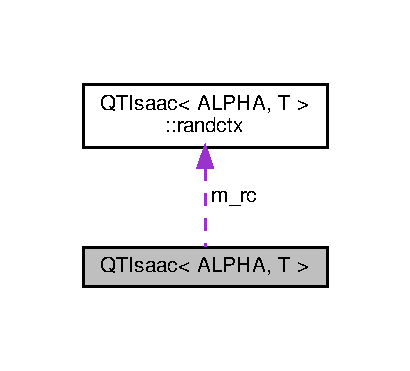
\includegraphics[width=197pt]{classQTIsaac__coll__graph}
\end{center}
\end{figure}
\subsection*{Classes}
\begin{DoxyCompactItemize}
\item 
struct \hyperlink{structQTIsaac_1_1randctx}{randctx}
\end{DoxyCompactItemize}
\subsection*{Public Types}
\begin{DoxyCompactItemize}
\item 
enum \{ \hyperlink{classQTIsaac_a2f9d908d12a5725146e161998b733233a44174520f740123b364728ca92b3dc97}{N} = (1$<$$<$A\+L\+P\+HA)
 \}
\item 
typedef unsigned char \hyperlink{classQTIsaac_a1f78939d0806ed6006253a9ead8052b3}{byte}
\end{DoxyCompactItemize}
\subsection*{Public Member Functions}
\begin{DoxyCompactItemize}
\item 
\hyperlink{classQTIsaac_afbf292ab78e041bd2bbd5066241d88c3}{Q\+T\+Isaac} (T a=0, T b=0, T c=0)
\item 
virtual \hyperlink{classQTIsaac_ab0dfe7af413f019311ec43aec83a0592}{$\sim$\+Q\+T\+Isaac} (void)
\item 
T \hyperlink{classQTIsaac_a43a34ab9819572127d4f13e7344b2a95}{rand} (void)
\item 
virtual void \hyperlink{classQTIsaac_a5d1004b08f22ef74794597d139ca31b7}{randinit} (\hyperlink{structQTIsaac_1_1randctx}{randctx} $\ast$ctx, bool b\+Use\+Seed)
\item 
virtual void \hyperlink{classQTIsaac_ae8ec04439ce5f24bb3b337065f9148a9}{srand} (T a=0, T b=0, T c=0, T $\ast$s=nullptr)
\end{DoxyCompactItemize}
\subsection*{Protected Member Functions}
\begin{DoxyCompactItemize}
\item 
virtual void \hyperlink{classQTIsaac_aa92e5e94f65d61e9395664dc5d2cf9b3}{isaac} (\hyperlink{structQTIsaac_1_1randctx}{randctx} $\ast$ctx)
\item 
T \hyperlink{classQTIsaac_a4b1bca72fa71e1ee79c285047e55a469}{ind} (T $\ast$mm, T x)
\item 
void \hyperlink{classQTIsaac_a97aee0e8269aa92acc9237dff6a8a370}{rngstep} (T mix, T \&a, T \&b, T $\ast$\&mm, T $\ast$\&m, T $\ast$\&m2, T $\ast$\&r, T \&x, T \&y)
\item 
virtual void \hyperlink{classQTIsaac_a9eb2ef09b2864b5b2b0406b7d0236ade}{shuffle} (T \&a, T \&b, T \&c, T \&d, T \&e, T \&f, T \&g, T \&h)
\end{DoxyCompactItemize}
\subsection*{Private Attributes}
\begin{DoxyCompactItemize}
\item 
\hyperlink{structQTIsaac_1_1randctx}{randctx} \hyperlink{classQTIsaac_a7eb189761ac0cd7dea189572e544cb9a}{m\+\_\+rc}
\end{DoxyCompactItemize}


\subsection{Member Typedef Documentation}
\mbox{\Hypertarget{classQTIsaac_a1f78939d0806ed6006253a9ead8052b3}\label{classQTIsaac_a1f78939d0806ed6006253a9ead8052b3}} 
\index{Q\+T\+Isaac@{Q\+T\+Isaac}!byte@{byte}}
\index{byte@{byte}!Q\+T\+Isaac@{Q\+T\+Isaac}}
\subsubsection{\texorpdfstring{byte}{byte}}
{\footnotesize\ttfamily template$<$int A\+L\+P\+HA = (8), class T = I\+S\+A\+A\+C\+\_\+\+I\+NT$>$ \\
typedef unsigned char \hyperlink{classQTIsaac}{Q\+T\+Isaac}$<$ A\+L\+P\+HA, T $>$\+::\hyperlink{classQTIsaac_a1f78939d0806ed6006253a9ead8052b3}{byte}}



\subsection{Member Enumeration Documentation}
\mbox{\Hypertarget{classQTIsaac_a2f9d908d12a5725146e161998b733233}\label{classQTIsaac_a2f9d908d12a5725146e161998b733233}} 
\subsubsection{\texorpdfstring{anonymous enum}{anonymous enum}}
{\footnotesize\ttfamily template$<$int A\+L\+P\+HA = (8), class T = I\+S\+A\+A\+C\+\_\+\+I\+NT$>$ \\
anonymous enum}

\begin{DoxyEnumFields}{Enumerator}
\raisebox{\heightof{T}}[0pt][0pt]{\index{N@{N}!Q\+T\+Isaac@{Q\+T\+Isaac}}\index{Q\+T\+Isaac@{Q\+T\+Isaac}!N@{N}}}\mbox{\Hypertarget{classQTIsaac_a2f9d908d12a5725146e161998b733233a44174520f740123b364728ca92b3dc97}\label{classQTIsaac_a2f9d908d12a5725146e161998b733233a44174520f740123b364728ca92b3dc97}} 
N&\\
\hline

\end{DoxyEnumFields}


\subsection{Constructor \& Destructor Documentation}
\mbox{\Hypertarget{classQTIsaac_afbf292ab78e041bd2bbd5066241d88c3}\label{classQTIsaac_afbf292ab78e041bd2bbd5066241d88c3}} 
\index{Q\+T\+Isaac@{Q\+T\+Isaac}!Q\+T\+Isaac@{Q\+T\+Isaac}}
\index{Q\+T\+Isaac@{Q\+T\+Isaac}!Q\+T\+Isaac@{Q\+T\+Isaac}}
\subsubsection{\texorpdfstring{Q\+T\+Isaac()}{QTIsaac()}}
{\footnotesize\ttfamily template$<$int A\+L\+P\+HA, class T $>$ \\
\hyperlink{classQTIsaac}{Q\+T\+Isaac}$<$ A\+L\+P\+HA, T $>$\+::\hyperlink{classQTIsaac}{Q\+T\+Isaac} (\begin{DoxyParamCaption}\item[{T}]{a = {\ttfamily 0},  }\item[{T}]{b = {\ttfamily 0},  }\item[{T}]{c = {\ttfamily 0} }\end{DoxyParamCaption})}

\mbox{\Hypertarget{classQTIsaac_ab0dfe7af413f019311ec43aec83a0592}\label{classQTIsaac_ab0dfe7af413f019311ec43aec83a0592}} 
\index{Q\+T\+Isaac@{Q\+T\+Isaac}!````~Q\+T\+Isaac@{$\sim$\+Q\+T\+Isaac}}
\index{````~Q\+T\+Isaac@{$\sim$\+Q\+T\+Isaac}!Q\+T\+Isaac@{Q\+T\+Isaac}}
\subsubsection{\texorpdfstring{$\sim$\+Q\+T\+Isaac()}{~QTIsaac()}}
{\footnotesize\ttfamily template$<$int A\+L\+P\+HA, class T $>$ \\
\hyperlink{classQTIsaac}{Q\+T\+Isaac}$<$ A\+L\+P\+HA, T $>$\+::$\sim$\hyperlink{classQTIsaac}{Q\+T\+Isaac} (\begin{DoxyParamCaption}\item[{void}]{ }\end{DoxyParamCaption})\hspace{0.3cm}{\ttfamily [virtual]}}



\subsection{Member Function Documentation}
\mbox{\Hypertarget{classQTIsaac_a4b1bca72fa71e1ee79c285047e55a469}\label{classQTIsaac_a4b1bca72fa71e1ee79c285047e55a469}} 
\index{Q\+T\+Isaac@{Q\+T\+Isaac}!ind@{ind}}
\index{ind@{ind}!Q\+T\+Isaac@{Q\+T\+Isaac}}
\subsubsection{\texorpdfstring{ind()}{ind()}}
{\footnotesize\ttfamily template$<$int A\+L\+P\+HA, class T $>$ \\
T \hyperlink{classQTIsaac}{Q\+T\+Isaac}$<$ A\+L\+P\+HA, T $>$\+::ind (\begin{DoxyParamCaption}\item[{T $\ast$}]{mm,  }\item[{T}]{x }\end{DoxyParamCaption})\hspace{0.3cm}{\ttfamily [inline]}, {\ttfamily [protected]}}

\mbox{\Hypertarget{classQTIsaac_aa92e5e94f65d61e9395664dc5d2cf9b3}\label{classQTIsaac_aa92e5e94f65d61e9395664dc5d2cf9b3}} 
\index{Q\+T\+Isaac@{Q\+T\+Isaac}!isaac@{isaac}}
\index{isaac@{isaac}!Q\+T\+Isaac@{Q\+T\+Isaac}}
\subsubsection{\texorpdfstring{isaac()}{isaac()}}
{\footnotesize\ttfamily template$<$int A\+L\+P\+HA, class T $>$ \\
void \hyperlink{classQTIsaac}{Q\+T\+Isaac}$<$ A\+L\+P\+HA, T $>$\+::isaac (\begin{DoxyParamCaption}\item[{\hyperlink{structQTIsaac_1_1randctx}{randctx} $\ast$}]{ctx }\end{DoxyParamCaption})\hspace{0.3cm}{\ttfamily [protected]}, {\ttfamily [virtual]}}

\mbox{\Hypertarget{classQTIsaac_a43a34ab9819572127d4f13e7344b2a95}\label{classQTIsaac_a43a34ab9819572127d4f13e7344b2a95}} 
\index{Q\+T\+Isaac@{Q\+T\+Isaac}!rand@{rand}}
\index{rand@{rand}!Q\+T\+Isaac@{Q\+T\+Isaac}}
\subsubsection{\texorpdfstring{rand()}{rand()}}
{\footnotesize\ttfamily template$<$int A\+L\+P\+HA, class T $>$ \\
T \hyperlink{classQTIsaac}{Q\+T\+Isaac}$<$ A\+L\+P\+HA, T $>$\+::rand (\begin{DoxyParamCaption}\item[{void}]{ }\end{DoxyParamCaption})\hspace{0.3cm}{\ttfamily [inline]}}

\mbox{\Hypertarget{classQTIsaac_a5d1004b08f22ef74794597d139ca31b7}\label{classQTIsaac_a5d1004b08f22ef74794597d139ca31b7}} 
\index{Q\+T\+Isaac@{Q\+T\+Isaac}!randinit@{randinit}}
\index{randinit@{randinit}!Q\+T\+Isaac@{Q\+T\+Isaac}}
\subsubsection{\texorpdfstring{randinit()}{randinit()}}
{\footnotesize\ttfamily template$<$int A\+L\+P\+HA, class T $>$ \\
void \hyperlink{classQTIsaac}{Q\+T\+Isaac}$<$ A\+L\+P\+HA, T $>$\+::randinit (\begin{DoxyParamCaption}\item[{\hyperlink{structQTIsaac_1_1randctx}{randctx} $\ast$}]{ctx,  }\item[{bool}]{b\+Use\+Seed }\end{DoxyParamCaption})\hspace{0.3cm}{\ttfamily [virtual]}}

\mbox{\Hypertarget{classQTIsaac_a97aee0e8269aa92acc9237dff6a8a370}\label{classQTIsaac_a97aee0e8269aa92acc9237dff6a8a370}} 
\index{Q\+T\+Isaac@{Q\+T\+Isaac}!rngstep@{rngstep}}
\index{rngstep@{rngstep}!Q\+T\+Isaac@{Q\+T\+Isaac}}
\subsubsection{\texorpdfstring{rngstep()}{rngstep()}}
{\footnotesize\ttfamily template$<$int A\+L\+P\+HA, class T $>$ \\
void \hyperlink{classQTIsaac}{Q\+T\+Isaac}$<$ A\+L\+P\+HA, T $>$\+::rngstep (\begin{DoxyParamCaption}\item[{T}]{mix,  }\item[{T \&}]{a,  }\item[{T \&}]{b,  }\item[{T $\ast$\&}]{mm,  }\item[{T $\ast$\&}]{m,  }\item[{T $\ast$\&}]{m2,  }\item[{T $\ast$\&}]{r,  }\item[{T \&}]{x,  }\item[{T \&}]{y }\end{DoxyParamCaption})\hspace{0.3cm}{\ttfamily [inline]}, {\ttfamily [protected]}}

\mbox{\Hypertarget{classQTIsaac_a9eb2ef09b2864b5b2b0406b7d0236ade}\label{classQTIsaac_a9eb2ef09b2864b5b2b0406b7d0236ade}} 
\index{Q\+T\+Isaac@{Q\+T\+Isaac}!shuffle@{shuffle}}
\index{shuffle@{shuffle}!Q\+T\+Isaac@{Q\+T\+Isaac}}
\subsubsection{\texorpdfstring{shuffle()}{shuffle()}}
{\footnotesize\ttfamily template$<$int A\+L\+P\+HA, class T $>$ \\
void \hyperlink{classQTIsaac}{Q\+T\+Isaac}$<$ A\+L\+P\+HA, T $>$\+::shuffle (\begin{DoxyParamCaption}\item[{T \&}]{a,  }\item[{T \&}]{b,  }\item[{T \&}]{c,  }\item[{T \&}]{d,  }\item[{T \&}]{e,  }\item[{T \&}]{f,  }\item[{T \&}]{g,  }\item[{T \&}]{h }\end{DoxyParamCaption})\hspace{0.3cm}{\ttfamily [protected]}, {\ttfamily [virtual]}}

\mbox{\Hypertarget{classQTIsaac_ae8ec04439ce5f24bb3b337065f9148a9}\label{classQTIsaac_ae8ec04439ce5f24bb3b337065f9148a9}} 
\index{Q\+T\+Isaac@{Q\+T\+Isaac}!srand@{srand}}
\index{srand@{srand}!Q\+T\+Isaac@{Q\+T\+Isaac}}
\subsubsection{\texorpdfstring{srand()}{srand()}}
{\footnotesize\ttfamily template$<$int A\+L\+P\+HA, class T $>$ \\
void \hyperlink{classQTIsaac}{Q\+T\+Isaac}$<$ A\+L\+P\+HA, T $>$\+::srand (\begin{DoxyParamCaption}\item[{T}]{a = {\ttfamily 0},  }\item[{T}]{b = {\ttfamily 0},  }\item[{T}]{c = {\ttfamily 0},  }\item[{T $\ast$}]{s = {\ttfamily nullptr} }\end{DoxyParamCaption})\hspace{0.3cm}{\ttfamily [virtual]}}



\subsection{Member Data Documentation}
\mbox{\Hypertarget{classQTIsaac_a7eb189761ac0cd7dea189572e544cb9a}\label{classQTIsaac_a7eb189761ac0cd7dea189572e544cb9a}} 
\index{Q\+T\+Isaac@{Q\+T\+Isaac}!m\+\_\+rc@{m\+\_\+rc}}
\index{m\+\_\+rc@{m\+\_\+rc}!Q\+T\+Isaac@{Q\+T\+Isaac}}
\subsubsection{\texorpdfstring{m\+\_\+rc}{m\_rc}}
{\footnotesize\ttfamily template$<$int A\+L\+P\+HA = (8), class T = I\+S\+A\+A\+C\+\_\+\+I\+NT$>$ \\
\hyperlink{structQTIsaac_1_1randctx}{randctx} \hyperlink{classQTIsaac}{Q\+T\+Isaac}$<$ A\+L\+P\+HA, T $>$\+::m\+\_\+rc\hspace{0.3cm}{\ttfamily [private]}}



The documentation for this class was generated from the following file\+:\begin{DoxyCompactItemize}
\item 
include/\hyperlink{isaac_8hpp}{isaac.\+hpp}\end{DoxyCompactItemize}

\hypertarget{structQTIsaac_1_1randctx}{}\section{Q\+T\+Isaac$<$ A\+L\+P\+HA, T $>$\+:\+:randctx Struct Reference}
\label{structQTIsaac_1_1randctx}\index{Q\+T\+Isaac$<$ A\+L\+P\+H\+A, T $>$\+::randctx@{Q\+T\+Isaac$<$ A\+L\+P\+H\+A, T $>$\+::randctx}}


{\ttfamily \#include $<$isaac.\+hpp$>$}

\subsection*{Public Member Functions}
\begin{DoxyCompactItemize}
\item 
\hyperlink{structQTIsaac_1_1randctx_ae4933d25b0646108bca5081fa3d88fe2}{randctx} (void)
\item 
\hyperlink{structQTIsaac_1_1randctx_a10c2275a173a11614314467047fdf501}{$\sim$randctx} (void)
\end{DoxyCompactItemize}
\subsection*{Public Attributes}
\begin{DoxyCompactItemize}
\item 
T \hyperlink{structQTIsaac_1_1randctx_a0c19ff0fb95d3c0628bff741c69c7d66}{randcnt}
\item 
T $\ast$ \hyperlink{structQTIsaac_1_1randctx_ab0fb9debfb0c947147b1b4f8e17af4e6}{randrsl}
\item 
T $\ast$ \hyperlink{structQTIsaac_1_1randctx_a0dd373f69839d6cdc2b4473d92c868fc}{randmem}
\item 
T \hyperlink{structQTIsaac_1_1randctx_abdf0625b9f67bf4b7975b2c71034c796}{randa}
\item 
T \hyperlink{structQTIsaac_1_1randctx_a81edd6909f37e2e41aadf88808c9fd30}{randb}
\item 
T \hyperlink{structQTIsaac_1_1randctx_a5444c6614cfccf60600d2b1661957155}{randc}
\end{DoxyCompactItemize}


\subsection{Constructor \& Destructor Documentation}
\mbox{\Hypertarget{structQTIsaac_1_1randctx_ae4933d25b0646108bca5081fa3d88fe2}\label{structQTIsaac_1_1randctx_ae4933d25b0646108bca5081fa3d88fe2}} 
\index{Q\+T\+Isaac\+::randctx@{Q\+T\+Isaac\+::randctx}!randctx@{randctx}}
\index{randctx@{randctx}!Q\+T\+Isaac\+::randctx@{Q\+T\+Isaac\+::randctx}}
\subsubsection{\texorpdfstring{randctx()}{randctx()}}
{\footnotesize\ttfamily template$<$int A\+L\+P\+HA = (8), class T = I\+S\+A\+A\+C\+\_\+\+I\+NT$>$ \\
\hyperlink{classQTIsaac}{Q\+T\+Isaac}$<$ A\+L\+P\+HA, T $>$\+::randctx\+::randctx (\begin{DoxyParamCaption}\item[{void}]{ }\end{DoxyParamCaption})\hspace{0.3cm}{\ttfamily [inline]}}

\mbox{\Hypertarget{structQTIsaac_1_1randctx_a10c2275a173a11614314467047fdf501}\label{structQTIsaac_1_1randctx_a10c2275a173a11614314467047fdf501}} 
\index{Q\+T\+Isaac\+::randctx@{Q\+T\+Isaac\+::randctx}!````~randctx@{$\sim$randctx}}
\index{````~randctx@{$\sim$randctx}!Q\+T\+Isaac\+::randctx@{Q\+T\+Isaac\+::randctx}}
\subsubsection{\texorpdfstring{$\sim$randctx()}{~randctx()}}
{\footnotesize\ttfamily template$<$int A\+L\+P\+HA = (8), class T = I\+S\+A\+A\+C\+\_\+\+I\+NT$>$ \\
\hyperlink{classQTIsaac}{Q\+T\+Isaac}$<$ A\+L\+P\+HA, T $>$\+::randctx\+::$\sim$randctx (\begin{DoxyParamCaption}\item[{void}]{ }\end{DoxyParamCaption})\hspace{0.3cm}{\ttfamily [inline]}}



\subsection{Member Data Documentation}
\mbox{\Hypertarget{structQTIsaac_1_1randctx_abdf0625b9f67bf4b7975b2c71034c796}\label{structQTIsaac_1_1randctx_abdf0625b9f67bf4b7975b2c71034c796}} 
\index{Q\+T\+Isaac\+::randctx@{Q\+T\+Isaac\+::randctx}!randa@{randa}}
\index{randa@{randa}!Q\+T\+Isaac\+::randctx@{Q\+T\+Isaac\+::randctx}}
\subsubsection{\texorpdfstring{randa}{randa}}
{\footnotesize\ttfamily template$<$int A\+L\+P\+HA = (8), class T = I\+S\+A\+A\+C\+\_\+\+I\+NT$>$ \\
T \hyperlink{classQTIsaac}{Q\+T\+Isaac}$<$ A\+L\+P\+HA, T $>$\+::randctx\+::randa}

\mbox{\Hypertarget{structQTIsaac_1_1randctx_a81edd6909f37e2e41aadf88808c9fd30}\label{structQTIsaac_1_1randctx_a81edd6909f37e2e41aadf88808c9fd30}} 
\index{Q\+T\+Isaac\+::randctx@{Q\+T\+Isaac\+::randctx}!randb@{randb}}
\index{randb@{randb}!Q\+T\+Isaac\+::randctx@{Q\+T\+Isaac\+::randctx}}
\subsubsection{\texorpdfstring{randb}{randb}}
{\footnotesize\ttfamily template$<$int A\+L\+P\+HA = (8), class T = I\+S\+A\+A\+C\+\_\+\+I\+NT$>$ \\
T \hyperlink{classQTIsaac}{Q\+T\+Isaac}$<$ A\+L\+P\+HA, T $>$\+::randctx\+::randb}

\mbox{\Hypertarget{structQTIsaac_1_1randctx_a5444c6614cfccf60600d2b1661957155}\label{structQTIsaac_1_1randctx_a5444c6614cfccf60600d2b1661957155}} 
\index{Q\+T\+Isaac\+::randctx@{Q\+T\+Isaac\+::randctx}!randc@{randc}}
\index{randc@{randc}!Q\+T\+Isaac\+::randctx@{Q\+T\+Isaac\+::randctx}}
\subsubsection{\texorpdfstring{randc}{randc}}
{\footnotesize\ttfamily template$<$int A\+L\+P\+HA = (8), class T = I\+S\+A\+A\+C\+\_\+\+I\+NT$>$ \\
T \hyperlink{classQTIsaac}{Q\+T\+Isaac}$<$ A\+L\+P\+HA, T $>$\+::randctx\+::randc}

\mbox{\Hypertarget{structQTIsaac_1_1randctx_a0c19ff0fb95d3c0628bff741c69c7d66}\label{structQTIsaac_1_1randctx_a0c19ff0fb95d3c0628bff741c69c7d66}} 
\index{Q\+T\+Isaac\+::randctx@{Q\+T\+Isaac\+::randctx}!randcnt@{randcnt}}
\index{randcnt@{randcnt}!Q\+T\+Isaac\+::randctx@{Q\+T\+Isaac\+::randctx}}
\subsubsection{\texorpdfstring{randcnt}{randcnt}}
{\footnotesize\ttfamily template$<$int A\+L\+P\+HA = (8), class T = I\+S\+A\+A\+C\+\_\+\+I\+NT$>$ \\
T \hyperlink{classQTIsaac}{Q\+T\+Isaac}$<$ A\+L\+P\+HA, T $>$\+::randctx\+::randcnt}

\mbox{\Hypertarget{structQTIsaac_1_1randctx_a0dd373f69839d6cdc2b4473d92c868fc}\label{structQTIsaac_1_1randctx_a0dd373f69839d6cdc2b4473d92c868fc}} 
\index{Q\+T\+Isaac\+::randctx@{Q\+T\+Isaac\+::randctx}!randmem@{randmem}}
\index{randmem@{randmem}!Q\+T\+Isaac\+::randctx@{Q\+T\+Isaac\+::randctx}}
\subsubsection{\texorpdfstring{randmem}{randmem}}
{\footnotesize\ttfamily template$<$int A\+L\+P\+HA = (8), class T = I\+S\+A\+A\+C\+\_\+\+I\+NT$>$ \\
T$\ast$ \hyperlink{classQTIsaac}{Q\+T\+Isaac}$<$ A\+L\+P\+HA, T $>$\+::randctx\+::randmem}

\mbox{\Hypertarget{structQTIsaac_1_1randctx_ab0fb9debfb0c947147b1b4f8e17af4e6}\label{structQTIsaac_1_1randctx_ab0fb9debfb0c947147b1b4f8e17af4e6}} 
\index{Q\+T\+Isaac\+::randctx@{Q\+T\+Isaac\+::randctx}!randrsl@{randrsl}}
\index{randrsl@{randrsl}!Q\+T\+Isaac\+::randctx@{Q\+T\+Isaac\+::randctx}}
\subsubsection{\texorpdfstring{randrsl}{randrsl}}
{\footnotesize\ttfamily template$<$int A\+L\+P\+HA = (8), class T = I\+S\+A\+A\+C\+\_\+\+I\+NT$>$ \\
T$\ast$ \hyperlink{classQTIsaac}{Q\+T\+Isaac}$<$ A\+L\+P\+HA, T $>$\+::randctx\+::randrsl}



The documentation for this struct was generated from the following file\+:\begin{DoxyCompactItemize}
\item 
include/\hyperlink{isaac_8hpp}{isaac.\+hpp}\end{DoxyCompactItemize}

\hypertarget{classRandom}{}\section{Random Class Reference}
\label{classRandom}\index{Random@{Random}}


{\ttfamily \#include $<$Random.\+h$>$}



Collaboration diagram for Random\+:\nopagebreak
\begin{figure}[H]
\begin{center}
\leavevmode
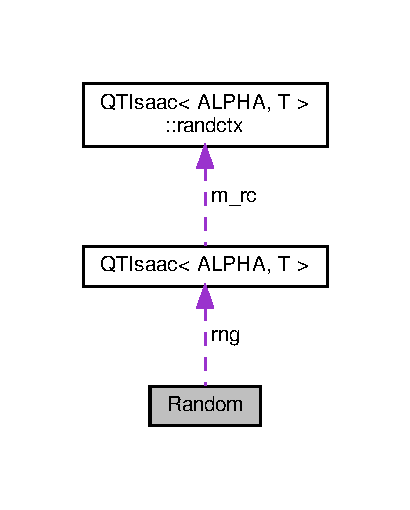
\includegraphics[width=197pt]{classRandom__coll__graph}
\end{center}
\end{figure}
\subsection*{Public Member Functions}
\begin{DoxyCompactItemize}
\item 
N\+T\+L\+::\+ZZ \hyperlink{classRandom_a5347f94bb53028350ad9f46c375aae45}{next\+Big\+Integer} (N\+T\+L\+::\+ZZ \&range)
\item 
N\+T\+L\+::\+ZZ \hyperlink{classRandom_a1d267162c75edb3792dcf29f3125f265}{next\+Big\+Integer} (N\+T\+L\+::\+ZZ \&min, N\+T\+L\+::\+ZZ \&max)
\item 
\hyperlink{classRandom_acb76b49c3903a3c4fb67fd216341f08d}{Random} ()
\item 
\hyperlink{classRandom_a828e4af348ebff33c0785980a4ff4d38}{Random} (Crypto\+P\+P\+::\+Sec\+Byte\+Block \&seed)
\item 
virtual \hyperlink{classRandom_ac0d4eaf1f32df4600eb321cb8dbc0c55}{$\sim$\+Random} ()
\end{DoxyCompactItemize}
\subsection*{Private Attributes}
\begin{DoxyCompactItemize}
\item 
\hyperlink{classQTIsaac}{Q\+T\+Isaac} $\ast$ \hyperlink{classRandom_ac7e446b9b431641c729a6d78ab747781}{rng}
\end{DoxyCompactItemize}


\subsection{Detailed Description}
Implements support for uniformly distributed random arbitrary precision integers. We use the I\+S\+A\+AC cipher as our P\+R\+NG function.

I\+S\+A\+AC has been designed to be cryptographically secure if seeded properly. 

\subsection{Constructor \& Destructor Documentation}
\mbox{\Hypertarget{classRandom_acb76b49c3903a3c4fb67fd216341f08d}\label{classRandom_acb76b49c3903a3c4fb67fd216341f08d}} 
\index{Random@{Random}!Random@{Random}}
\index{Random@{Random}!Random@{Random}}
\subsubsection{\texorpdfstring{Random()}{Random()}\hspace{0.1cm}{\footnotesize\ttfamily [1/2]}}
{\footnotesize\ttfamily Random\+::\+Random (\begin{DoxyParamCaption}{ }\end{DoxyParamCaption})}

Default constructor. Uses device random data to seed the I\+S\+A\+AC cipher. \mbox{\Hypertarget{classRandom_a828e4af348ebff33c0785980a4ff4d38}\label{classRandom_a828e4af348ebff33c0785980a4ff4d38}} 
\index{Random@{Random}!Random@{Random}}
\index{Random@{Random}!Random@{Random}}
\subsubsection{\texorpdfstring{Random()}{Random()}\hspace{0.1cm}{\footnotesize\ttfamily [2/2]}}
{\footnotesize\ttfamily Random\+::\+Random (\begin{DoxyParamCaption}\item[{Crypto\+P\+P\+::\+Sec\+Byte\+Block \&}]{seed }\end{DoxyParamCaption})}

Uses the supplied byte array to seed the I\+S\+A\+AC cipher 
\begin{DoxyParams}{Parameters}
{\em seed} & A byte array \\
\hline
\end{DoxyParams}
\mbox{\Hypertarget{classRandom_ac0d4eaf1f32df4600eb321cb8dbc0c55}\label{classRandom_ac0d4eaf1f32df4600eb321cb8dbc0c55}} 
\index{Random@{Random}!````~Random@{$\sim$\+Random}}
\index{````~Random@{$\sim$\+Random}!Random@{Random}}
\subsubsection{\texorpdfstring{$\sim$\+Random()}{~Random()}}
{\footnotesize\ttfamily Random\+::$\sim$\+Random (\begin{DoxyParamCaption}{ }\end{DoxyParamCaption})\hspace{0.3cm}{\ttfamily [virtual]}}



\subsection{Member Function Documentation}
\mbox{\Hypertarget{classRandom_a5347f94bb53028350ad9f46c375aae45}\label{classRandom_a5347f94bb53028350ad9f46c375aae45}} 
\index{Random@{Random}!next\+Big\+Integer@{next\+Big\+Integer}}
\index{next\+Big\+Integer@{next\+Big\+Integer}!Random@{Random}}
\subsubsection{\texorpdfstring{next\+Big\+Integer()}{nextBigInteger()}\hspace{0.1cm}{\footnotesize\ttfamily [1/2]}}
{\footnotesize\ttfamily N\+T\+L\+::\+ZZ Random\+::next\+Big\+Integer (\begin{DoxyParamCaption}\item[{N\+T\+L\+::\+ZZ \&}]{range }\end{DoxyParamCaption})}

Generate a multiprecision integer in the range 0 to {\ttfamily range-\/1} 
\begin{DoxyParams}{Parameters}
{\em range} & The maximum value of a random integer produced is {\ttfamily range-\/1} \\
\hline
\end{DoxyParams}
\begin{DoxyReturn}{Returns}
A multiprecision integer in the range 0 to {\ttfamily range-\/1} 
\end{DoxyReturn}
Generate a multiprecion integer in the range 0 to {\ttfamily range-\/1} 
\begin{DoxyParams}{Parameters}
{\em range} & The maximum value of a random integer produced is {\ttfamily range-\/1} \\
\hline
\end{DoxyParams}
\begin{DoxyReturn}{Returns}
A multiprecion integer in the range 0 to {\ttfamily range-\/1} 
\end{DoxyReturn}
\mbox{\Hypertarget{classRandom_a1d267162c75edb3792dcf29f3125f265}\label{classRandom_a1d267162c75edb3792dcf29f3125f265}} 
\index{Random@{Random}!next\+Big\+Integer@{next\+Big\+Integer}}
\index{next\+Big\+Integer@{next\+Big\+Integer}!Random@{Random}}
\subsubsection{\texorpdfstring{next\+Big\+Integer()}{nextBigInteger()}\hspace{0.1cm}{\footnotesize\ttfamily [2/2]}}
{\footnotesize\ttfamily N\+T\+L\+::\+ZZ Random\+::next\+Big\+Integer (\begin{DoxyParamCaption}\item[{N\+T\+L\+::\+ZZ \&}]{min,  }\item[{N\+T\+L\+::\+ZZ \&}]{max }\end{DoxyParamCaption})}

Generate a multiprecision integer in the range {\ttfamily min} to {\ttfamily max-\/1} 
\begin{DoxyParams}{Parameters}
{\em min} & The minimum value of a random integer produced \\
\hline
{\em max} & The maximum value of a random integer produced is {\ttfamily max-\/1} \\
\hline
\end{DoxyParams}
\begin{DoxyReturn}{Returns}
A multiprecision integer in the range {\ttfamily min} to {\ttfamily max-\/1} 
\end{DoxyReturn}


\subsection{Member Data Documentation}
\mbox{\Hypertarget{classRandom_ac7e446b9b431641c729a6d78ab747781}\label{classRandom_ac7e446b9b431641c729a6d78ab747781}} 
\index{Random@{Random}!rng@{rng}}
\index{rng@{rng}!Random@{Random}}
\subsubsection{\texorpdfstring{rng}{rng}}
{\footnotesize\ttfamily \hyperlink{classQTIsaac}{Q\+T\+Isaac}$\ast$ Random\+::rng\hspace{0.3cm}{\ttfamily [private]}}

The I\+S\+A\+AC cipher is used to generate P\+R\+Ns. 

The documentation for this class was generated from the following files\+:\begin{DoxyCompactItemize}
\item 
include/\hyperlink{Random_8h}{Random.\+h}\item 
src/\hyperlink{Random_8cpp}{Random.\+cpp}\end{DoxyCompactItemize}

\hypertarget{classSSEDecrypter}{}\section{S\+S\+E\+Decrypter Class Reference}
\label{classSSEDecrypter}\index{S\+S\+E\+Decrypter@{S\+S\+E\+Decrypter}}


{\ttfamily \#include $<$S\+S\+E\+Decrypter.\+h$>$}



Inheritance diagram for S\+S\+E\+Decrypter\+:\nopagebreak
\begin{figure}[H]
\begin{center}
\leavevmode
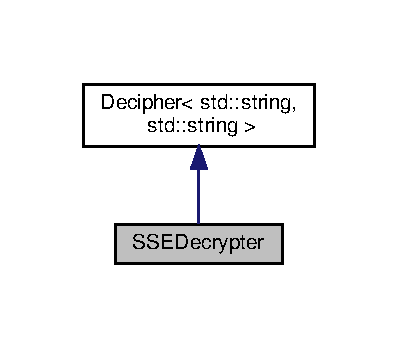
\includegraphics[width=191pt]{classSSEDecrypter__inherit__graph}
\end{center}
\end{figure}


Collaboration diagram for S\+S\+E\+Decrypter\+:\nopagebreak
\begin{figure}[H]
\begin{center}
\leavevmode
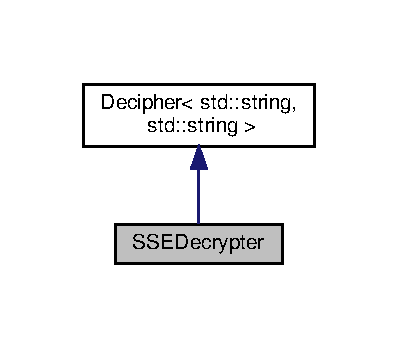
\includegraphics[width=191pt]{classSSEDecrypter__coll__graph}
\end{center}
\end{figure}
\subsection*{Public Member Functions}
\begin{DoxyCompactItemize}
\item 
\hyperlink{classSSEDecrypter_a3ae3f44a17d8b2abb66252d5dee2bf92}{S\+S\+E\+Decrypter} ()
\item 
virtual \hyperlink{classSSEDecrypter_ab99776ce887ce3a992a21def645baf26}{$\sim$\+S\+S\+E\+Decrypter} ()
\item 
void \hyperlink{classSSEDecrypter_a1bdc685b8ea9c5bcc2b29f0c9a3ca7bf}{read\+Secrets\+From\+J\+S\+ON} (std\+::string \&json)
\item 
std\+::string \hyperlink{classSSEDecrypter_afc1522b78aed502f8ca94163fc030ffa}{decrypt} (std\+::string \&ciphertext)
\item 
void \hyperlink{classSSEDecrypter_afb19d398b4862298a831a020d61ffef7}{set\+Key} (Crypto\+P\+P\+::\+Sec\+Byte\+Block \&\hyperlink{classSSEDecrypter_a05c8a6317f2de2cfd37c5474d616d16a}{key})
\item 
void \hyperlink{classSSEDecrypter_a86d8cc2754814cfe59ee69ddf900b1f4}{set\+Key} (std\+::string \&hex\+Encoded\+Key)
\end{DoxyCompactItemize}
\subsection*{Private Member Functions}
\begin{DoxyCompactItemize}
\item 
void \hyperlink{classSSEDecrypter_a4be8d581100ecdbe9a8b75c29f65800c}{decode\+Hex\+String} (std\+::string \&hex\+String, Crypto\+P\+P\+::\+Sec\+Byte\+Block \&bytes)
\end{DoxyCompactItemize}
\subsection*{Private Attributes}
\begin{DoxyCompactItemize}
\item 
Crypto\+P\+P\+::\+Sec\+Byte\+Block \hyperlink{classSSEDecrypter_a05c8a6317f2de2cfd37c5474d616d16a}{key}
\item 
Crypto\+P\+P\+::\+C\+B\+C\+\_\+\+Mode$<$ Crypto\+P\+P\+::\+A\+ES $>$\+::Decryption \hyperlink{classSSEDecrypter_a339c0a434bd2a434b548d9d9e6d6762c}{d}
\end{DoxyCompactItemize}


\subsection{Constructor \& Destructor Documentation}
\mbox{\Hypertarget{classSSEDecrypter_a3ae3f44a17d8b2abb66252d5dee2bf92}\label{classSSEDecrypter_a3ae3f44a17d8b2abb66252d5dee2bf92}} 
\index{S\+S\+E\+Decrypter@{S\+S\+E\+Decrypter}!S\+S\+E\+Decrypter@{S\+S\+E\+Decrypter}}
\index{S\+S\+E\+Decrypter@{S\+S\+E\+Decrypter}!S\+S\+E\+Decrypter@{S\+S\+E\+Decrypter}}
\subsubsection{\texorpdfstring{S\+S\+E\+Decrypter()}{SSEDecrypter()}}
{\footnotesize\ttfamily S\+S\+E\+Decrypter\+::\+S\+S\+E\+Decrypter (\begin{DoxyParamCaption}{ }\end{DoxyParamCaption})}

\mbox{\Hypertarget{classSSEDecrypter_ab99776ce887ce3a992a21def645baf26}\label{classSSEDecrypter_ab99776ce887ce3a992a21def645baf26}} 
\index{S\+S\+E\+Decrypter@{S\+S\+E\+Decrypter}!````~S\+S\+E\+Decrypter@{$\sim$\+S\+S\+E\+Decrypter}}
\index{````~S\+S\+E\+Decrypter@{$\sim$\+S\+S\+E\+Decrypter}!S\+S\+E\+Decrypter@{S\+S\+E\+Decrypter}}
\subsubsection{\texorpdfstring{$\sim$\+S\+S\+E\+Decrypter()}{~SSEDecrypter()}}
{\footnotesize\ttfamily S\+S\+E\+Decrypter\+::$\sim$\+S\+S\+E\+Decrypter (\begin{DoxyParamCaption}{ }\end{DoxyParamCaption})\hspace{0.3cm}{\ttfamily [virtual]}}



\subsection{Member Function Documentation}
\mbox{\Hypertarget{classSSEDecrypter_a4be8d581100ecdbe9a8b75c29f65800c}\label{classSSEDecrypter_a4be8d581100ecdbe9a8b75c29f65800c}} 
\index{S\+S\+E\+Decrypter@{S\+S\+E\+Decrypter}!decode\+Hex\+String@{decode\+Hex\+String}}
\index{decode\+Hex\+String@{decode\+Hex\+String}!S\+S\+E\+Decrypter@{S\+S\+E\+Decrypter}}
\subsubsection{\texorpdfstring{decode\+Hex\+String()}{decodeHexString()}}
{\footnotesize\ttfamily void S\+S\+E\+Decrypter\+::decode\+Hex\+String (\begin{DoxyParamCaption}\item[{std\+::string \&}]{hex\+String,  }\item[{Crypto\+P\+P\+::\+Sec\+Byte\+Block \&}]{bytes }\end{DoxyParamCaption})\hspace{0.3cm}{\ttfamily [private]}}

Decode a hexadecimal string and place the result in {\ttfamily bytes} 
\begin{DoxyParams}{Parameters}
{\em hex\+String} & A hexadecimal string \\
\hline
{\em bytes} & A byte array \\
\hline
\end{DoxyParams}
\mbox{\Hypertarget{classSSEDecrypter_afc1522b78aed502f8ca94163fc030ffa}\label{classSSEDecrypter_afc1522b78aed502f8ca94163fc030ffa}} 
\index{S\+S\+E\+Decrypter@{S\+S\+E\+Decrypter}!decrypt@{decrypt}}
\index{decrypt@{decrypt}!S\+S\+E\+Decrypter@{S\+S\+E\+Decrypter}}
\subsubsection{\texorpdfstring{decrypt()}{decrypt()}}
{\footnotesize\ttfamily std\+::string S\+S\+E\+Decrypter\+::decrypt (\begin{DoxyParamCaption}\item[{std\+::string \&}]{ciphertext }\end{DoxyParamCaption})\hspace{0.3cm}{\ttfamily [virtual]}}

Decrypts a ciphertext 
\begin{DoxyParams}{Parameters}
{\em ciphertext} & Ciphertext value \\
\hline
\end{DoxyParams}
\begin{DoxyReturn}{Returns}
Plaintext value 
\end{DoxyReturn}


Implements \hyperlink{classDecipher_ac6b8c369eda2d7e17fa90cb594cf41b6}{Decipher$<$ std\+::string, std\+::string $>$}.

\mbox{\Hypertarget{classSSEDecrypter_a1bdc685b8ea9c5bcc2b29f0c9a3ca7bf}\label{classSSEDecrypter_a1bdc685b8ea9c5bcc2b29f0c9a3ca7bf}} 
\index{S\+S\+E\+Decrypter@{S\+S\+E\+Decrypter}!read\+Secrets\+From\+J\+S\+ON@{read\+Secrets\+From\+J\+S\+ON}}
\index{read\+Secrets\+From\+J\+S\+ON@{read\+Secrets\+From\+J\+S\+ON}!S\+S\+E\+Decrypter@{S\+S\+E\+Decrypter}}
\subsubsection{\texorpdfstring{read\+Secrets\+From\+J\+S\+O\+N()}{readSecretsFromJSON()}}
{\footnotesize\ttfamily void S\+S\+E\+Decrypter\+::read\+Secrets\+From\+J\+S\+ON (\begin{DoxyParamCaption}\item[{std\+::string \&}]{string }\end{DoxyParamCaption})\hspace{0.3cm}{\ttfamily [virtual]}}

Reads the cipher secrets in from a J\+S\+ON string 
\begin{DoxyParams}{Parameters}
{\em string} & J\+S\+ON string \\
\hline
\end{DoxyParams}


Implements \hyperlink{classDecipher_a39aea002012130201e12a8fa7d84dda5}{Decipher$<$ std\+::string, std\+::string $>$}.

\mbox{\Hypertarget{classSSEDecrypter_afb19d398b4862298a831a020d61ffef7}\label{classSSEDecrypter_afb19d398b4862298a831a020d61ffef7}} 
\index{S\+S\+E\+Decrypter@{S\+S\+E\+Decrypter}!set\+Key@{set\+Key}}
\index{set\+Key@{set\+Key}!S\+S\+E\+Decrypter@{S\+S\+E\+Decrypter}}
\subsubsection{\texorpdfstring{set\+Key()}{setKey()}\hspace{0.1cm}{\footnotesize\ttfamily [1/2]}}
{\footnotesize\ttfamily void S\+S\+E\+Decrypter\+::set\+Key (\begin{DoxyParamCaption}\item[{Crypto\+P\+P\+::\+Sec\+Byte\+Block \&}]{key }\end{DoxyParamCaption})}

Set they cipher key 
\begin{DoxyParams}{Parameters}
{\em key} & Byte array \\
\hline
\end{DoxyParams}
\mbox{\Hypertarget{classSSEDecrypter_a86d8cc2754814cfe59ee69ddf900b1f4}\label{classSSEDecrypter_a86d8cc2754814cfe59ee69ddf900b1f4}} 
\index{S\+S\+E\+Decrypter@{S\+S\+E\+Decrypter}!set\+Key@{set\+Key}}
\index{set\+Key@{set\+Key}!S\+S\+E\+Decrypter@{S\+S\+E\+Decrypter}}
\subsubsection{\texorpdfstring{set\+Key()}{setKey()}\hspace{0.1cm}{\footnotesize\ttfamily [2/2]}}
{\footnotesize\ttfamily void S\+S\+E\+Decrypter\+::set\+Key (\begin{DoxyParamCaption}\item[{std\+::string \&}]{hex\+Encoded\+Key }\end{DoxyParamCaption})}

Set the cipher key 
\begin{DoxyParams}{Parameters}
{\em hex\+Encoded\+Key} & Hexadecimal encoded string \\
\hline
\end{DoxyParams}


\subsection{Member Data Documentation}
\mbox{\Hypertarget{classSSEDecrypter_a339c0a434bd2a434b548d9d9e6d6762c}\label{classSSEDecrypter_a339c0a434bd2a434b548d9d9e6d6762c}} 
\index{S\+S\+E\+Decrypter@{S\+S\+E\+Decrypter}!d@{d}}
\index{d@{d}!S\+S\+E\+Decrypter@{S\+S\+E\+Decrypter}}
\subsubsection{\texorpdfstring{d}{d}}
{\footnotesize\ttfamily Crypto\+P\+P\+::\+C\+B\+C\+\_\+\+Mode$<$Crypto\+P\+P\+::\+A\+ES$>$\+::Decryption S\+S\+E\+Decrypter\+::d\hspace{0.3cm}{\ttfamily [private]}}

The decryption cipher (A\+ES in C\+BC mode) \mbox{\Hypertarget{classSSEDecrypter_a05c8a6317f2de2cfd37c5474d616d16a}\label{classSSEDecrypter_a05c8a6317f2de2cfd37c5474d616d16a}} 
\index{S\+S\+E\+Decrypter@{S\+S\+E\+Decrypter}!key@{key}}
\index{key@{key}!S\+S\+E\+Decrypter@{S\+S\+E\+Decrypter}}
\subsubsection{\texorpdfstring{key}{key}}
{\footnotesize\ttfamily Crypto\+P\+P\+::\+Sec\+Byte\+Block S\+S\+E\+Decrypter\+::key\hspace{0.3cm}{\ttfamily [private]}}

The cipher key 

The documentation for this class was generated from the following files\+:\begin{DoxyCompactItemize}
\item 
include/\hyperlink{SSEDecrypter_8h}{S\+S\+E\+Decrypter.\+h}\item 
src/\hyperlink{SSEDecrypter_8cpp}{S\+S\+E\+Decrypter.\+cpp}\end{DoxyCompactItemize}

\hypertarget{classSSEEncrypter}{}\section{S\+S\+E\+Encrypter Class Reference}
\label{classSSEEncrypter}\index{S\+S\+E\+Encrypter@{S\+S\+E\+Encrypter}}


{\ttfamily \#include $<$S\+S\+E\+Encrypter.\+h$>$}



Inheritance diagram for S\+S\+E\+Encrypter\+:\nopagebreak
\begin{figure}[H]
\begin{center}
\leavevmode
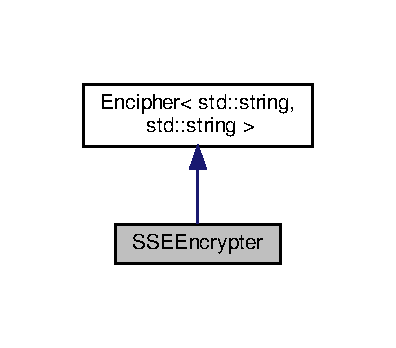
\includegraphics[width=190pt]{classSSEEncrypter__inherit__graph}
\end{center}
\end{figure}


Collaboration diagram for S\+S\+E\+Encrypter\+:\nopagebreak
\begin{figure}[H]
\begin{center}
\leavevmode
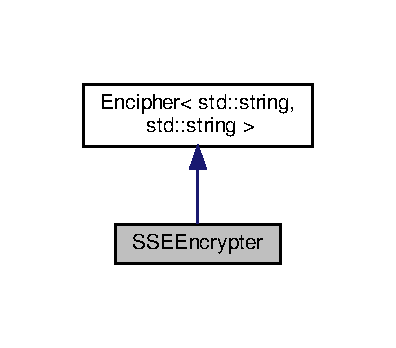
\includegraphics[width=190pt]{classSSEEncrypter__coll__graph}
\end{center}
\end{figure}
\subsection*{Public Member Functions}
\begin{DoxyCompactItemize}
\item 
std\+::string \hyperlink{classSSEEncrypter_ab13571d2a7a8875226bf8901cd080949}{encrypt} (std\+::string \&plaintext) override
\item 
Crypto\+P\+P\+::\+Sec\+Byte\+Block \hyperlink{classSSEEncrypter_ae9562054f00a5f9899b019568cad2338}{get\+Key} ()
\item 
Crypto\+P\+P\+::\+Sec\+Byte\+Block \hyperlink{classSSEEncrypter_a0fa90c40369bc916f61e870fd39a42c2}{get\+Key\+Gen\+Key} ()
\item 
std\+::string \hyperlink{classSSEEncrypter_a741ba1ef98a1f1b294ed3904738cd888}{get\+Hex\+Encoded\+Key} ()
\item 
std\+::string \hyperlink{classSSEEncrypter_abaefa48cff26cad49a17a1bd2586dbc7}{get\+Hex\+Encoded\+Key\+Gen\+Key} ()
\item 
Crypto\+P\+P\+::\+Sec\+Byte\+Block \hyperlink{classSSEEncrypter_ae81cc103149e1db15c577c8b474f9217}{create\+Search\+Key} (std\+::string \&word)
\item 
std\+::string \hyperlink{classSSEEncrypter_a09dac9d519550e0375f0f677aab69bfb}{create\+Hex\+Encoded\+Search\+Key} (std\+::string \&word)
\item 
std\+::string \hyperlink{classSSEEncrypter_a70e01b58fe0de0931cdb00ee97ee4af9}{write\+Secrets\+To\+J\+S\+ON} () override
\item 
\hyperlink{classSSEEncrypter_a4b45442fa1025d82ed499241da4796bf}{S\+S\+E\+Encrypter} ()
\item 
\hyperlink{classSSEEncrypter_ae109735e8bf9f5a32d6f481e6d208bd8}{S\+S\+E\+Encrypter} (std\+::string \&secrets)
\item 
virtual \hyperlink{classSSEEncrypter_a249d1527f2d370c693534c3d435a522a}{$\sim$\+S\+S\+E\+Encrypter} ()
\end{DoxyCompactItemize}
\subsection*{Private Member Functions}
\begin{DoxyCompactItemize}
\item 
void \hyperlink{classSSEEncrypter_a668394973e3f574ca24588c5a0763f5f}{decode\+Hex\+String} (std\+::string \&hex\+String, Crypto\+P\+P\+::\+Sec\+Byte\+Block \&bytes)
\end{DoxyCompactItemize}
\subsection*{Private Attributes}
\begin{DoxyCompactItemize}
\item 
Crypto\+P\+P\+::\+Sec\+Byte\+Block \hyperlink{classSSEEncrypter_a35dbd89d8820118bf71d6cd483e64ac8}{key\+Gen\+Key}
\item 
Crypto\+P\+P\+::\+Sec\+Byte\+Block \hyperlink{classSSEEncrypter_ab6fb0b44e024a40077fd44672ad78f28}{key\+Gen\+IV}
\item 
Crypto\+P\+P\+::\+Sec\+Byte\+Block \hyperlink{classSSEEncrypter_afc4ceb0c421614857c18b152a976c29a}{key}
\item 
Crypto\+P\+P\+::\+C\+B\+C\+\_\+\+Mode$<$ Crypto\+P\+P\+::\+A\+ES $>$\+::Encryption \hyperlink{classSSEEncrypter_a2831d301099a3d5548479996e3c8cf4b}{e}
\item 
Crypto\+P\+P\+::\+C\+B\+C\+\_\+\+Mode$<$ Crypto\+P\+P\+::\+A\+ES $>$\+::Encryption \hyperlink{classSSEEncrypter_a43d9006f3db0d57fa02069977946335b}{keygen}
\item 
Crypto\+P\+P\+::\+C\+M\+AC$<$ Crypto\+P\+P\+::\+A\+ES $>$ \hyperlink{classSSEEncrypter_a67939726bb84cb761535642873c3b10c}{mac}
\end{DoxyCompactItemize}


\subsection{Constructor \& Destructor Documentation}
\mbox{\Hypertarget{classSSEEncrypter_a4b45442fa1025d82ed499241da4796bf}\label{classSSEEncrypter_a4b45442fa1025d82ed499241da4796bf}} 
\index{S\+S\+E\+Encrypter@{S\+S\+E\+Encrypter}!S\+S\+E\+Encrypter@{S\+S\+E\+Encrypter}}
\index{S\+S\+E\+Encrypter@{S\+S\+E\+Encrypter}!S\+S\+E\+Encrypter@{S\+S\+E\+Encrypter}}
\subsubsection{\texorpdfstring{S\+S\+E\+Encrypter()}{SSEEncrypter()}\hspace{0.1cm}{\footnotesize\ttfamily [1/2]}}
{\footnotesize\ttfamily S\+S\+E\+Encrypter\+::\+S\+S\+E\+Encrypter (\begin{DoxyParamCaption}{ }\end{DoxyParamCaption})}

The constructor generates three random values\+: a 256-\/bit cipher key; a 256-\/bit key for the key generation cipher; and an initialisation vector for the key generation cipher. \mbox{\Hypertarget{classSSEEncrypter_ae109735e8bf9f5a32d6f481e6d208bd8}\label{classSSEEncrypter_ae109735e8bf9f5a32d6f481e6d208bd8}} 
\index{S\+S\+E\+Encrypter@{S\+S\+E\+Encrypter}!S\+S\+E\+Encrypter@{S\+S\+E\+Encrypter}}
\index{S\+S\+E\+Encrypter@{S\+S\+E\+Encrypter}!S\+S\+E\+Encrypter@{S\+S\+E\+Encrypter}}
\subsubsection{\texorpdfstring{S\+S\+E\+Encrypter()}{SSEEncrypter()}\hspace{0.1cm}{\footnotesize\ttfamily [2/2]}}
{\footnotesize\ttfamily S\+S\+E\+Encrypter\+::\+S\+S\+E\+Encrypter (\begin{DoxyParamCaption}\item[{std\+::string \&}]{secrets }\end{DoxyParamCaption})}

Initialises the cipher using pre-\/existing secrets in the supplied J\+S\+ON string 
\begin{DoxyParams}{Parameters}
{\em secrets} & A J\+S\+ON string containing the hex encoded cipher keys \\
\hline
\end{DoxyParams}
\mbox{\Hypertarget{classSSEEncrypter_a249d1527f2d370c693534c3d435a522a}\label{classSSEEncrypter_a249d1527f2d370c693534c3d435a522a}} 
\index{S\+S\+E\+Encrypter@{S\+S\+E\+Encrypter}!````~S\+S\+E\+Encrypter@{$\sim$\+S\+S\+E\+Encrypter}}
\index{````~S\+S\+E\+Encrypter@{$\sim$\+S\+S\+E\+Encrypter}!S\+S\+E\+Encrypter@{S\+S\+E\+Encrypter}}
\subsubsection{\texorpdfstring{$\sim$\+S\+S\+E\+Encrypter()}{~SSEEncrypter()}}
{\footnotesize\ttfamily S\+S\+E\+Encrypter\+::$\sim$\+S\+S\+E\+Encrypter (\begin{DoxyParamCaption}{ }\end{DoxyParamCaption})\hspace{0.3cm}{\ttfamily [virtual]}}



\subsection{Member Function Documentation}
\mbox{\Hypertarget{classSSEEncrypter_a09dac9d519550e0375f0f677aab69bfb}\label{classSSEEncrypter_a09dac9d519550e0375f0f677aab69bfb}} 
\index{S\+S\+E\+Encrypter@{S\+S\+E\+Encrypter}!create\+Hex\+Encoded\+Search\+Key@{create\+Hex\+Encoded\+Search\+Key}}
\index{create\+Hex\+Encoded\+Search\+Key@{create\+Hex\+Encoded\+Search\+Key}!S\+S\+E\+Encrypter@{S\+S\+E\+Encrypter}}
\subsubsection{\texorpdfstring{create\+Hex\+Encoded\+Search\+Key()}{createHexEncodedSearchKey()}}
{\footnotesize\ttfamily std\+::string S\+S\+E\+Encrypter\+::create\+Hex\+Encoded\+Search\+Key (\begin{DoxyParamCaption}\item[{std\+::string \&}]{word }\end{DoxyParamCaption})}

Convenience method to generate and hexadecimal encode the search key 
\begin{DoxyParams}{Parameters}
{\em word} & Input word \\
\hline
\end{DoxyParams}
\begin{DoxyReturn}{Returns}
A hexadecimal encoded string 
\end{DoxyReturn}
\mbox{\Hypertarget{classSSEEncrypter_ae81cc103149e1db15c577c8b474f9217}\label{classSSEEncrypter_ae81cc103149e1db15c577c8b474f9217}} 
\index{S\+S\+E\+Encrypter@{S\+S\+E\+Encrypter}!create\+Search\+Key@{create\+Search\+Key}}
\index{create\+Search\+Key@{create\+Search\+Key}!S\+S\+E\+Encrypter@{S\+S\+E\+Encrypter}}
\subsubsection{\texorpdfstring{create\+Search\+Key()}{createSearchKey()}}
{\footnotesize\ttfamily Crypto\+P\+P\+::\+Sec\+Byte\+Block S\+S\+E\+Encrypter\+::create\+Search\+Key (\begin{DoxyParamCaption}\item[{std\+::string \&}]{word }\end{DoxyParamCaption})}

This function generates a M\+AC key using a deterministic cipher (A\+ES with a constant initialisation vector). This is applied to the input word 
\begin{DoxyParams}{Parameters}
{\em word} & Input word \\
\hline
\end{DoxyParams}
\begin{DoxyReturn}{Returns}
A 16 or 32 byte array 
\end{DoxyReturn}
\mbox{\Hypertarget{classSSEEncrypter_a668394973e3f574ca24588c5a0763f5f}\label{classSSEEncrypter_a668394973e3f574ca24588c5a0763f5f}} 
\index{S\+S\+E\+Encrypter@{S\+S\+E\+Encrypter}!decode\+Hex\+String@{decode\+Hex\+String}}
\index{decode\+Hex\+String@{decode\+Hex\+String}!S\+S\+E\+Encrypter@{S\+S\+E\+Encrypter}}
\subsubsection{\texorpdfstring{decode\+Hex\+String()}{decodeHexString()}}
{\footnotesize\ttfamily void S\+S\+E\+Encrypter\+::decode\+Hex\+String (\begin{DoxyParamCaption}\item[{std\+::string \&}]{hex\+String,  }\item[{Crypto\+P\+P\+::\+Sec\+Byte\+Block \&}]{bytes }\end{DoxyParamCaption})\hspace{0.3cm}{\ttfamily [private]}}

Decode a hexadecimal string to a byte array 
\begin{DoxyParams}{Parameters}
{\em hex\+String} & Hexadecimal string \\
\hline
{\em bytes} & Byte array \\
\hline
\end{DoxyParams}
\mbox{\Hypertarget{classSSEEncrypter_ab13571d2a7a8875226bf8901cd080949}\label{classSSEEncrypter_ab13571d2a7a8875226bf8901cd080949}} 
\index{S\+S\+E\+Encrypter@{S\+S\+E\+Encrypter}!encrypt@{encrypt}}
\index{encrypt@{encrypt}!S\+S\+E\+Encrypter@{S\+S\+E\+Encrypter}}
\subsubsection{\texorpdfstring{encrypt()}{encrypt()}}
{\footnotesize\ttfamily std\+::string S\+S\+E\+Encrypter\+::encrypt (\begin{DoxyParamCaption}\item[{std\+::string \&}]{plaintext }\end{DoxyParamCaption})\hspace{0.3cm}{\ttfamily [override]}, {\ttfamily [virtual]}}

Encrypts the plaintext word as a triple of a 16-\/byte intialisation vector, an A\+ES ciphertext, and a M\+AC tag. Currently, this triple is implmented as a hex encoded J\+S\+ON object for convenience. However, it could easily be altered to return a C++ tuple or a concatenated byte sequence. 
\begin{DoxyParams}{Parameters}
{\em plaintext} & A string \\
\hline
\end{DoxyParams}
\begin{DoxyReturn}{Returns}
A J\+S\+ON object 
\end{DoxyReturn}


Implements \hyperlink{classEncipher_aaf8138eb280608bfd03c6eb762ffc010}{Encipher$<$ std\+::string, std\+::string $>$}.

\mbox{\Hypertarget{classSSEEncrypter_a741ba1ef98a1f1b294ed3904738cd888}\label{classSSEEncrypter_a741ba1ef98a1f1b294ed3904738cd888}} 
\index{S\+S\+E\+Encrypter@{S\+S\+E\+Encrypter}!get\+Hex\+Encoded\+Key@{get\+Hex\+Encoded\+Key}}
\index{get\+Hex\+Encoded\+Key@{get\+Hex\+Encoded\+Key}!S\+S\+E\+Encrypter@{S\+S\+E\+Encrypter}}
\subsubsection{\texorpdfstring{get\+Hex\+Encoded\+Key()}{getHexEncodedKey()}}
{\footnotesize\ttfamily std\+::string S\+S\+E\+Encrypter\+::get\+Hex\+Encoded\+Key (\begin{DoxyParamCaption}{ }\end{DoxyParamCaption})}

Convenience method to get the key as a hexadecimal encoded string. \begin{DoxyReturn}{Returns}
hexadecimal encoded string 
\end{DoxyReturn}
\mbox{\Hypertarget{classSSEEncrypter_abaefa48cff26cad49a17a1bd2586dbc7}\label{classSSEEncrypter_abaefa48cff26cad49a17a1bd2586dbc7}} 
\index{S\+S\+E\+Encrypter@{S\+S\+E\+Encrypter}!get\+Hex\+Encoded\+Key\+Gen\+Key@{get\+Hex\+Encoded\+Key\+Gen\+Key}}
\index{get\+Hex\+Encoded\+Key\+Gen\+Key@{get\+Hex\+Encoded\+Key\+Gen\+Key}!S\+S\+E\+Encrypter@{S\+S\+E\+Encrypter}}
\subsubsection{\texorpdfstring{get\+Hex\+Encoded\+Key\+Gen\+Key()}{getHexEncodedKeyGenKey()}}
{\footnotesize\ttfamily std\+::string S\+S\+E\+Encrypter\+::get\+Hex\+Encoded\+Key\+Gen\+Key (\begin{DoxyParamCaption}{ }\end{DoxyParamCaption})}

Convenience method to get the key as a hexadecimal encoded string. \begin{DoxyReturn}{Returns}
hexadecimal encoded string 
\end{DoxyReturn}
\mbox{\Hypertarget{classSSEEncrypter_ae9562054f00a5f9899b019568cad2338}\label{classSSEEncrypter_ae9562054f00a5f9899b019568cad2338}} 
\index{S\+S\+E\+Encrypter@{S\+S\+E\+Encrypter}!get\+Key@{get\+Key}}
\index{get\+Key@{get\+Key}!S\+S\+E\+Encrypter@{S\+S\+E\+Encrypter}}
\subsubsection{\texorpdfstring{get\+Key()}{getKey()}}
{\footnotesize\ttfamily Crypto\+P\+P\+::\+Sec\+Byte\+Block S\+S\+E\+Encrypter\+::get\+Key (\begin{DoxyParamCaption}{ }\end{DoxyParamCaption})}

Accessor to return the A\+ES cipher key \begin{DoxyReturn}{Returns}
Key byte sequence 
\end{DoxyReturn}
\mbox{\Hypertarget{classSSEEncrypter_a0fa90c40369bc916f61e870fd39a42c2}\label{classSSEEncrypter_a0fa90c40369bc916f61e870fd39a42c2}} 
\index{S\+S\+E\+Encrypter@{S\+S\+E\+Encrypter}!get\+Key\+Gen\+Key@{get\+Key\+Gen\+Key}}
\index{get\+Key\+Gen\+Key@{get\+Key\+Gen\+Key}!S\+S\+E\+Encrypter@{S\+S\+E\+Encrypter}}
\subsubsection{\texorpdfstring{get\+Key\+Gen\+Key()}{getKeyGenKey()}}
{\footnotesize\ttfamily Crypto\+P\+P\+::\+Sec\+Byte\+Block S\+S\+E\+Encrypter\+::get\+Key\+Gen\+Key (\begin{DoxyParamCaption}{ }\end{DoxyParamCaption})}

Accessor to return the key for the deterministic A\+ES instance used for key generation \begin{DoxyReturn}{Returns}
Key byte sequence 
\end{DoxyReturn}
\mbox{\Hypertarget{classSSEEncrypter_a70e01b58fe0de0931cdb00ee97ee4af9}\label{classSSEEncrypter_a70e01b58fe0de0931cdb00ee97ee4af9}} 
\index{S\+S\+E\+Encrypter@{S\+S\+E\+Encrypter}!write\+Secrets\+To\+J\+S\+ON@{write\+Secrets\+To\+J\+S\+ON}}
\index{write\+Secrets\+To\+J\+S\+ON@{write\+Secrets\+To\+J\+S\+ON}!S\+S\+E\+Encrypter@{S\+S\+E\+Encrypter}}
\subsubsection{\texorpdfstring{write\+Secrets\+To\+J\+S\+O\+N()}{writeSecretsToJSON()}}
{\footnotesize\ttfamily std\+::string S\+S\+E\+Encrypter\+::write\+Secrets\+To\+J\+S\+ON (\begin{DoxyParamCaption}{ }\end{DoxyParamCaption})\hspace{0.3cm}{\ttfamily [override]}, {\ttfamily [virtual]}}

Writes cipher secrets out to a J\+S\+ON string \begin{DoxyReturn}{Returns}
J\+S\+ON string 
\end{DoxyReturn}


Implements \hyperlink{classEncipher_a27d3efa1e364c1f0d7def65454c61b85}{Encipher$<$ std\+::string, std\+::string $>$}.



\subsection{Member Data Documentation}
\mbox{\Hypertarget{classSSEEncrypter_a2831d301099a3d5548479996e3c8cf4b}\label{classSSEEncrypter_a2831d301099a3d5548479996e3c8cf4b}} 
\index{S\+S\+E\+Encrypter@{S\+S\+E\+Encrypter}!e@{e}}
\index{e@{e}!S\+S\+E\+Encrypter@{S\+S\+E\+Encrypter}}
\subsubsection{\texorpdfstring{e}{e}}
{\footnotesize\ttfamily Crypto\+P\+P\+::\+C\+B\+C\+\_\+\+Mode$<$Crypto\+P\+P\+::\+A\+ES$>$\+::Encryption S\+S\+E\+Encrypter\+::e\hspace{0.3cm}{\ttfamily [private]}}

The encryption cipher. A\+ES is C\+BC mode. \mbox{\Hypertarget{classSSEEncrypter_afc4ceb0c421614857c18b152a976c29a}\label{classSSEEncrypter_afc4ceb0c421614857c18b152a976c29a}} 
\index{S\+S\+E\+Encrypter@{S\+S\+E\+Encrypter}!key@{key}}
\index{key@{key}!S\+S\+E\+Encrypter@{S\+S\+E\+Encrypter}}
\subsubsection{\texorpdfstring{key}{key}}
{\footnotesize\ttfamily Crypto\+P\+P\+::\+Sec\+Byte\+Block S\+S\+E\+Encrypter\+::key\hspace{0.3cm}{\ttfamily [private]}}

The 256-\/bit key for the encryption cipher \mbox{\Hypertarget{classSSEEncrypter_a43d9006f3db0d57fa02069977946335b}\label{classSSEEncrypter_a43d9006f3db0d57fa02069977946335b}} 
\index{S\+S\+E\+Encrypter@{S\+S\+E\+Encrypter}!keygen@{keygen}}
\index{keygen@{keygen}!S\+S\+E\+Encrypter@{S\+S\+E\+Encrypter}}
\subsubsection{\texorpdfstring{keygen}{keygen}}
{\footnotesize\ttfamily Crypto\+P\+P\+::\+C\+B\+C\+\_\+\+Mode$<$Crypto\+P\+P\+::\+A\+ES$>$\+::Encryption S\+S\+E\+Encrypter\+::keygen\hspace{0.3cm}{\ttfamily [private]}}

The key generation cipher. A\+ES is C\+BC mode. \mbox{\Hypertarget{classSSEEncrypter_ab6fb0b44e024a40077fd44672ad78f28}\label{classSSEEncrypter_ab6fb0b44e024a40077fd44672ad78f28}} 
\index{S\+S\+E\+Encrypter@{S\+S\+E\+Encrypter}!key\+Gen\+IV@{key\+Gen\+IV}}
\index{key\+Gen\+IV@{key\+Gen\+IV}!S\+S\+E\+Encrypter@{S\+S\+E\+Encrypter}}
\subsubsection{\texorpdfstring{key\+Gen\+IV}{keyGenIV}}
{\footnotesize\ttfamily Crypto\+P\+P\+::\+Sec\+Byte\+Block S\+S\+E\+Encrypter\+::key\+Gen\+IV\hspace{0.3cm}{\ttfamily [private]}}

The initialization vector for the key generation cipher \mbox{\Hypertarget{classSSEEncrypter_a35dbd89d8820118bf71d6cd483e64ac8}\label{classSSEEncrypter_a35dbd89d8820118bf71d6cd483e64ac8}} 
\index{S\+S\+E\+Encrypter@{S\+S\+E\+Encrypter}!key\+Gen\+Key@{key\+Gen\+Key}}
\index{key\+Gen\+Key@{key\+Gen\+Key}!S\+S\+E\+Encrypter@{S\+S\+E\+Encrypter}}
\subsubsection{\texorpdfstring{key\+Gen\+Key}{keyGenKey}}
{\footnotesize\ttfamily Crypto\+P\+P\+::\+Sec\+Byte\+Block S\+S\+E\+Encrypter\+::key\+Gen\+Key\hspace{0.3cm}{\ttfamily [private]}}

The 256-\/bit key for the key generation cipher \mbox{\Hypertarget{classSSEEncrypter_a67939726bb84cb761535642873c3b10c}\label{classSSEEncrypter_a67939726bb84cb761535642873c3b10c}} 
\index{S\+S\+E\+Encrypter@{S\+S\+E\+Encrypter}!mac@{mac}}
\index{mac@{mac}!S\+S\+E\+Encrypter@{S\+S\+E\+Encrypter}}
\subsubsection{\texorpdfstring{mac}{mac}}
{\footnotesize\ttfamily Crypto\+P\+P\+::\+C\+M\+AC$<$Crypto\+P\+P\+::\+A\+ES$>$ S\+S\+E\+Encrypter\+::mac\hspace{0.3cm}{\ttfamily [private]}}

The M\+AC algorithm. 

The documentation for this class was generated from the following files\+:\begin{DoxyCompactItemize}
\item 
include/\hyperlink{SSEEncrypter_8h}{S\+S\+E\+Encrypter.\+h}\item 
src/\hyperlink{SSEEncrypter_8cpp}{S\+S\+E\+Encrypter.\+cpp}\end{DoxyCompactItemize}

\chapter{File Documentation}
\hypertarget{Decipher_8hpp}{}\section{include/\+Decipher.hpp File Reference}
\label{Decipher_8hpp}\index{include/\+Decipher.\+hpp@{include/\+Decipher.\+hpp}}
{\ttfamily \#include $<$string$>$}\newline
Include dependency graph for Decipher.\+hpp\+:
\nopagebreak
\begin{figure}[H]
\begin{center}
\leavevmode
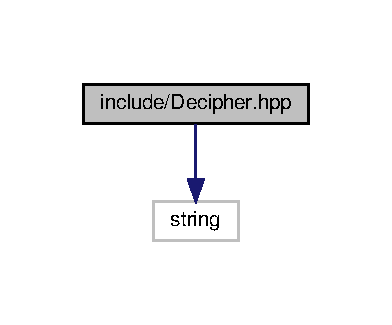
\includegraphics[width=188pt]{Decipher_8hpp__incl}
\end{center}
\end{figure}
This graph shows which files directly or indirectly include this file\+:
\nopagebreak
\begin{figure}[H]
\begin{center}
\leavevmode
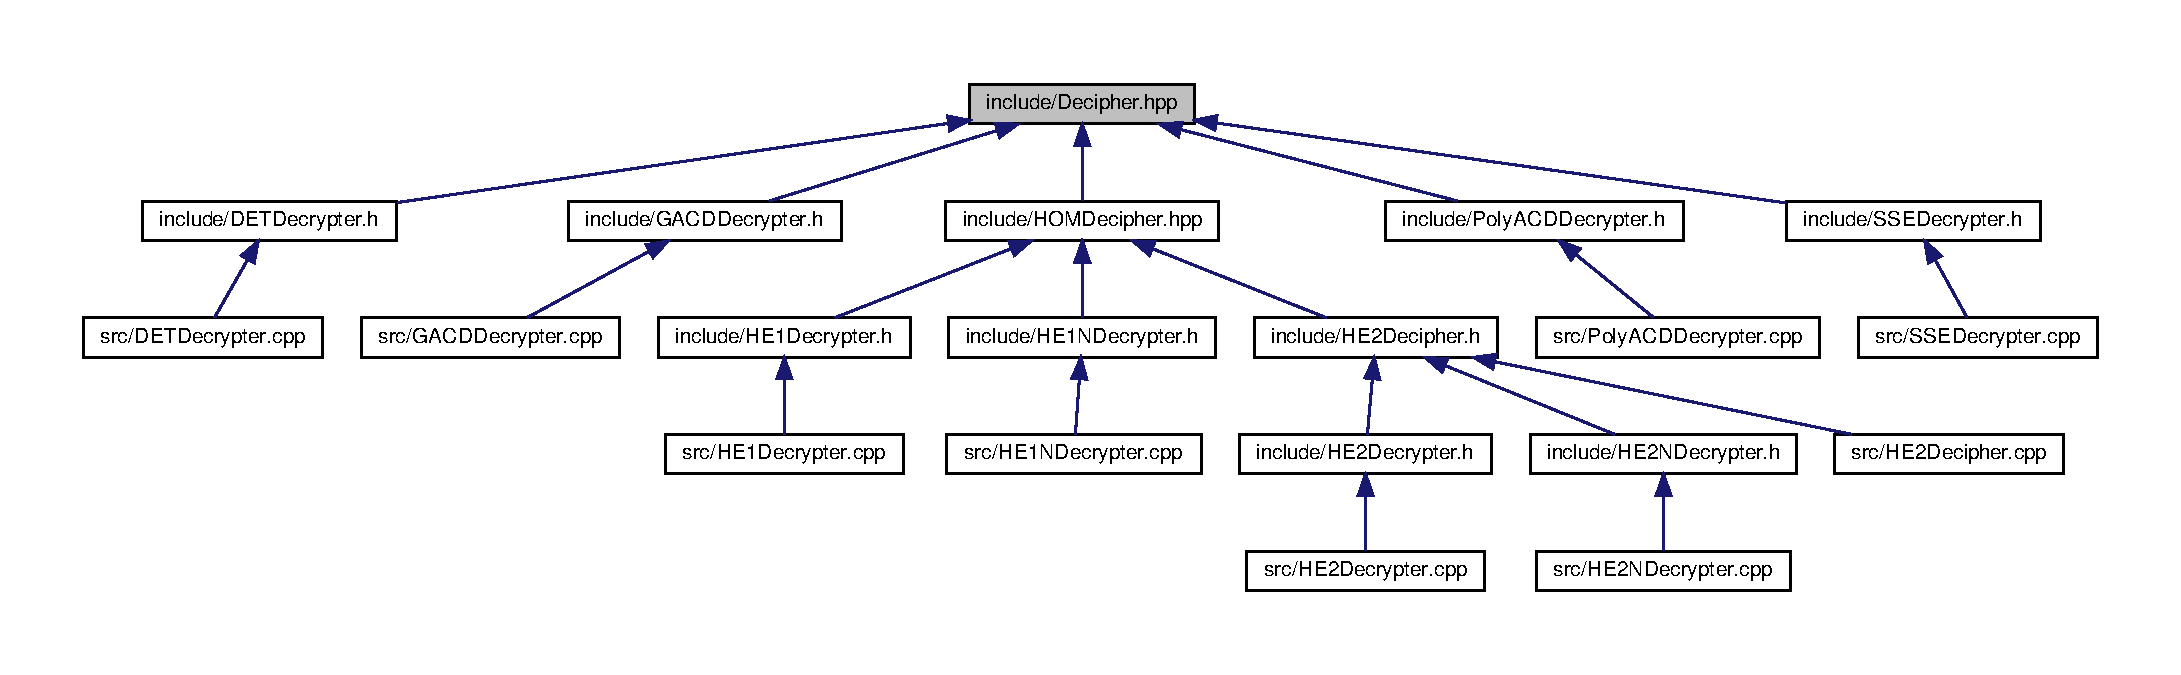
\includegraphics[width=350pt]{Decipher_8hpp__dep__incl}
\end{center}
\end{figure}
\subsection*{Classes}
\begin{DoxyCompactItemize}
\item 
class \hyperlink{classDecipher}{Decipher$<$ C, P $>$}
\end{DoxyCompactItemize}

\hypertarget{DETDecrypter_8h}{}\section{include/\+D\+E\+T\+Decrypter.h File Reference}
\label{DETDecrypter_8h}\index{include/\+D\+E\+T\+Decrypter.\+h@{include/\+D\+E\+T\+Decrypter.\+h}}
{\ttfamily \#include $<$string$>$}\newline
{\ttfamily \#include $<$vector$>$}\newline
{\ttfamily \#include $<$cryptopp/cryptlib.\+h$>$}\newline
{\ttfamily \#include $<$cryptopp/aes.\+h$>$}\newline
{\ttfamily \#include $<$cryptopp/ccm.\+h$>$}\newline
{\ttfamily \#include $<$cryptopp/secblock.\+h$>$}\newline
{\ttfamily \#include \char`\"{}Decipher.\+hpp\char`\"{}}\newline
Include dependency graph for D\+E\+T\+Decrypter.\+h\+:
\nopagebreak
\begin{figure}[H]
\begin{center}
\leavevmode
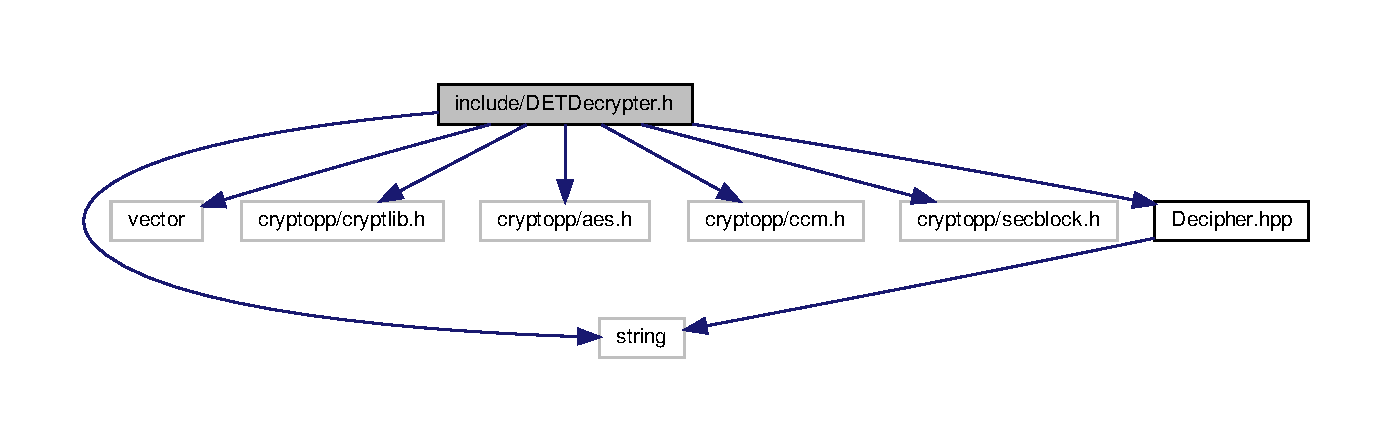
\includegraphics[width=350pt]{DETDecrypter_8h__incl}
\end{center}
\end{figure}
This graph shows which files directly or indirectly include this file\+:
\nopagebreak
\begin{figure}[H]
\begin{center}
\leavevmode
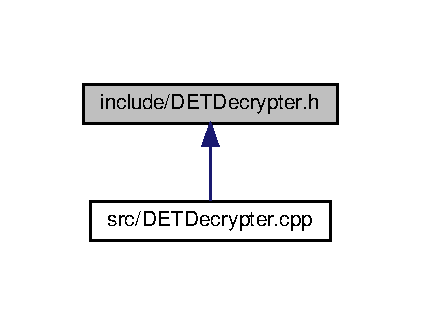
\includegraphics[width=202pt]{DETDecrypter_8h__dep__incl}
\end{center}
\end{figure}
\subsection*{Classes}
\begin{DoxyCompactItemize}
\item 
class \hyperlink{classDETDecrypter}{D\+E\+T\+Decrypter}
\end{DoxyCompactItemize}

\hypertarget{DETEncrypter_8h}{}\section{include/\+D\+E\+T\+Encrypter.h File Reference}
\label{DETEncrypter_8h}\index{include/\+D\+E\+T\+Encrypter.\+h@{include/\+D\+E\+T\+Encrypter.\+h}}
{\ttfamily \#include $<$string$>$}\newline
{\ttfamily \#include $<$vector$>$}\newline
{\ttfamily \#include $<$cryptopp/cryptlib.\+h$>$}\newline
{\ttfamily \#include $<$cryptopp/aes.\+h$>$}\newline
{\ttfamily \#include $<$cryptopp/ccm.\+h$>$}\newline
{\ttfamily \#include $<$cryptopp/secblock.\+h$>$}\newline
{\ttfamily \#include \char`\"{}Encipher.\+hpp\char`\"{}}\newline
Include dependency graph for D\+E\+T\+Encrypter.\+h\+:
\nopagebreak
\begin{figure}[H]
\begin{center}
\leavevmode
\includegraphics[width=350pt]{DETEncrypter_8h__incl}
\end{center}
\end{figure}
This graph shows which files directly or indirectly include this file\+:
\nopagebreak
\begin{figure}[H]
\begin{center}
\leavevmode
\includegraphics[width=201pt]{DETEncrypter_8h__dep__incl}
\end{center}
\end{figure}
\subsection*{Classes}
\begin{DoxyCompactItemize}
\item 
class \hyperlink{classDETEncrypter}{D\+E\+T\+Encrypter}
\end{DoxyCompactItemize}

\hypertarget{Encipher_8hpp}{}\section{include/\+Encipher.hpp File Reference}
\label{Encipher_8hpp}\index{include/\+Encipher.\+hpp@{include/\+Encipher.\+hpp}}
{\ttfamily \#include $<$string$>$}\newline
Include dependency graph for Encipher.\+hpp\+:
\nopagebreak
\begin{figure}[H]
\begin{center}
\leavevmode
\includegraphics[width=187pt]{Encipher_8hpp__incl}
\end{center}
\end{figure}
This graph shows which files directly or indirectly include this file\+:
\nopagebreak
\begin{figure}[H]
\begin{center}
\leavevmode
\includegraphics[width=350pt]{Encipher_8hpp__dep__incl}
\end{center}
\end{figure}
\subsection*{Classes}
\begin{DoxyCompactItemize}
\item 
class \hyperlink{classEncipher}{Encipher$<$ C, P $>$}
\end{DoxyCompactItemize}

\hypertarget{GACDDecrypter_8h}{}\section{include/\+G\+A\+C\+D\+Decrypter.h File Reference}
\label{GACDDecrypter_8h}\index{include/\+G\+A\+C\+D\+Decrypter.\+h@{include/\+G\+A\+C\+D\+Decrypter.\+h}}
{\ttfamily \#include $<$N\+T\+L/\+Z\+Z.\+h$>$}\newline
{\ttfamily \#include \char`\"{}Decipher.\+hpp\char`\"{}}\newline
Include dependency graph for G\+A\+C\+D\+Decrypter.\+h\+:\nopagebreak
\begin{figure}[H]
\begin{center}
\leavevmode
\includegraphics[width=232pt]{GACDDecrypter_8h__incl}
\end{center}
\end{figure}
This graph shows which files directly or indirectly include this file\+:\nopagebreak
\begin{figure}[H]
\begin{center}
\leavevmode
\includegraphics[width=211pt]{GACDDecrypter_8h__dep__incl}
\end{center}
\end{figure}
\subsection*{Classes}
\begin{DoxyCompactItemize}
\item 
class \hyperlink{classGACDDecrypter}{G\+A\+C\+D\+Decrypter}
\end{DoxyCompactItemize}

\hypertarget{GACDEncrypter_8h}{}\section{include/\+G\+A\+C\+D\+Encrypter.h File Reference}
\label{GACDEncrypter_8h}\index{include/\+G\+A\+C\+D\+Encrypter.\+h@{include/\+G\+A\+C\+D\+Encrypter.\+h}}
{\ttfamily \#include $<$N\+T\+L/\+Z\+Z.\+h$>$}\newline
{\ttfamily \#include \char`\"{}Encipher.\+hpp\char`\"{}}\newline
{\ttfamily \#include \char`\"{}Random.\+h\char`\"{}}\newline
Include dependency graph for G\+A\+C\+D\+Encrypter.\+h\+:\nopagebreak
\begin{figure}[H]
\begin{center}
\leavevmode
\includegraphics[width=350pt]{GACDEncrypter_8h__incl}
\end{center}
\end{figure}
This graph shows which files directly or indirectly include this file\+:\nopagebreak
\begin{figure}[H]
\begin{center}
\leavevmode
\includegraphics[width=210pt]{GACDEncrypter_8h__dep__incl}
\end{center}
\end{figure}
\subsection*{Classes}
\begin{DoxyCompactItemize}
\item 
class \hyperlink{classGACDEncrypter}{G\+A\+C\+D\+Encrypter}
\end{DoxyCompactItemize}

\hypertarget{HE1Decrypter_8h}{}\section{include/\+H\+E1\+Decrypter.h File Reference}
\label{HE1Decrypter_8h}\index{include/\+H\+E1\+Decrypter.\+h@{include/\+H\+E1\+Decrypter.\+h}}
{\ttfamily \#include $<$string$>$}\newline
{\ttfamily \#include $<$N\+T\+L/\+Z\+Z.\+h$>$}\newline
{\ttfamily \#include $<$N\+T\+L/\+Z\+Z\+\_\+p.\+h$>$}\newline
{\ttfamily \#include \char`\"{}H\+O\+M\+Decipher.\+hpp\char`\"{}}\newline
Include dependency graph for H\+E1\+Decrypter.\+h\+:\nopagebreak
\begin{figure}[H]
\begin{center}
\leavevmode
\includegraphics[width=324pt]{HE1Decrypter_8h__incl}
\end{center}
\end{figure}
This graph shows which files directly or indirectly include this file\+:\nopagebreak
\begin{figure}[H]
\begin{center}
\leavevmode
\includegraphics[width=201pt]{HE1Decrypter_8h__dep__incl}
\end{center}
\end{figure}
\subsection*{Classes}
\begin{DoxyCompactItemize}
\item 
class \hyperlink{classHE1Decrypter}{H\+E1\+Decrypter}
\end{DoxyCompactItemize}

\hypertarget{HE1Encipher_8h}{}\section{include/\+H\+E1\+Encipher.h File Reference}
\label{HE1Encipher_8h}\index{include/\+H\+E1\+Encipher.\+h@{include/\+H\+E1\+Encipher.\+h}}
{\ttfamily \#include $<$string$>$}\newline
{\ttfamily \#include $<$N\+T\+L/\+Z\+Z.\+h$>$}\newline
{\ttfamily \#include $<$N\+T\+L/\+Z\+Z\+\_\+p.\+h$>$}\newline
{\ttfamily \#include \char`\"{}H\+O\+M\+Encipher.\+hpp\char`\"{}}\newline
Include dependency graph for H\+E1\+Encipher.\+h\+:\nopagebreak
\begin{figure}[H]
\begin{center}
\leavevmode
\includegraphics[width=350pt]{HE1Encipher_8h__incl}
\end{center}
\end{figure}
This graph shows which files directly or indirectly include this file\+:\nopagebreak
\begin{figure}[H]
\begin{center}
\leavevmode
\includegraphics[width=350pt]{HE1Encipher_8h__dep__incl}
\end{center}
\end{figure}
\subsection*{Classes}
\begin{DoxyCompactItemize}
\item 
class \hyperlink{classHE1Encipher}{H\+E1\+Encipher}
\end{DoxyCompactItemize}

\hypertarget{HE1Encrypter_8h}{}\section{include/\+H\+E1\+Encrypter.h File Reference}
\label{HE1Encrypter_8h}\index{include/\+H\+E1\+Encrypter.\+h@{include/\+H\+E1\+Encrypter.\+h}}
{\ttfamily \#include $<$N\+T\+L/\+Z\+Z.\+h$>$}\newline
{\ttfamily \#include $<$N\+T\+L/\+Z\+Z\+\_\+p.\+h$>$}\newline
{\ttfamily \#include \char`\"{}H\+E1\+Encipher.\+h\char`\"{}}\newline
Include dependency graph for H\+E1\+Encrypter.\+h\+:
\nopagebreak
\begin{figure}[H]
\begin{center}
\leavevmode
\includegraphics[width=350pt]{HE1Encrypter_8h__incl}
\end{center}
\end{figure}
This graph shows which files directly or indirectly include this file\+:
\nopagebreak
\begin{figure}[H]
\begin{center}
\leavevmode
\includegraphics[width=200pt]{HE1Encrypter_8h__dep__incl}
\end{center}
\end{figure}
\subsection*{Classes}
\begin{DoxyCompactItemize}
\item 
class \hyperlink{classHE1Encrypter}{H\+E1\+Encrypter}
\end{DoxyCompactItemize}

\hypertarget{HE1NDecrypter_8h}{}\section{include/\+H\+E1\+N\+Decrypter.h File Reference}
\label{HE1NDecrypter_8h}\index{include/\+H\+E1\+N\+Decrypter.\+h@{include/\+H\+E1\+N\+Decrypter.\+h}}
{\ttfamily \#include $<$string$>$}\newline
{\ttfamily \#include $<$N\+T\+L/\+Z\+Z.\+h$>$}\newline
{\ttfamily \#include $<$N\+T\+L/vec\+\_\+\+Z\+Z.\+h$>$}\newline
{\ttfamily \#include \char`\"{}H\+O\+M\+Decipher.\+hpp\char`\"{}}\newline
Include dependency graph for H\+E1\+N\+Decrypter.\+h\+:\nopagebreak
\begin{figure}[H]
\begin{center}
\leavevmode
\includegraphics[width=334pt]{HE1NDecrypter_8h__incl}
\end{center}
\end{figure}
This graph shows which files directly or indirectly include this file\+:\nopagebreak
\begin{figure}[H]
\begin{center}
\leavevmode
\includegraphics[width=208pt]{HE1NDecrypter_8h__dep__incl}
\end{center}
\end{figure}
\subsection*{Classes}
\begin{DoxyCompactItemize}
\item 
class \hyperlink{classHE1NDecrypter}{H\+E1\+N\+Decrypter}
\end{DoxyCompactItemize}

\hypertarget{HE1NEncrypter_8h}{}\section{include/\+H\+E1\+N\+Encrypter.h File Reference}
\label{HE1NEncrypter_8h}\index{include/\+H\+E1\+N\+Encrypter.\+h@{include/\+H\+E1\+N\+Encrypter.\+h}}
{\ttfamily \#include $<$string$>$}\newline
{\ttfamily \#include $<$N\+T\+L/\+Z\+Z.\+h$>$}\newline
{\ttfamily \#include $<$N\+T\+L/\+Z\+Z\+\_\+p.\+h$>$}\newline
{\ttfamily \#include $<$N\+T\+L/vec\+\_\+\+Z\+Z.\+h$>$}\newline
{\ttfamily \#include \char`\"{}H\+E1\+Encipher.\+h\char`\"{}}\newline
Include dependency graph for H\+E1\+N\+Encrypter.\+h\+:
\nopagebreak
\begin{figure}[H]
\begin{center}
\leavevmode
\includegraphics[width=350pt]{HE1NEncrypter_8h__incl}
\end{center}
\end{figure}
This graph shows which files directly or indirectly include this file\+:
\nopagebreak
\begin{figure}[H]
\begin{center}
\leavevmode
\includegraphics[width=208pt]{HE1NEncrypter_8h__dep__incl}
\end{center}
\end{figure}
\subsection*{Classes}
\begin{DoxyCompactItemize}
\item 
class \hyperlink{classHE1NEncrypter}{H\+E1\+N\+Encrypter}
\end{DoxyCompactItemize}

\hypertarget{HE2Decipher_8h}{}\section{include/\+H\+E2\+Decipher.h File Reference}
\label{HE2Decipher_8h}\index{include/\+H\+E2\+Decipher.\+h@{include/\+H\+E2\+Decipher.\+h}}
{\ttfamily \#include $<$string$>$}\newline
{\ttfamily \#include $<$N\+T\+L/\+Z\+Z.\+h$>$}\newline
{\ttfamily \#include $<$N\+T\+L/vec\+\_\+\+Z\+Z\+\_\+p.\+h$>$}\newline
{\ttfamily \#include \char`\"{}H\+O\+M\+Decipher.\+hpp\char`\"{}}\newline
Include dependency graph for H\+E2\+Decipher.\+h\+:
\nopagebreak
\begin{figure}[H]
\begin{center}
\leavevmode
\includegraphics[width=337pt]{HE2Decipher_8h__incl}
\end{center}
\end{figure}
This graph shows which files directly or indirectly include this file\+:
\nopagebreak
\begin{figure}[H]
\begin{center}
\leavevmode
\includegraphics[width=350pt]{HE2Decipher_8h__dep__incl}
\end{center}
\end{figure}
\subsection*{Classes}
\begin{DoxyCompactItemize}
\item 
class \hyperlink{classHE2Decipher}{H\+E2\+Decipher}
\end{DoxyCompactItemize}

\hypertarget{HE2Decrypter_8h}{}\section{include/\+H\+E2\+Decrypter.h File Reference}
\label{HE2Decrypter_8h}\index{include/\+H\+E2\+Decrypter.\+h@{include/\+H\+E2\+Decrypter.\+h}}
{\ttfamily \#include $<$string$>$}\newline
{\ttfamily \#include $<$N\+T\+L/\+Z\+Z.\+h$>$}\newline
{\ttfamily \#include $<$N\+T\+L/vec\+\_\+\+Z\+Z\+\_\+p.\+h$>$}\newline
{\ttfamily \#include \char`\"{}H\+E2\+Decipher.\+h\char`\"{}}\newline
Include dependency graph for H\+E2\+Decrypter.\+h\+:
\nopagebreak
\begin{figure}[H]
\begin{center}
\leavevmode
\includegraphics[width=350pt]{HE2Decrypter_8h__incl}
\end{center}
\end{figure}
This graph shows which files directly or indirectly include this file\+:
\nopagebreak
\begin{figure}[H]
\begin{center}
\leavevmode
\includegraphics[width=201pt]{HE2Decrypter_8h__dep__incl}
\end{center}
\end{figure}
\subsection*{Classes}
\begin{DoxyCompactItemize}
\item 
class \hyperlink{classHE2Decrypter}{H\+E2\+Decrypter}
\end{DoxyCompactItemize}

\hypertarget{HE2Encipher_8h}{}\section{include/\+H\+E2\+Encipher.h File Reference}
\label{HE2Encipher_8h}\index{include/\+H\+E2\+Encipher.\+h@{include/\+H\+E2\+Encipher.\+h}}
{\ttfamily \#include $<$N\+T\+L/\+Z\+Z.\+h$>$}\newline
{\ttfamily \#include $<$N\+T\+L/vec\+\_\+\+Z\+Z\+\_\+p.\+h$>$}\newline
{\ttfamily \#include $<$N\+T\+L/mat\+\_\+\+Z\+Z\+\_\+p.\+h$>$}\newline
{\ttfamily \#include \char`\"{}H\+O\+M\+Encipher.\+hpp\char`\"{}}\newline
Include dependency graph for H\+E2\+Encipher.\+h\+:\nopagebreak
\begin{figure}[H]
\begin{center}
\leavevmode
\includegraphics[width=350pt]{HE2Encipher_8h__incl}
\end{center}
\end{figure}
This graph shows which files directly or indirectly include this file\+:\nopagebreak
\begin{figure}[H]
\begin{center}
\leavevmode
\includegraphics[width=350pt]{HE2Encipher_8h__dep__incl}
\end{center}
\end{figure}
\subsection*{Classes}
\begin{DoxyCompactItemize}
\item 
class \hyperlink{classHE2Encipher}{H\+E2\+Encipher}
\end{DoxyCompactItemize}

\hypertarget{HE2Encrypter_8h}{}\section{include/\+H\+E2\+Encrypter.h File Reference}
\label{HE2Encrypter_8h}\index{include/\+H\+E2\+Encrypter.\+h@{include/\+H\+E2\+Encrypter.\+h}}
{\ttfamily \#include $<$string$>$}\newline
{\ttfamily \#include $<$N\+T\+L/\+Z\+Z.\+h$>$}\newline
{\ttfamily \#include $<$N\+T\+L/vec\+\_\+\+Z\+Z\+\_\+p.\+h$>$}\newline
{\ttfamily \#include \char`\"{}H\+E2\+Encipher.\+h\char`\"{}}\newline
Include dependency graph for H\+E2\+Encrypter.\+h\+:
\nopagebreak
\begin{figure}[H]
\begin{center}
\leavevmode
\includegraphics[width=350pt]{HE2Encrypter_8h__incl}
\end{center}
\end{figure}
This graph shows which files directly or indirectly include this file\+:
\nopagebreak
\begin{figure}[H]
\begin{center}
\leavevmode
\includegraphics[width=200pt]{HE2Encrypter_8h__dep__incl}
\end{center}
\end{figure}
\subsection*{Classes}
\begin{DoxyCompactItemize}
\item 
class \hyperlink{classHE2Encrypter}{H\+E2\+Encrypter}
\end{DoxyCompactItemize}

\hypertarget{HE2NDecrypter_8h}{}\section{include/\+H\+E2\+N\+Decrypter.h File Reference}
\label{HE2NDecrypter_8h}\index{include/\+H\+E2\+N\+Decrypter.\+h@{include/\+H\+E2\+N\+Decrypter.\+h}}
{\ttfamily \#include $<$N\+T\+L/\+Z\+Z.\+h$>$}\newline
{\ttfamily \#include $<$N\+T\+L/vec\+\_\+\+Z\+Z\+\_\+p.\+h$>$}\newline
{\ttfamily \#include $<$string$>$}\newline
{\ttfamily \#include \char`\"{}H\+E2\+Decipher.\+h\char`\"{}}\newline
Include dependency graph for H\+E2\+N\+Decrypter.\+h\+:\nopagebreak
\begin{figure}[H]
\begin{center}
\leavevmode
\includegraphics[width=350pt]{HE2NDecrypter_8h__incl}
\end{center}
\end{figure}
This graph shows which files directly or indirectly include this file\+:\nopagebreak
\begin{figure}[H]
\begin{center}
\leavevmode
\includegraphics[width=208pt]{HE2NDecrypter_8h__dep__incl}
\end{center}
\end{figure}
\subsection*{Classes}
\begin{DoxyCompactItemize}
\item 
class \hyperlink{classHE2NDecrypter}{H\+E2\+N\+Decrypter}
\end{DoxyCompactItemize}

\hypertarget{HE2NEncrypter_8h}{}\section{include/\+H\+E2\+N\+Encrypter.h File Reference}
\label{HE2NEncrypter_8h}\index{include/\+H\+E2\+N\+Encrypter.\+h@{include/\+H\+E2\+N\+Encrypter.\+h}}
{\ttfamily \#include $<$N\+T\+L/\+Z\+Z.\+h$>$}\newline
{\ttfamily \#include $<$N\+T\+L/vec\+\_\+\+Z\+Z\+\_\+p.\+h$>$}\newline
{\ttfamily \#include $<$string$>$}\newline
{\ttfamily \#include \char`\"{}H\+E2\+Encipher.\+h\char`\"{}}\newline
Include dependency graph for H\+E2\+N\+Encrypter.\+h\+:
\nopagebreak
\begin{figure}[H]
\begin{center}
\leavevmode
\includegraphics[width=350pt]{HE2NEncrypter_8h__incl}
\end{center}
\end{figure}
This graph shows which files directly or indirectly include this file\+:
\nopagebreak
\begin{figure}[H]
\begin{center}
\leavevmode
\includegraphics[width=208pt]{HE2NEncrypter_8h__dep__incl}
\end{center}
\end{figure}
\subsection*{Classes}
\begin{DoxyCompactItemize}
\item 
class \hyperlink{classHE2NEncrypter}{H\+E2\+N\+Encrypter}
\end{DoxyCompactItemize}

\hypertarget{HOMDecipher_8hpp}{}\section{include/\+H\+O\+M\+Decipher.hpp File Reference}
\label{HOMDecipher_8hpp}\index{include/\+H\+O\+M\+Decipher.\+hpp@{include/\+H\+O\+M\+Decipher.\+hpp}}
{\ttfamily \#include $<$N\+T\+L/\+Z\+Z.\+h$>$}\newline
{\ttfamily \#include \char`\"{}Decipher.\+hpp\char`\"{}}\newline
Include dependency graph for H\+O\+M\+Decipher.\+hpp\+:\nopagebreak
\begin{figure}[H]
\begin{center}
\leavevmode
\includegraphics[width=232pt]{HOMDecipher_8hpp__incl}
\end{center}
\end{figure}
This graph shows which files directly or indirectly include this file\+:\nopagebreak
\begin{figure}[H]
\begin{center}
\leavevmode
\includegraphics[width=350pt]{HOMDecipher_8hpp__dep__incl}
\end{center}
\end{figure}
\subsection*{Classes}
\begin{DoxyCompactItemize}
\item 
class \hyperlink{classHOMDecipher}{H\+O\+M\+Decipher$<$ C, P $>$}
\end{DoxyCompactItemize}

\hypertarget{HOMEncipher_8hpp}{}\section{include/\+H\+O\+M\+Encipher.hpp File Reference}
\label{HOMEncipher_8hpp}\index{include/\+H\+O\+M\+Encipher.\+hpp@{include/\+H\+O\+M\+Encipher.\+hpp}}
{\ttfamily \#include $<$N\+T\+L/\+Z\+Z.\+h$>$}\newline
{\ttfamily \#include \char`\"{}Encipher.\+hpp\char`\"{}}\newline
{\ttfamily \#include \char`\"{}Random.\+h\char`\"{}}\newline
Include dependency graph for H\+O\+M\+Encipher.\+hpp\+:\nopagebreak
\begin{figure}[H]
\begin{center}
\leavevmode
\includegraphics[width=350pt]{HOMEncipher_8hpp__incl}
\end{center}
\end{figure}
This graph shows which files directly or indirectly include this file\+:\nopagebreak
\begin{figure}[H]
\begin{center}
\leavevmode
\includegraphics[width=350pt]{HOMEncipher_8hpp__dep__incl}
\end{center}
\end{figure}
\subsection*{Classes}
\begin{DoxyCompactItemize}
\item 
class \hyperlink{classHOMEncipher}{H\+O\+M\+Encipher$<$ C, P $>$}
\end{DoxyCompactItemize}

\hypertarget{isaac_8hpp}{}\section{include/isaac.hpp File Reference}
\label{isaac_8hpp}\index{include/isaac.\+hpp@{include/isaac.\+hpp}}
{\ttfamily \#include $<$stdint.\+h$>$}\newline
Include dependency graph for isaac.\+hpp\+:\nopagebreak
\begin{figure}[H]
\begin{center}
\leavevmode
\includegraphics[width=172pt]{isaac_8hpp__incl}
\end{center}
\end{figure}
This graph shows which files directly or indirectly include this file\+:\nopagebreak
\begin{figure}[H]
\begin{center}
\leavevmode
\includegraphics[width=350pt]{isaac_8hpp__dep__incl}
\end{center}
\end{figure}
\subsection*{Classes}
\begin{DoxyCompactItemize}
\item 
class \hyperlink{classQTIsaac}{Q\+T\+Isaac$<$ A\+L\+P\+H\+A, T $>$}
\item 
struct \hyperlink{structQTIsaac_1_1randctx}{Q\+T\+Isaac$<$ A\+L\+P\+H\+A, T $>$\+::randctx}
\end{DoxyCompactItemize}
\subsection*{Typedefs}
\begin{DoxyCompactItemize}
\item 
typedef uint32\+\_\+t \hyperlink{isaac_8hpp_adfe04a44baaebba6143c3a23507ff85b}{U\+I\+N\+T32}
\item 
typedef \hyperlink{isaac_8hpp_adfe04a44baaebba6143c3a23507ff85b}{U\+I\+N\+T32} \hyperlink{isaac_8hpp_a916a0892d14f9fc6357a9ea8c1e1bb4a}{I\+S\+A\+A\+C\+\_\+\+I\+NT}
\end{DoxyCompactItemize}
\subsection*{Variables}
\begin{DoxyCompactItemize}
\item 
const \hyperlink{isaac_8hpp_adfe04a44baaebba6143c3a23507ff85b}{U\+I\+N\+T32} \hyperlink{isaac_8hpp_ae3ef6cae165e1041981eb0029099cf37}{G\+O\+L\+D\+E\+N\+\_\+\+R\+A\+T\+IO} = \hyperlink{isaac_8hpp_adfe04a44baaebba6143c3a23507ff85b}{U\+I\+N\+T32}(0x9e3779b9)
\end{DoxyCompactItemize}


\subsection{Typedef Documentation}
\mbox{\Hypertarget{isaac_8hpp_a916a0892d14f9fc6357a9ea8c1e1bb4a}\label{isaac_8hpp_a916a0892d14f9fc6357a9ea8c1e1bb4a}} 
\index{isaac.\+hpp@{isaac.\+hpp}!I\+S\+A\+A\+C\+\_\+\+I\+NT@{I\+S\+A\+A\+C\+\_\+\+I\+NT}}
\index{I\+S\+A\+A\+C\+\_\+\+I\+NT@{I\+S\+A\+A\+C\+\_\+\+I\+NT}!isaac.\+hpp@{isaac.\+hpp}}
\subsubsection{\texorpdfstring{I\+S\+A\+A\+C\+\_\+\+I\+NT}{ISAAC\_INT}}
{\footnotesize\ttfamily typedef \hyperlink{isaac_8hpp_adfe04a44baaebba6143c3a23507ff85b}{U\+I\+N\+T32} \hyperlink{isaac_8hpp_a916a0892d14f9fc6357a9ea8c1e1bb4a}{I\+S\+A\+A\+C\+\_\+\+I\+NT}}

\mbox{\Hypertarget{isaac_8hpp_adfe04a44baaebba6143c3a23507ff85b}\label{isaac_8hpp_adfe04a44baaebba6143c3a23507ff85b}} 
\index{isaac.\+hpp@{isaac.\+hpp}!U\+I\+N\+T32@{U\+I\+N\+T32}}
\index{U\+I\+N\+T32@{U\+I\+N\+T32}!isaac.\+hpp@{isaac.\+hpp}}
\subsubsection{\texorpdfstring{U\+I\+N\+T32}{UINT32}}
{\footnotesize\ttfamily typedef uint32\+\_\+t \hyperlink{isaac_8hpp_adfe04a44baaebba6143c3a23507ff85b}{U\+I\+N\+T32}}



\subsection{Variable Documentation}
\mbox{\Hypertarget{isaac_8hpp_ae3ef6cae165e1041981eb0029099cf37}\label{isaac_8hpp_ae3ef6cae165e1041981eb0029099cf37}} 
\index{isaac.\+hpp@{isaac.\+hpp}!G\+O\+L\+D\+E\+N\+\_\+\+R\+A\+T\+IO@{G\+O\+L\+D\+E\+N\+\_\+\+R\+A\+T\+IO}}
\index{G\+O\+L\+D\+E\+N\+\_\+\+R\+A\+T\+IO@{G\+O\+L\+D\+E\+N\+\_\+\+R\+A\+T\+IO}!isaac.\+hpp@{isaac.\+hpp}}
\subsubsection{\texorpdfstring{G\+O\+L\+D\+E\+N\+\_\+\+R\+A\+T\+IO}{GOLDEN\_RATIO}}
{\footnotesize\ttfamily const \hyperlink{isaac_8hpp_adfe04a44baaebba6143c3a23507ff85b}{U\+I\+N\+T32} G\+O\+L\+D\+E\+N\+\_\+\+R\+A\+T\+IO = \hyperlink{isaac_8hpp_adfe04a44baaebba6143c3a23507ff85b}{U\+I\+N\+T32}(0x9e3779b9)}


\hypertarget{PolyACDDecrypter_8h}{}\section{include/\+Poly\+A\+C\+D\+Decrypter.h File Reference}
\label{PolyACDDecrypter_8h}\index{include/\+Poly\+A\+C\+D\+Decrypter.\+h@{include/\+Poly\+A\+C\+D\+Decrypter.\+h}}
{\ttfamily \#include $<$N\+T\+L/\+Z\+Z.\+h$>$}\newline
{\ttfamily \#include $<$N\+T\+L/\+Z\+Z\+X.\+h$>$}\newline
{\ttfamily \#include $<$N\+T\+L/vec\+\_\+\+Z\+Z.\+h$>$}\newline
{\ttfamily \#include \char`\"{}Decipher.\+hpp\char`\"{}}\newline
Include dependency graph for Poly\+A\+C\+D\+Decrypter.\+h\+:
\nopagebreak
\begin{figure}[H]
\begin{center}
\leavevmode
\includegraphics[width=350pt]{PolyACDDecrypter_8h__incl}
\end{center}
\end{figure}
This graph shows which files directly or indirectly include this file\+:
\nopagebreak
\begin{figure}[H]
\begin{center}
\leavevmode
\includegraphics[width=223pt]{PolyACDDecrypter_8h__dep__incl}
\end{center}
\end{figure}
\subsection*{Classes}
\begin{DoxyCompactItemize}
\item 
class \hyperlink{classPolyACDDecrypter}{Poly\+A\+C\+D\+Decrypter}
\end{DoxyCompactItemize}

\hypertarget{PolyACDEncrypter_8h}{}\section{include/\+Poly\+A\+C\+D\+Encrypter.h File Reference}
\label{PolyACDEncrypter_8h}\index{include/\+Poly\+A\+C\+D\+Encrypter.\+h@{include/\+Poly\+A\+C\+D\+Encrypter.\+h}}
{\ttfamily \#include $<$N\+T\+L/\+Z\+Z.\+h$>$}\newline
{\ttfamily \#include $<$N\+T\+L/\+Z\+Z\+X.\+h$>$}\newline
{\ttfamily \#include \char`\"{}Encipher.\+hpp\char`\"{}}\newline
Include dependency graph for Poly\+A\+C\+D\+Encrypter.\+h\+:\nopagebreak
\begin{figure}[H]
\begin{center}
\leavevmode
\includegraphics[width=315pt]{PolyACDEncrypter_8h__incl}
\end{center}
\end{figure}
This graph shows which files directly or indirectly include this file\+:\nopagebreak
\begin{figure}[H]
\begin{center}
\leavevmode
\includegraphics[width=222pt]{PolyACDEncrypter_8h__dep__incl}
\end{center}
\end{figure}
\subsection*{Classes}
\begin{DoxyCompactItemize}
\item 
class \hyperlink{classPolyACDEncrypter}{Poly\+A\+C\+D\+Encrypter}
\end{DoxyCompactItemize}

\hypertarget{Random_8h}{}\section{include/\+Random.h File Reference}
\label{Random_8h}\index{include/\+Random.\+h@{include/\+Random.\+h}}
{\ttfamily \#include $<$N\+T\+L/\+Z\+Z.\+h$>$}\newline
{\ttfamily \#include $<$cryptopp/cryptlib.\+h$>$}\newline
{\ttfamily \#include $<$cryptopp/secblock.\+h$>$}\newline
{\ttfamily \#include \char`\"{}isaac.\+hpp\char`\"{}}\newline
Include dependency graph for Random.\+h\+:
\nopagebreak
\begin{figure}[H]
\begin{center}
\leavevmode
\includegraphics[width=350pt]{Random_8h__incl}
\end{center}
\end{figure}
This graph shows which files directly or indirectly include this file\+:
\nopagebreak
\begin{figure}[H]
\begin{center}
\leavevmode
\includegraphics[width=350pt]{Random_8h__dep__incl}
\end{center}
\end{figure}
\subsection*{Classes}
\begin{DoxyCompactItemize}
\item 
class \hyperlink{classRandom}{Random}
\end{DoxyCompactItemize}

\hypertarget{SSEDecrypter_8h}{}\section{include/\+S\+S\+E\+Decrypter.h File Reference}
\label{SSEDecrypter_8h}\index{include/\+S\+S\+E\+Decrypter.\+h@{include/\+S\+S\+E\+Decrypter.\+h}}
{\ttfamily \#include $<$string$>$}\newline
{\ttfamily \#include $<$vector$>$}\newline
{\ttfamily \#include $<$cryptopp/cryptlib.\+h$>$}\newline
{\ttfamily \#include $<$cryptopp/aes.\+h$>$}\newline
{\ttfamily \#include $<$cryptopp/ccm.\+h$>$}\newline
{\ttfamily \#include $<$cryptopp/cmac.\+h$>$}\newline
{\ttfamily \#include $<$cryptopp/secblock.\+h$>$}\newline
{\ttfamily \#include \char`\"{}Decipher.\+hpp\char`\"{}}\newline
Include dependency graph for S\+S\+E\+Decrypter.\+h\+:
\nopagebreak
\begin{figure}[H]
\begin{center}
\leavevmode
\includegraphics[width=350pt]{SSEDecrypter_8h__incl}
\end{center}
\end{figure}
This graph shows which files directly or indirectly include this file\+:
\nopagebreak
\begin{figure}[H]
\begin{center}
\leavevmode
\includegraphics[width=202pt]{SSEDecrypter_8h__dep__incl}
\end{center}
\end{figure}
\subsection*{Classes}
\begin{DoxyCompactItemize}
\item 
class \hyperlink{classSSEDecrypter}{S\+S\+E\+Decrypter}
\end{DoxyCompactItemize}

\hypertarget{SSEEncrypter_8h}{}\section{include/\+S\+S\+E\+Encrypter.h File Reference}
\label{SSEEncrypter_8h}\index{include/\+S\+S\+E\+Encrypter.\+h@{include/\+S\+S\+E\+Encrypter.\+h}}
{\ttfamily \#include $<$string$>$}\newline
{\ttfamily \#include $<$vector$>$}\newline
{\ttfamily \#include $<$cryptopp/cryptlib.\+h$>$}\newline
{\ttfamily \#include $<$cryptopp/aes.\+h$>$}\newline
{\ttfamily \#include $<$cryptopp/ccm.\+h$>$}\newline
{\ttfamily \#include $<$cryptopp/cmac.\+h$>$}\newline
{\ttfamily \#include $<$cryptopp/secblock.\+h$>$}\newline
{\ttfamily \#include \char`\"{}Encipher.\+hpp\char`\"{}}\newline
Include dependency graph for S\+S\+E\+Encrypter.\+h\+:\nopagebreak
\begin{figure}[H]
\begin{center}
\leavevmode
\includegraphics[width=350pt]{SSEEncrypter_8h__incl}
\end{center}
\end{figure}
This graph shows which files directly or indirectly include this file\+:\nopagebreak
\begin{figure}[H]
\begin{center}
\leavevmode
\includegraphics[width=201pt]{SSEEncrypter_8h__dep__incl}
\end{center}
\end{figure}
\subsection*{Classes}
\begin{DoxyCompactItemize}
\item 
class \hyperlink{classSSEEncrypter}{S\+S\+E\+Encrypter}
\end{DoxyCompactItemize}

\hypertarget{DETDecrypter_8cpp}{}\section{src/\+D\+E\+T\+Decrypter.cpp File Reference}
\label{DETDecrypter_8cpp}\index{src/\+D\+E\+T\+Decrypter.\+cpp@{src/\+D\+E\+T\+Decrypter.\+cpp}}
{\ttfamily \#include $<$iterator$>$}\newline
{\ttfamily \#include $<$iostream$>$}\newline
{\ttfamily \#include $<$json/json.\+h$>$}\newline
{\ttfamily \#include $<$cryptopp/filters.\+h$>$}\newline
{\ttfamily \#include $<$cryptopp/hex.\+h$>$}\newline
{\ttfamily \#include \char`\"{}D\+E\+T\+Decrypter.\+h\char`\"{}}\newline
Include dependency graph for D\+E\+T\+Decrypter.\+cpp\+:\nopagebreak
\begin{figure}[H]
\begin{center}
\leavevmode
\includegraphics[width=350pt]{DETDecrypter_8cpp__incl}
\end{center}
\end{figure}

\hypertarget{DETEncrypter_8cpp}{}\section{src/\+D\+E\+T\+Encrypter.cpp File Reference}
\label{DETEncrypter_8cpp}\index{src/\+D\+E\+T\+Encrypter.\+cpp@{src/\+D\+E\+T\+Encrypter.\+cpp}}
{\ttfamily \#include $<$iostream$>$}\newline
{\ttfamily \#include $<$iterator$>$}\newline
{\ttfamily \#include $<$cryptopp/osrng.\+h$>$}\newline
{\ttfamily \#include $<$cryptopp/hex.\+h$>$}\newline
{\ttfamily \#include $<$jsoncpp/json/json.\+h$>$}\newline
{\ttfamily \#include \char`\"{}D\+E\+T\+Encrypter.\+h\char`\"{}}\newline
Include dependency graph for D\+E\+T\+Encrypter.\+cpp\+:
\nopagebreak
\begin{figure}[H]
\begin{center}
\leavevmode
\includegraphics[width=350pt]{DETEncrypter_8cpp__incl}
\end{center}
\end{figure}

\hypertarget{GACDDecrypter_8cpp}{}\section{src/\+G\+A\+C\+D\+Decrypter.cpp File Reference}
\label{GACDDecrypter_8cpp}\index{src/\+G\+A\+C\+D\+Decrypter.\+cpp@{src/\+G\+A\+C\+D\+Decrypter.\+cpp}}
{\ttfamily \#include $<$jsoncpp/json/json.\+h$>$}\newline
{\ttfamily \#include $<$N\+T\+L/\+Z\+Z.\+h$>$}\newline
{\ttfamily \#include \char`\"{}G\+A\+C\+D\+Decrypter.\+h\char`\"{}}\newline
Include dependency graph for G\+A\+C\+D\+Decrypter.\+cpp\+:
\nopagebreak
\begin{figure}[H]
\begin{center}
\leavevmode
\includegraphics[width=335pt]{GACDDecrypter_8cpp__incl}
\end{center}
\end{figure}

\hypertarget{GACDEncrypter_8cpp}{}\section{src/\+G\+A\+C\+D\+Encrypter.cpp File Reference}
\label{GACDEncrypter_8cpp}\index{src/\+G\+A\+C\+D\+Encrypter.\+cpp@{src/\+G\+A\+C\+D\+Encrypter.\+cpp}}
{\ttfamily \#include $<$sstream$>$}\newline
{\ttfamily \#include $<$N\+T\+L/\+R\+R.\+h$>$}\newline
{\ttfamily \#include $<$jsoncpp/json/json.\+h$>$}\newline
{\ttfamily \#include \char`\"{}G\+A\+C\+D\+Encrypter.\+h\char`\"{}}\newline
Include dependency graph for G\+A\+C\+D\+Encrypter.\+cpp\+:\nopagebreak
\begin{figure}[H]
\begin{center}
\leavevmode
\includegraphics[width=350pt]{GACDEncrypter_8cpp__incl}
\end{center}
\end{figure}

\hypertarget{HE1Decrypter_8cpp}{}\section{src/\+H\+E1\+Decrypter.cpp File Reference}
\label{HE1Decrypter_8cpp}\index{src/\+H\+E1\+Decrypter.\+cpp@{src/\+H\+E1\+Decrypter.\+cpp}}
{\ttfamily \#include \char`\"{}H\+E1\+Decrypter.\+h\char`\"{}}\newline
{\ttfamily \#include $<$json/json.\+h$>$}\newline
Include dependency graph for H\+E1\+Decrypter.\+cpp\+:
\nopagebreak
\begin{figure}[H]
\begin{center}
\leavevmode
\includegraphics[width=307pt]{HE1Decrypter_8cpp__incl}
\end{center}
\end{figure}

\hypertarget{HE1Encipher_8cpp}{}\section{src/\+H\+E1\+Encipher.cpp File Reference}
\label{HE1Encipher_8cpp}\index{src/\+H\+E1\+Encipher.\+cpp@{src/\+H\+E1\+Encipher.\+cpp}}
{\ttfamily \#include $<$sstream$>$}\newline
{\ttfamily \#include $<$N\+T\+L/\+Z\+Z\+\_\+p.\+h$>$}\newline
{\ttfamily \#include $<$json/json.\+h$>$}\newline
{\ttfamily \#include \char`\"{}H\+E1\+Encipher.\+h\char`\"{}}\newline
Include dependency graph for H\+E1\+Encipher.\+cpp\+:
\nopagebreak
\begin{figure}[H]
\begin{center}
\leavevmode
\includegraphics[width=350pt]{HE1Encipher_8cpp__incl}
\end{center}
\end{figure}

\hypertarget{HE1Encrypter_8cpp}{}\section{src/\+H\+E1\+Encrypter.cpp File Reference}
\label{HE1Encrypter_8cpp}\index{src/\+H\+E1\+Encrypter.\+cpp@{src/\+H\+E1\+Encrypter.\+cpp}}
{\ttfamily \#include $<$iostream$>$}\newline
{\ttfamily \#include $<$sstream$>$}\newline
{\ttfamily \#include $<$N\+T\+L/\+R\+R.\+h$>$}\newline
{\ttfamily \#include $<$N\+T\+L/\+Z\+Z\+\_\+p.\+h$>$}\newline
{\ttfamily \#include $<$json/json.\+h$>$}\newline
{\ttfamily \#include \char`\"{}H\+E1\+Encrypter.\+h\char`\"{}}\newline
{\ttfamily \#include \char`\"{}Random.\+h\char`\"{}}\newline
Include dependency graph for H\+E1\+Encrypter.\+cpp\+:
\nopagebreak
\begin{figure}[H]
\begin{center}
\leavevmode
\includegraphics[width=350pt]{HE1Encrypter_8cpp__incl}
\end{center}
\end{figure}

\hypertarget{HE1NDecrypter_8cpp}{}\section{src/\+H\+E1\+N\+Decrypter.cpp File Reference}
\label{HE1NDecrypter_8cpp}\index{src/\+H\+E1\+N\+Decrypter.\+cpp@{src/\+H\+E1\+N\+Decrypter.\+cpp}}
{\ttfamily \#include \char`\"{}H\+E1\+N\+Decrypter.\+h\char`\"{}}\newline
{\ttfamily \#include $<$json/json.\+h$>$}\newline
{\ttfamily \#include $<$N\+T\+L/\+Z\+Z\+\_\+p.\+h$>$}\newline
Include dependency graph for H\+E1\+N\+Decrypter.\+cpp\+:\nopagebreak
\begin{figure}[H]
\begin{center}
\leavevmode
\includegraphics[width=345pt]{HE1NDecrypter_8cpp__incl}
\end{center}
\end{figure}

\hypertarget{HE1NEncrypter_8cpp}{}\section{src/\+H\+E1\+N\+Encrypter.cpp File Reference}
\label{HE1NEncrypter_8cpp}\index{src/\+H\+E1\+N\+Encrypter.\+cpp@{src/\+H\+E1\+N\+Encrypter.\+cpp}}
{\ttfamily \#include $<$sstream$>$}\newline
{\ttfamily \#include $<$N\+T\+L/\+R\+R.\+h$>$}\newline
{\ttfamily \#include $<$json/json.\+h$>$}\newline
{\ttfamily \#include \char`\"{}H\+E1\+N\+Encrypter.\+h\char`\"{}}\newline
{\ttfamily \#include \char`\"{}Random.\+h\char`\"{}}\newline
Include dependency graph for H\+E1\+N\+Encrypter.\+cpp\+:\nopagebreak
\begin{figure}[H]
\begin{center}
\leavevmode
\includegraphics[width=350pt]{HE1NEncrypter_8cpp__incl}
\end{center}
\end{figure}

\hypertarget{HE2Decipher_8cpp}{}\section{src/\+H\+E2\+Decipher.cpp File Reference}
\label{HE2Decipher_8cpp}\index{src/\+H\+E2\+Decipher.\+cpp@{src/\+H\+E2\+Decipher.\+cpp}}
{\ttfamily \#include $<$sstream$>$}\newline
{\ttfamily \#include $<$jsoncpp/json/json.\+h$>$}\newline
{\ttfamily \#include \char`\"{}H\+E2\+Decipher.\+h\char`\"{}}\newline
Include dependency graph for H\+E2\+Decipher.\+cpp\+:\nopagebreak
\begin{figure}[H]
\begin{center}
\leavevmode
\includegraphics[width=350pt]{HE2Decipher_8cpp__incl}
\end{center}
\end{figure}

\hypertarget{HE2Decrypter_8cpp}{}\section{src/\+H\+E2\+Decrypter.cpp File Reference}
\label{HE2Decrypter_8cpp}\index{src/\+H\+E2\+Decrypter.\+cpp@{src/\+H\+E2\+Decrypter.\+cpp}}
{\ttfamily \#include $<$sstream$>$}\newline
{\ttfamily \#include $<$jsoncpp/json/json.\+h$>$}\newline
{\ttfamily \#include \char`\"{}H\+E2\+Decrypter.\+h\char`\"{}}\newline
Include dependency graph for H\+E2\+Decrypter.\+cpp\+:\nopagebreak
\begin{figure}[H]
\begin{center}
\leavevmode
\includegraphics[width=350pt]{HE2Decrypter_8cpp__incl}
\end{center}
\end{figure}

\hypertarget{HE2Encipher_8cpp}{}\section{src/\+H\+E2\+Encipher.cpp File Reference}
\label{HE2Encipher_8cpp}\index{src/\+H\+E2\+Encipher.\+cpp@{src/\+H\+E2\+Encipher.\+cpp}}
{\ttfamily \#include $<$sstream$>$}\newline
{\ttfamily \#include $<$json/json.\+h$>$}\newline
{\ttfamily \#include $<$N\+T\+L/\+R\+R.\+h$>$}\newline
{\ttfamily \#include $<$N\+T\+L/\+Z\+Z\+\_\+p.\+h$>$}\newline
{\ttfamily \#include \char`\"{}H\+E2\+Encipher.\+h\char`\"{}}\newline
{\ttfamily \#include \char`\"{}Random.\+h\char`\"{}}\newline
Include dependency graph for H\+E2\+Encipher.\+cpp\+:
\nopagebreak
\begin{figure}[H]
\begin{center}
\leavevmode
\includegraphics[width=350pt]{HE2Encipher_8cpp__incl}
\end{center}
\end{figure}

\hypertarget{HE2Encrypter_8cpp}{}\section{src/\+H\+E2\+Encrypter.cpp File Reference}
\label{HE2Encrypter_8cpp}\index{src/\+H\+E2\+Encrypter.\+cpp@{src/\+H\+E2\+Encrypter.\+cpp}}
{\ttfamily \#include $<$sstream$>$}\newline
{\ttfamily \#include $<$N\+T\+L/\+R\+R.\+h$>$}\newline
{\ttfamily \#include $<$json/json.\+h$>$}\newline
{\ttfamily \#include \char`\"{}H\+E2\+Encrypter.\+h\char`\"{}}\newline
{\ttfamily \#include \char`\"{}Random.\+h\char`\"{}}\newline
Include dependency graph for H\+E2\+Encrypter.\+cpp\+:
\nopagebreak
\begin{figure}[H]
\begin{center}
\leavevmode
\includegraphics[width=350pt]{HE2Encrypter_8cpp__incl}
\end{center}
\end{figure}

\hypertarget{HE2NDecrypter_8cpp}{}\section{src/\+H\+E2\+N\+Decrypter.cpp File Reference}
\label{HE2NDecrypter_8cpp}\index{src/\+H\+E2\+N\+Decrypter.\+cpp@{src/\+H\+E2\+N\+Decrypter.\+cpp}}
{\ttfamily \#include $<$sstream$>$}\newline
{\ttfamily \#include $<$jsoncpp/json/json.\+h$>$}\newline
{\ttfamily \#include \char`\"{}H\+E2\+N\+Decrypter.\+h\char`\"{}}\newline
Include dependency graph for H\+E2\+N\+Decrypter.\+cpp\+:
\nopagebreak
\begin{figure}[H]
\begin{center}
\leavevmode
\includegraphics[width=350pt]{HE2NDecrypter_8cpp__incl}
\end{center}
\end{figure}

\hypertarget{HE2NEncrypter_8cpp}{}\section{src/\+H\+E2\+N\+Encrypter.cpp File Reference}
\label{HE2NEncrypter_8cpp}\index{src/\+H\+E2\+N\+Encrypter.\+cpp@{src/\+H\+E2\+N\+Encrypter.\+cpp}}
{\ttfamily \#include $<$sstream$>$}\newline
{\ttfamily \#include $<$N\+T\+L/\+R\+R.\+h$>$}\newline
{\ttfamily \#include $<$json/json.\+h$>$}\newline
{\ttfamily \#include \char`\"{}H\+E2\+N\+Encrypter.\+h\char`\"{}}\newline
{\ttfamily \#include \char`\"{}Random.\+h\char`\"{}}\newline
Include dependency graph for H\+E2\+N\+Encrypter.\+cpp\+:
\nopagebreak
\begin{figure}[H]
\begin{center}
\leavevmode
\includegraphics[width=350pt]{HE2NEncrypter_8cpp__incl}
\end{center}
\end{figure}

\hypertarget{PolyACDDecrypter_8cpp}{}\section{src/\+Poly\+A\+C\+D\+Decrypter.cpp File Reference}
\label{PolyACDDecrypter_8cpp}\index{src/\+Poly\+A\+C\+D\+Decrypter.\+cpp@{src/\+Poly\+A\+C\+D\+Decrypter.\+cpp}}
{\ttfamily \#include \char`\"{}Poly\+A\+C\+D\+Decrypter.\+h\char`\"{}}\newline
{\ttfamily \#include $<$N\+T\+L/\+Z\+Z.\+h$>$}\newline
{\ttfamily \#include $<$N\+T\+L/\+Z\+Z\+X.\+h$>$}\newline
{\ttfamily \#include $<$N\+T\+L/vec\+\_\+\+Z\+Z.\+h$>$}\newline
{\ttfamily \#include $<$json/json.\+h$>$}\newline
{\ttfamily \#include $<$sstream$>$}\newline
Include dependency graph for Poly\+A\+C\+D\+Decrypter.\+cpp\+:\nopagebreak
\begin{figure}[H]
\begin{center}
\leavevmode
\includegraphics[width=350pt]{PolyACDDecrypter_8cpp__incl}
\end{center}
\end{figure}

\hypertarget{PolyACDEncrypter_8cpp}{}\section{src/\+Poly\+A\+C\+D\+Encrypter.cpp File Reference}
\label{PolyACDEncrypter_8cpp}\index{src/\+Poly\+A\+C\+D\+Encrypter.\+cpp@{src/\+Poly\+A\+C\+D\+Encrypter.\+cpp}}
{\ttfamily \#include \char`\"{}Poly\+A\+C\+D\+Encrypter.\+h\char`\"{}}\newline
{\ttfamily \#include $<$N\+T\+L/\+Z\+Z.\+h$>$}\newline
{\ttfamily \#include $<$N\+T\+L/\+Z\+Z\+X.\+h$>$}\newline
{\ttfamily \#include $<$json/json.\+h$>$}\newline
{\ttfamily \#include $<$cryptopp/osrng.\+h$>$}\newline
{\ttfamily \#include $<$cryptopp/rng.\+h$>$}\newline
{\ttfamily \#include $<$chrono$>$}\newline
{\ttfamily \#include $<$string$>$}\newline
{\ttfamily \#include $<$sstream$>$}\newline
Include dependency graph for Poly\+A\+C\+D\+Encrypter.\+cpp\+:
\nopagebreak
\begin{figure}[H]
\begin{center}
\leavevmode
\includegraphics[width=350pt]{PolyACDEncrypter_8cpp__incl}
\end{center}
\end{figure}

\hypertarget{Random_8cpp}{}\section{src/\+Random.cpp File Reference}
\label{Random_8cpp}\index{src/\+Random.\+cpp@{src/\+Random.\+cpp}}
{\ttfamily \#include \char`\"{}Random.\+h\char`\"{}}\newline
{\ttfamily \#include $<$cryptopp/osrng.\+h$>$}\newline
{\ttfamily \#include $<$cryptopp/rng.\+h$>$}\newline
Include dependency graph for Random.\+cpp\+:
\nopagebreak
\begin{figure}[H]
\begin{center}
\leavevmode
\includegraphics[width=350pt]{Random_8cpp__incl}
\end{center}
\end{figure}

\hypertarget{SSEDecrypter_8cpp}{}\section{src/\+S\+S\+E\+Decrypter.cpp File Reference}
\label{SSEDecrypter_8cpp}\index{src/\+S\+S\+E\+Decrypter.\+cpp@{src/\+S\+S\+E\+Decrypter.\+cpp}}
{\ttfamily \#include $<$iostream$>$}\newline
{\ttfamily \#include $<$jsoncpp/json/json.\+h$>$}\newline
{\ttfamily \#include $<$cryptopp/hex.\+h$>$}\newline
{\ttfamily \#include \char`\"{}S\+S\+E\+Decrypter.\+h\char`\"{}}\newline
Include dependency graph for S\+S\+E\+Decrypter.\+cpp\+:\nopagebreak
\begin{figure}[H]
\begin{center}
\leavevmode
\includegraphics[width=350pt]{SSEDecrypter_8cpp__incl}
\end{center}
\end{figure}

\hypertarget{SSEEncrypter_8cpp}{}\section{src/\+S\+S\+E\+Encrypter.cpp File Reference}
\label{SSEEncrypter_8cpp}\index{src/\+S\+S\+E\+Encrypter.\+cpp@{src/\+S\+S\+E\+Encrypter.\+cpp}}
{\ttfamily \#include $<$iostream$>$}\newline
{\ttfamily \#include $<$iterator$>$}\newline
{\ttfamily \#include $<$cryptopp/osrng.\+h$>$}\newline
{\ttfamily \#include $<$cryptopp/hex.\+h$>$}\newline
{\ttfamily \#include $<$jsoncpp/json/json.\+h$>$}\newline
{\ttfamily \#include \char`\"{}S\+S\+E\+Encrypter.\+h\char`\"{}}\newline
Include dependency graph for S\+S\+E\+Encrypter.\+cpp\+:
\nopagebreak
\begin{figure}[H]
\begin{center}
\leavevmode
\includegraphics[width=350pt]{SSEEncrypter_8cpp__incl}
\end{center}
\end{figure}

%--- End generated contents ---

% Index
\backmatter
\newpage
\phantomsection
\clearemptydoublepage
\addcontentsline{toc}{chapter}{Index}
\printindex

\end{document}
